\documentclass{article}

\usepackage[letterpaper, portrait, margin=1.5in]{geometry}

\usepackage{fancyhdr}
\usepackage{ragged2e}
\usepackage{graphicx}
\usepackage{caption}
\usepackage{amsmath}
\usepackage{rotating}
\usepackage{pgfplots}

\usepackage{listings}
\usepackage{color}

\definecolor{dkgreen}{rgb}{0,0.6,0}
\definecolor{gray}{rgb}{0.5,0.5,0.5}
\definecolor{mauve}{rgb}{0.58,0,0.82}

\lstset{frame=tb,
  language=Java,
  aboveskip=3mm,
  belowskip=3mm,
  showstringspaces=false,
  columns=flexible,
  basicstyle={\small\ttfamily},
  numbers=none,
  numberstyle=\tiny\color{gray},
  keywordstyle=\color{blue},
  commentstyle=\color{dkgreen},
  stringstyle=\color{mauve},
  breaklines=true,
  breakatwhitespace=true,
  tabsize=4
}

\setcounter{secnumdepth}{1}

\usepackage{chngcntr}
\counterwithin{figure}{section}

\renewcommand*{\thepage}{C\arabic{page}}

\pagestyle{fancy}
\lhead{ACME Robotics}
\chead{\#8367}
\rhead{\ifcontents Contents \else Week \thesection \fi}

\newif\ifcontents
\contentstrue

\makeatletter
\renewcommand{\@seccntformat}[1]{}
\makeatother

\begin{document}\tableofcontents\newpage\contentsfalse\clearpage \newpage \section{Week \thesection} 
\subsection{Business Goals}
\paragraph{B1: Write fundraising letters}
 Write two fundraising letters, one for existing sponsors and one for new sponsors. 
\paragraph{B2: Discuss the Engineering Notebook process with both teams}
 Have an in-depth discussion about the Engineering Notebook process with both ACME and ARES. 
\newpage
\subsection{B1: Write fundraising letters}

Since establishing ARES Robotics, the two teams plan to fundraise and go to outreach events together. Since ACME has more experience with writing fundraising letters, Emma was tasked with writing them. She wrote one letter for existing sponsors and then modified it to explain the teams and FIRST for potential sponsors. There are four levels of sponsorship for ACME and ARES. All of them give sponsors benefits, such as their company name/logo on the team website, company name/logo on the side of the robot, and having a private presentation to the sponsoring company. ACME had these support levels last year as well and they worked very well because the sponsor could choose their support level based on what incentives they wanted. The ARES captain, Sean, looked over the letter and approved it. After, the teams developed a potential sponsor list. and wrote another fundraising letter targeted to new sponsors.  

\subsection{B2: Discuss the Engineering Notebook process with both teams}

With all of the new team members on ACME (and with ARES being a rookie team) it made sense to discuss the Engineering Notebook as a group. Emma made a presentation on the general setup and format of an Engineering Notebook (EN) and presented it to both teams. Then they split up into teams and Kelly discussed the specifics of the ACME EN with members. He went over how ACME uses Overleaf to format the EN and how this year members will be writing their entries straight into Overleaf. \\

The Captains decided to write all of the EN entries in Overleaf because it is more simplistic process than what they did the previous year (i.e. writing entries in Google Sheets and then transferring them into \LaTeX). Since ACME is a smaller team this year, it was fairly simple to teach everyone how to use the platform. Having the entries written directly into Overleaf also allows the EN to be ready for competition earlier because each week can be generated when members finish writing their entries. 
\clearpage \newpage \section{Week \thesection} 
\subsection{Business Goals}
\paragraph{B1: Develop a schedule for the first part of the season}
 Decide on a schedule that tailors to the needs of the team for the first tournament.
\paragraph{B2: Setup a task tracking system}
 Decide on a task tracking platform.
\subsection{Hardware Goals}
\paragraph{H1: Develop intake prototypes}
The game this year requires the robot to be able to sort the gold and silver minerals. We need to come up with and test various ideas for ways to pick up and sort out the two types of minerals.
\paragraph{H2: Investigate possible drivetrain designs}
 Research different drivetrains and decide which would be suitable for this game.
\paragraph{H3: Develop Drivetrain Prototypes}
 Work on a drivetrain prototype at the Build Weekend.
\subsection{Software Goals}
\paragraph{S1: Test vision software}
 Develop vision software to detect the gold particle
\paragraph{S2: Experiment with new motor controller features}
 Play with new motor controller features to see what benefits they have.
\newpage
\subsection{B1: Develop a schedule for the first part of the season}

After the Build Weekend, the team got together to discuss the schedule for the first part of the season. The schedule was based around the robot goals that members want to accomplish for the first qualifier. There were several other factors to consider as well, such as leaving time to fabricate, assemble, practice auto and driving. With these thoughts in mind, here is the schedule the team developed. 

\subsection{B2: Setup a task tracking system}

Last year, the team used a whiteboard in the robotics room to keep track of tasks that needed to be completed. This worked great, except, unless you took a picture of it after every meeting, you could not easily access it remotely. Which is why this year, ACME captains decided to use Jira to keep track of tasks. Jira is an online task tracking product developed by Atlassian. Team captains have the capability to assign tasks to members, as do mentors. The team has found that this software works very well for them and will continue to use it in the future. You can see the Jira dashboard in Figure \ref{fig:jiradash}.

\begin{figure}
    \centering
    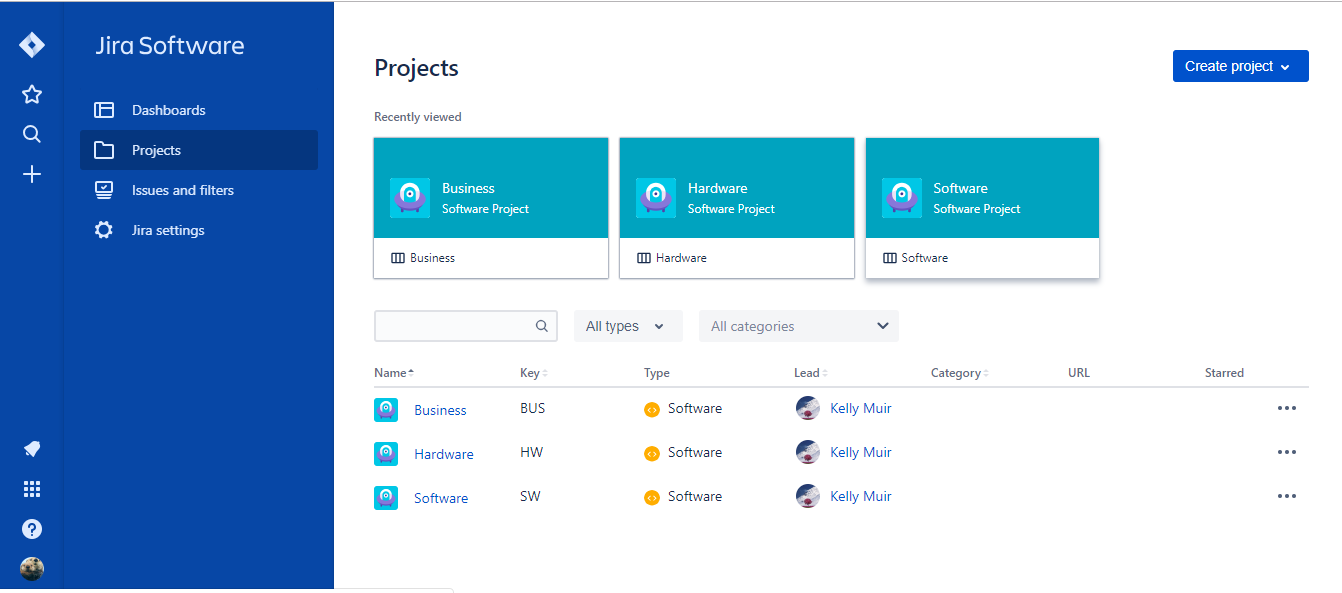
\includegraphics[width=.6\textwidth]{02_09-10/images/jiradash.png}
    \caption{Jira Dashboard}
    \label{fig:jiradash}
\end{figure}
\subsection{H1: Develop intake prototypes}

After the whole team watched the game video, several members began prototyping mechanisms to intake and sort cubes. Because the game requires the robot to pick up minerals that are inside the crater, the robot either needs to be able to climb over the crater to intake the minerals, or extend some sort of intake over the crater wall. 

Kelly decided to try developing an intake mechanism that would allow the robot to stay outside of the crater, and reach over the wall, which would allow the team to continue using a mecanum drivetrain, for its increased maneuverability. The first concept they thought of was to extend a rake in front of the robot, on linear slides, that would pull the minerals back to the robot and up the crater wall. The rake would have tines spaced a little bit under 2.75 in apart, so the silver minerals would be pulled back, but not the gold minerals. This would allow the robot to cycle back and fourth between the crater and the silver depot, to score minerals as fast as possible. When this prototype was tested, Kelly found that the gold minerals could still be pulled back, when a silver mineral would get stuck in the tines of the rake, so the rake concept would not work to sort out the minerals. 

The next concept Kelly tested was a spinning surgical-tubing intake, similar to ACME's Velocity Vortex robot. By spinning the two stages of the intake in opposite directions, the minerals would first be pulled into the robot, and then pushed against the rake, expelling the gold minerals and allowing the silver to pass into the robot. This design relied on the fact that if the intake was extended over the outer boarder of the crater, any minerals in it would be inside the crater, and thus not subject to the two mineral maximum. This worked well to pull in the minerals once they were brought to the top of the crater wall by the rake, but the transition between the two counter-rotating brushes caused the minerals to get stuck, or rejected prematurely. 

After watching videos of robots from Res-Q, the last FTC game to involve the same game elements, Kelly decided the surgical tubing intake was worth pursuing, because it could quickly bring minerals to the top of the robot one at a time, which would be necessary for sorting them out. Kelly built a new prototype that had the surgical tubing whips mounted directly over one another and rotating the same direction. Ashlin built a acrylic back plate and funnel that would guide the minerals up the intake, and allow only one to pass through the top at once. Kelly built a simple sorting system that consisted of two parallel bars mounted far enough apart to allow the gold to pass through, but not the silver. When this was combined with the spinning intake, the minerals would be sucked up into the robot, and then divided into gold and silver. 

After Jon finished the prototype for the intake he began to find the optimum distances the needed to be from the ground, crater edge, and edge of the robot. This is because these measurements are vital for CADing and fabrication. Jon found that the optimum distance from the robot to the roller was 7 inches. While the optimum distance from the floor to the roller was 4 inches. 
\begin{figure}
    \centering
    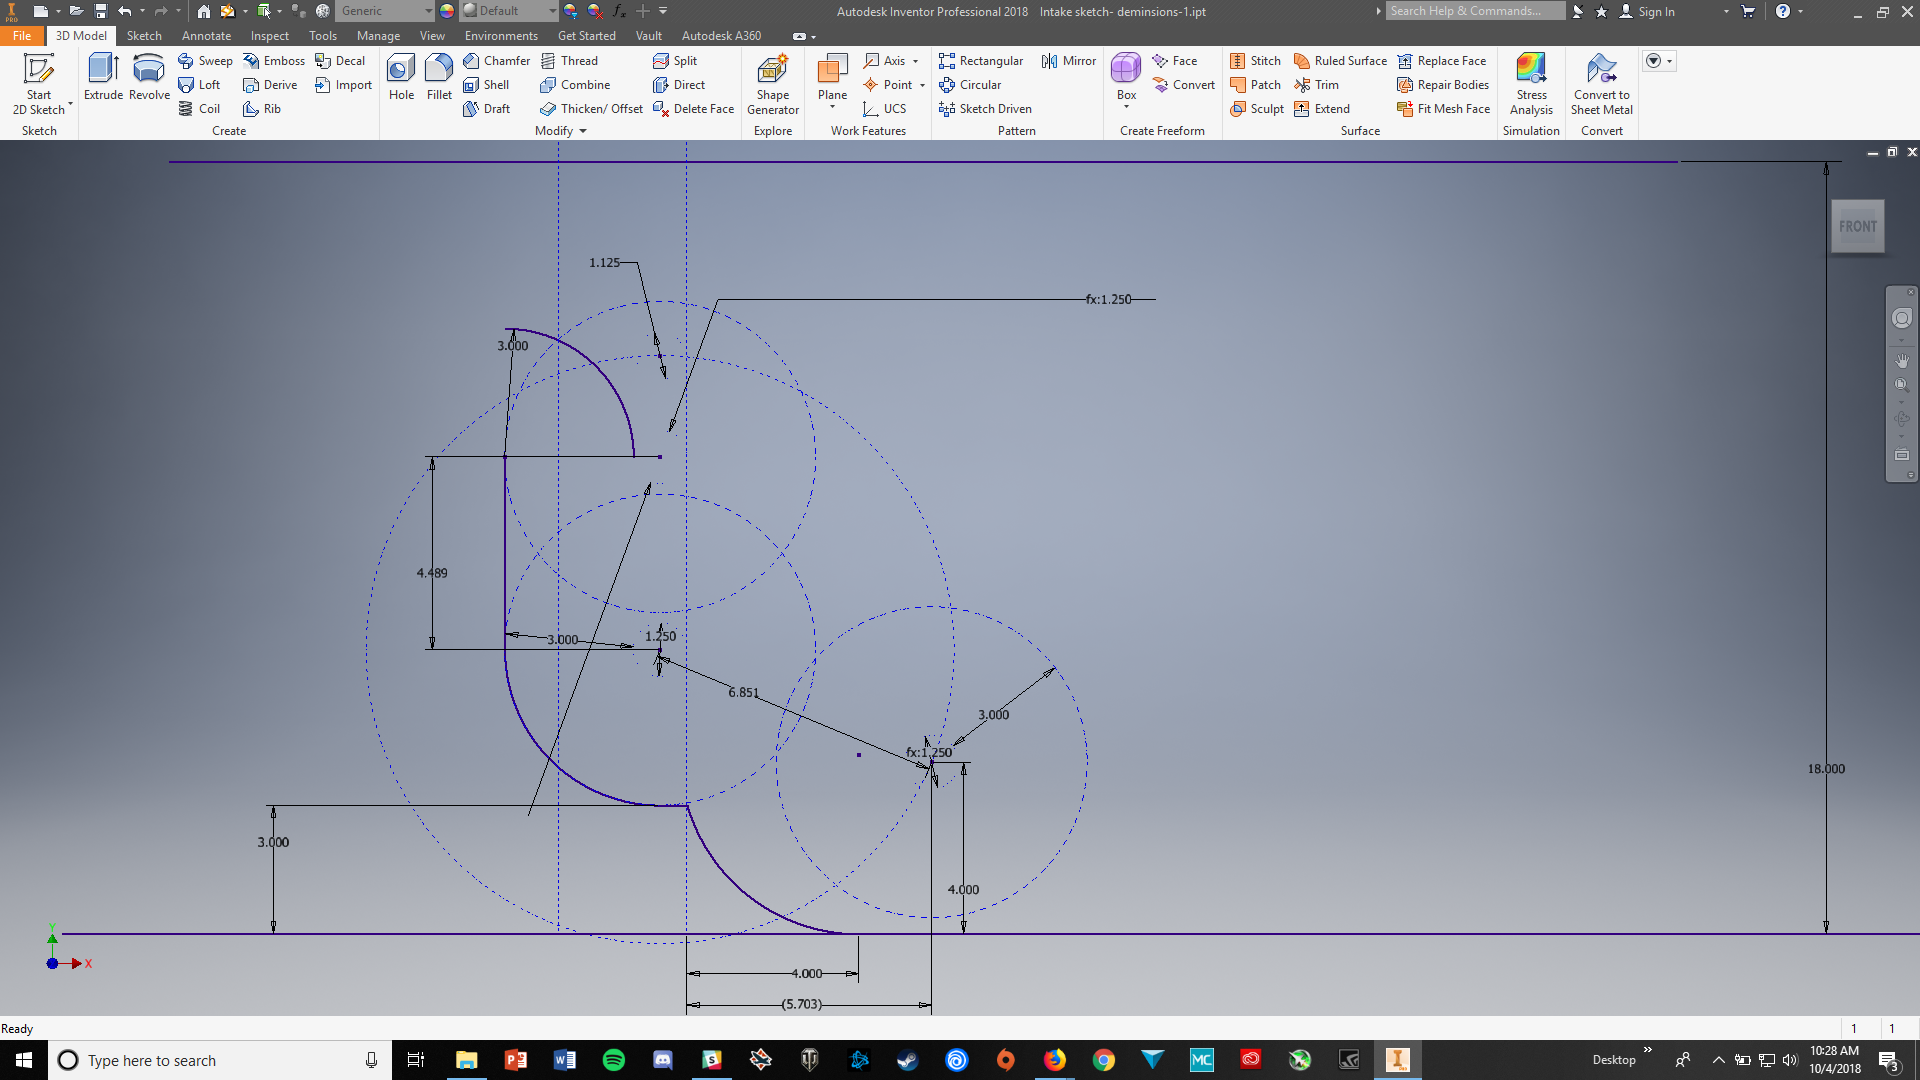
\includegraphics[width=.6\textwidth]{02_09-10/images/intakesketch.png}
    \caption{Deploy-able intake dimensions}
    \label{fig:intake}
\end{figure}



\subsection{H2: Investigate possible drivetrain designs}

Given that a good drivetrain is vital for a successful robot, the team needed a solid design. The team decided there were two ways of going about creating a good drivetrain for the Rover Ruckus challenge. The first was to design a drivetrain capable of going inside the crater. The team thought this might be a good idea seeing as the intake design would be simpler and we could traverse all areas of play. This would need to be a drivetrain with very good traction, torque, and durability. For this purpose the team looked into a drop-center tank design (WCD) or a tracked design. Suspension was also considered. These were considered because both WCD and tracked designs are very effective at traversing rough or bumpy terrain. Like the crater rim. Jon did research in this area and found a simple suspension (bell crank) design and sketched a few ideas for a tracked drive train (fig 0.1). After discussing these together, and WCD, the team decided that going into the crater was probably not necessary. Thus, the team stopped development on these ideas and continued pursing the second way of going about designing a drive train.



\begin{figure}
    \centering
    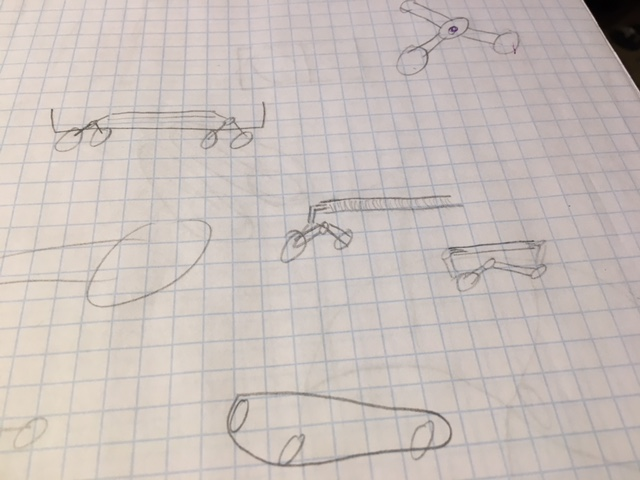
\includegraphics[width=.6\textwidth]{02_09-10/images/IMG_0256.JPG}
    \caption{Bell crank suspension and tracked drivetrain sketches}
    \label{fig:drivetrain sketches}
\end{figure}



\subsection{H3: Develop Drivetrain Prototypes}

Shawn and Ben worked on developing a rocker bogie drivetrain to test. The drivetrain used two different rotation points on both sides to be able to get over things, such as the crater wall. They used a picture from the Internet to assist in the construction of the drivetrain. After it was finished, the drivetrain worked as expected but wasn't quite within the size constraints. Sadly, the drivetrain had to be taken apart. 

\subsection{S1: Test vision software}

Finding the gold particle at the beginning of the autonomous posed many challenges for the software team. Modifying a python vision script from the Relic Recovery season, Emma and Kelly were able to successfully detect the gold particle. However, the problems started when they realized that with the robot starting above the ground, the camera would have full view of the crater full of gold particles behind the line of particles they were trying to detect, as seen in
Figure \ref{fig:camera}.

After discussing possible solutions, including identifying the three particles first (both silver and gold), Emma decided to experiment with camera angles from approximately five inches above the field. Without having the field nor the mounting point on the robot, Emma tried her best to find the optimal position for the camera, although a final position will need to be determined once the robot is complete. 

Although there are different ways to solve this problem using programming, for simplicity's sake, Emma is hoping to troubleshoot more with the camera when the field arrives sometime in the next week. As they already have functional code, it would be beneficial to only have to position the camera correctly. 

\begin{figure}
    \centering
    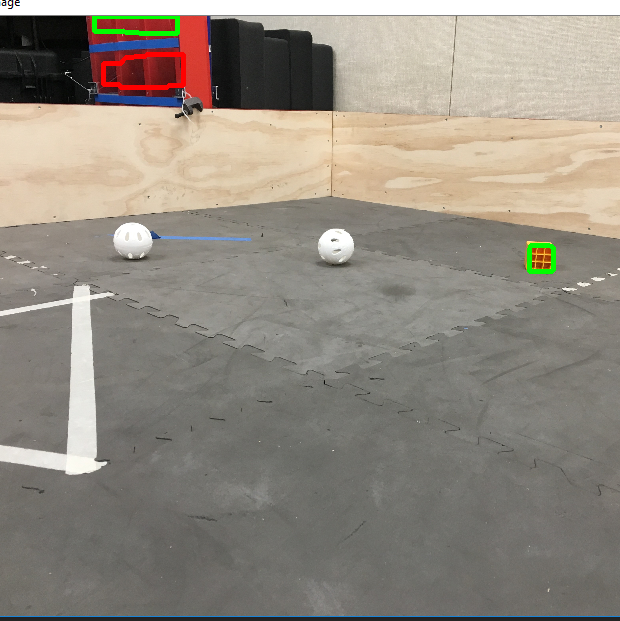
\includegraphics[width=.6\textwidth]{02_09-10/images/originalcameraposition.png}
    \caption{Original Position of the Camera}
    \label{fig:camera}
\end{figure}



\subsection{S2: Experiment with new motor controller features}

New motor functionality added with v4.0 of the SDK and the new Rev Expansion Hub firmware has the ability to have a PIDF control loop on the Rev Hub itself. This means that rather than commanding some vague `power' to the motor, and then having to empirically determine the relationship between this power and the velocity of the motor, you can directly command a velocity, and the control loop on board the hub will match that velocity regardless of voltage droop. After upgrading the firmware in the hubs and testing this functionality with a lone motor, Kelly re-wrote the MecanumDrive class to take advantage of it. After deploying this to the Relic Recovery robot, Kelly found that the robot was much easier to control. Without any feed-back control on the robot controller side, the robot was very stable, and it was much easier to move the robot slowly, because the hub would now do the work of closing a loop around the velocity of the robot.\clearpage \newpage \section{Week \thesection} 
\subsection{Hardware Goals}
\paragraph{H1: Work with intake prototypes}
 Test intake prototypes. 
\paragraph{H2: Develop a Team Marker}
 Design a team marker that will be used at the tournaments.
\newpage
\subsection{H1: Work with intake prototypes}

After looking further into the dual flywheel intake design, Jon and Kelly decided this was not a practical option because it would be difficult to fit onto the robot and create an efficient chain setup. Kelly and Jon then decided to go with a swing down roller design, as this would be easy to fit into the existing design and will likely work just as well. After deciding this, Jon built a prototype for this new intake. 

\begin{figure}
    \centering
    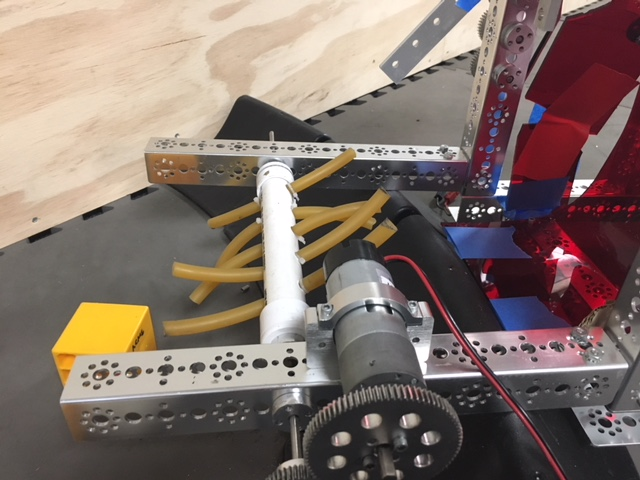
\includegraphics[width=.6\textwidth]{03_09-17/images/IMG_0262.JPG}
    \caption{Deploy-able intake prototype}
    \label{fig:my_label}
\end{figure}

\subsection{H2: Develop a Team Marker}

Shawn and Ben were tasked with developing a team marker. The team marker should fit within the size constraints and, ideally represent something about the team. Ben and Shawn decided to make a prototype anvil marker that could roll. Ben sketched out an anvil in his notebook and measured the height of cardboard. Based on this measurement, he divided the drawing into equal sections that were that height. Shawn the cut out the cardboard pieces and they pieced it together.\clearpage \newpage \section{Week \thesection} 
\subsection{Hardware Goals}
\paragraph{H1: Sorting Mechanism}
 Design a sorting mechanism to sort the minerals. 
\paragraph{H2: Investigate potential lift designs}
 Figure out which lift designs would work the best for the robot. 
\paragraph{H3: Design lift gearbox}
 Design a lift gearbox that can move the lift quickly and can lift up the robot. 
\subsection{Software Goals}
\paragraph{S1: Integrate the hub feedforward functionality into trajectory followers}
Integrate the new feedforward functionality into the trajectory code for auto paths.
\newpage
\subsection{H1: Sorting Mechanism}

Ashlin, Aidan and Kelly worked on the process for sorting the cubes from the balls. The first idea was a mechanical sorting system that would function like a coin sorter, allowing the cubes to fall through while the balls rolled past. This design was discarded because it took too much space and was not consistent. A new sorting system involved a color sensor and a U shaped cup. In figure \ref{fig:Sorter Version 2} the new system is shown connected to a prototype robot. The cube or ball would roll into the U-cup and then be read by the color sensor. The U-cup would then rotate about 135 degrees clockwise or counterclockwise to deposit the cube or ball in the corresponding cartridge. This idea did not work because there were not available servos that could rotate the required 270 and the system required too much space. This failed sorting system led to a third sorting system that was based around version two but took up less space and did not have to rotate as much. The final design, figure \ref{fig:Final Sorting Mechnism}, allowed the ball or cube to go into the rotating circle part where it would be read by the color sensor and then a servo would rotate the circle part about 45 degrees clockwise or counterclockwise to deposit it in the corresponding cartridge. This system worked significantly better because it allowed there to be only 90 degrees of rotation needed by the servo, the process would be significantly shorter, and the whole system could be condensed to take up no more than a 6 inches.

\begin{figure}
    \centering
    \includegraphics[width=.6\textwidth]{04_09-24/images/sorter.jpg}
    \caption{Sorter Version 2}
    \label{fig:Sorter Version 2}
\end{figure}

\begin{figure}
    \centering
    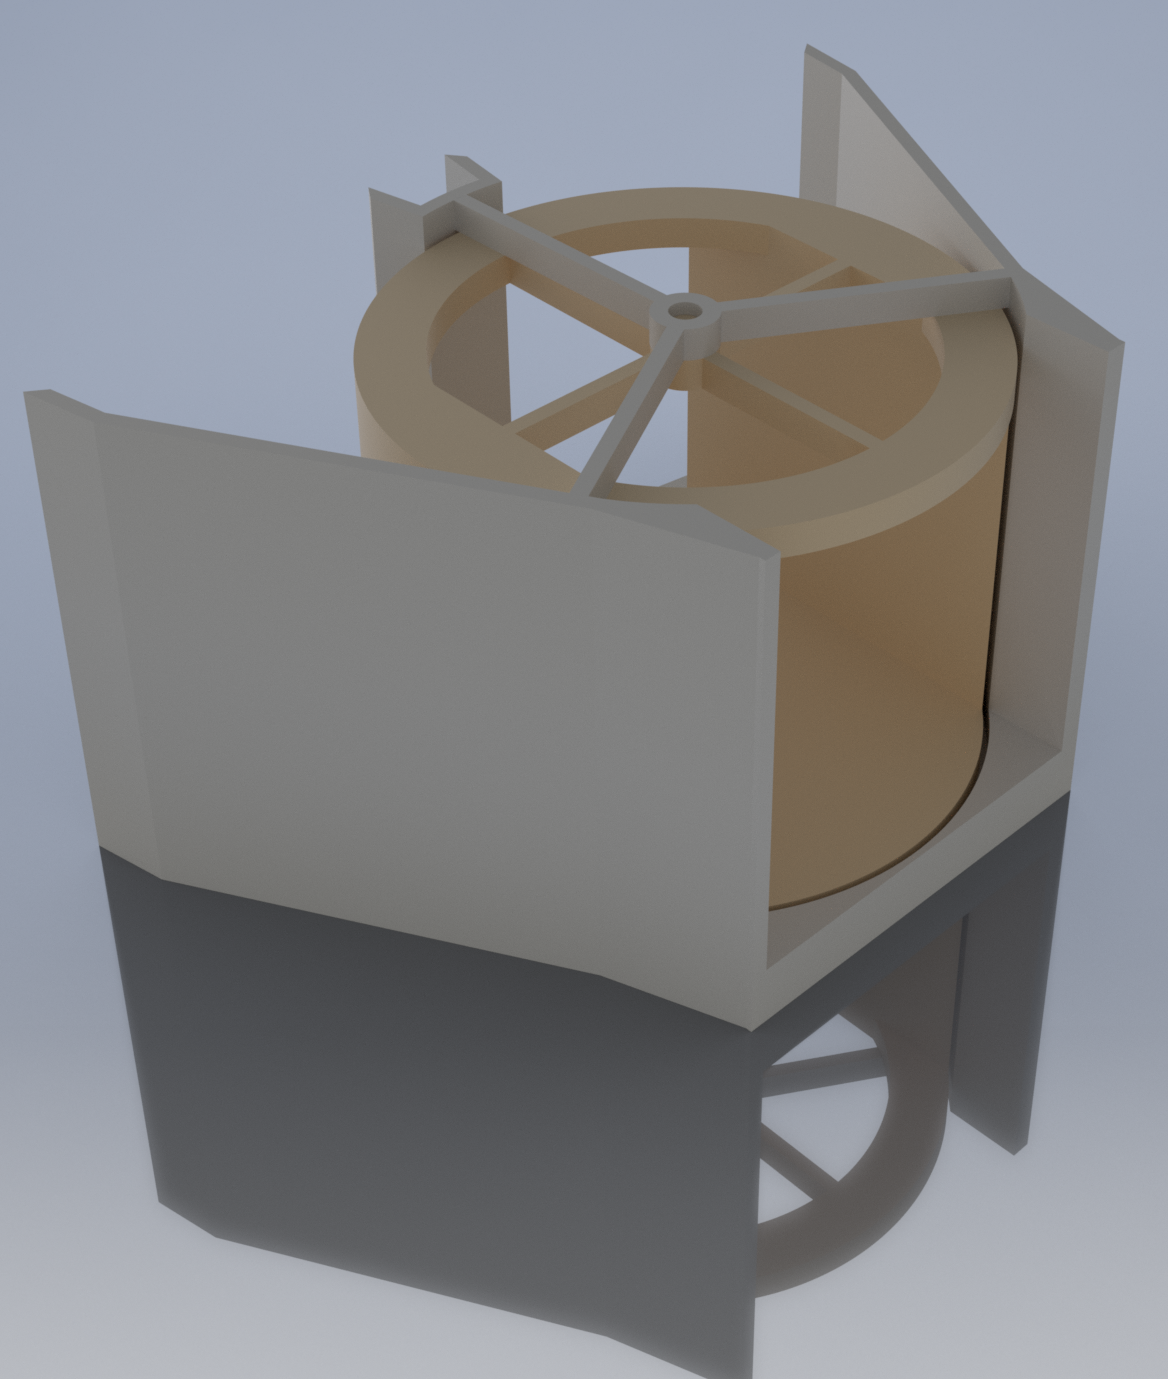
\includegraphics[width=.6\textwidth]{04_09-24/images/sorter2.png}
    \caption{Final Sorting Mechanism}
    \label{fig:Final Sorting Mechnism}
\end{figure}

\subsection{H2: Investigate potential lift designs}

The lift is going to be one of the most important mechanisms on the robot this year, as it is required for both scoring and latching. It will also need to be capable of moving very quickly, when carrying minerals to the top of the lander, and powerful enough to lift the entire robot off the ground at the end of the match. Because the team had only used Rev linear motion kits and drawer slides before, Kelly investigated the other options available for linear motion. Any potential solution needed to be capable of extending to the top of the lander, which is 32 inches off of the surface of the field, which would require two 16 inch stages, or three shorter stages. Because the lander bracket is only about four inches above the top of the robot, the mechanism that will attach to the lander only needs to be mounted to the first stage, meaning that any subsequent stages do not need to be as robust, as they will only ever bear the weight of the scoring system, not the robot itself. These requirements are quite similar to the FRC challenge last year, Power Up, which required teams to lift blocks above their robot to score, and then hang from a bar. Team 254, in particular, had a design that is super promising. It consisted of two fixed rails, a box-like first stage than ran between the fixed rails, and a smaller second stage carriage that ran within the first stage frame. Since this overall form factor fit all of the requirements, the team decided to settle on it for now, and investigate hardware that it could be constructed from. Team 254 constructed their lift out of square aluminum tubing and bearings that would roll against the surface, making it super fast and smooth. While this provides the best performance, the main drawback to this approach is the difficulty in manufacturing the brackets that mount the bearings to the tubing to the tolerances necessary to make everything run smoothly. If any parts are out of alignment or not parallel, then it gets a lot harder to move the lift. Another pre-fabricated option that many teams used last year to extend their relic arms over the field wall is Actobototics x-rail. The x-rail has a v-shaped groove on each side of its cross-section, allowing a v-bearing to run in the track. This would cut down on the number of bearings needed for the lift, because each pair of bearings can constrain the lift in two dimensions, not just one. If the bearings are aligned so that the majority of the forces go radially into the bearings, rather than axially, than it could be quite robust. Kelly configured the lift using these parts, and then put together a list of parts necessary to construct the lift. Because the brackets are pre-fabricated, the tolerances are much tighter than could be achieved if the team manufactured them. 
\begin{figure}
    \centering
    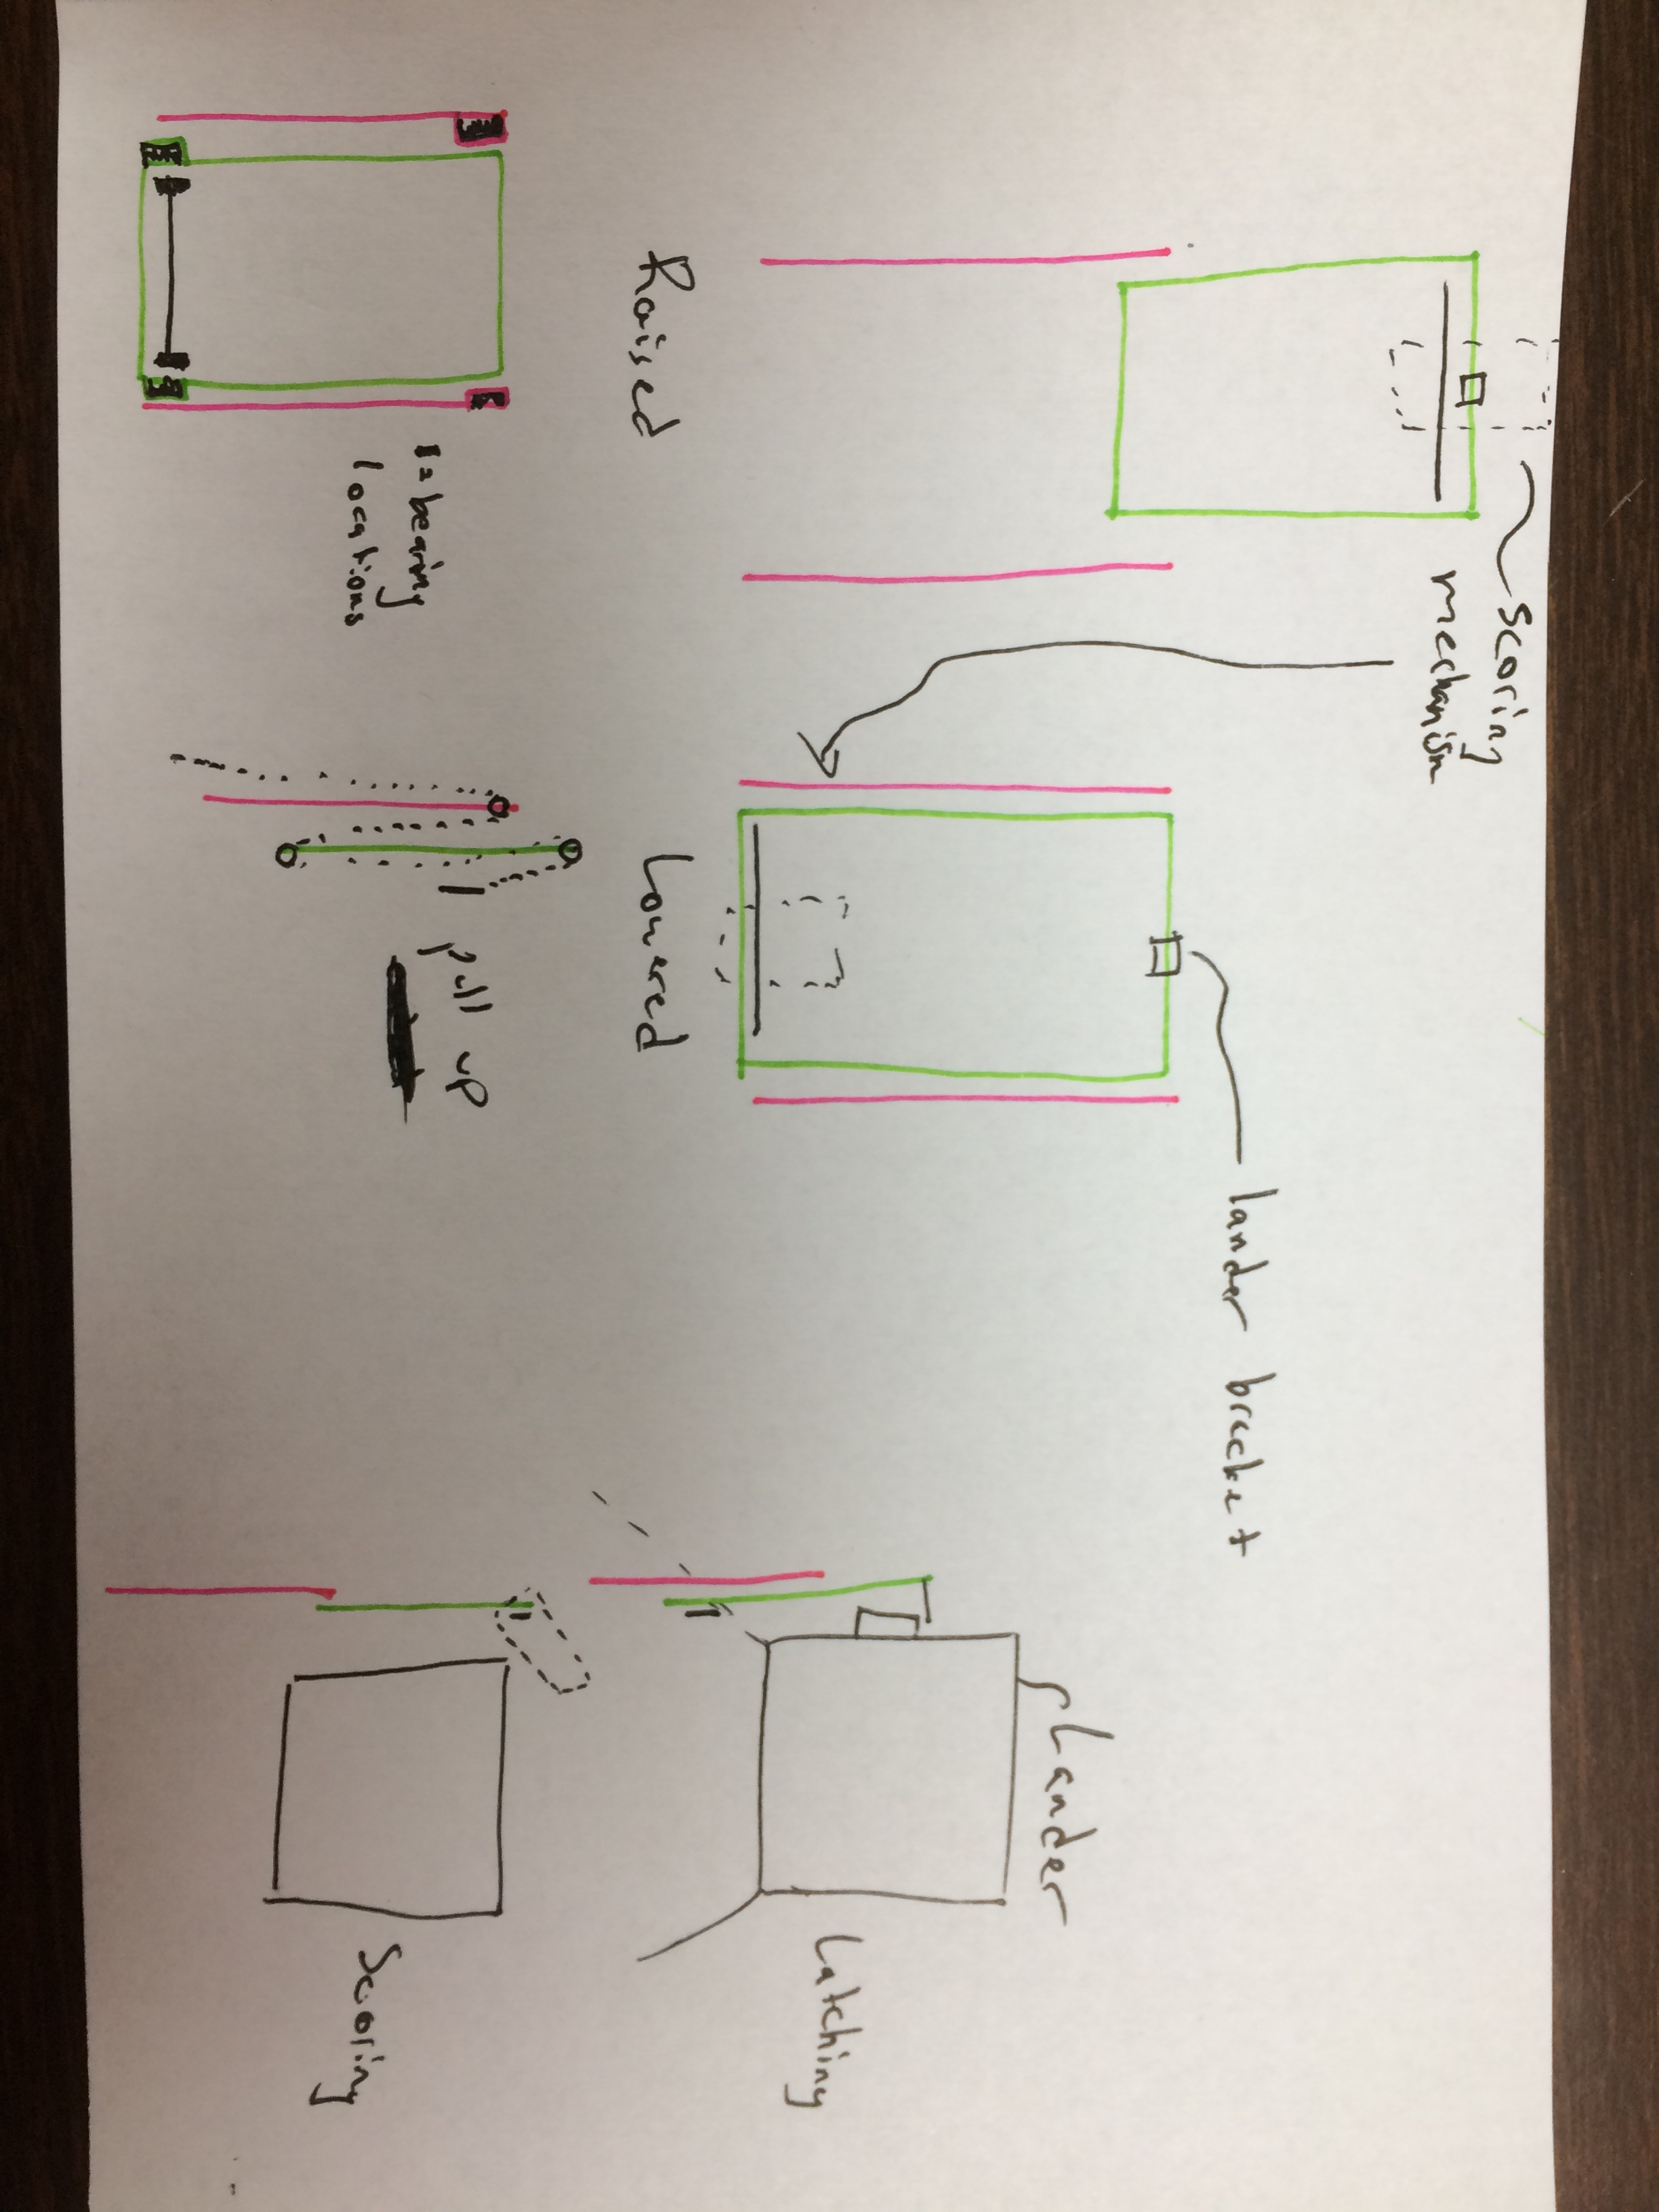
\includegraphics[width=.75\textwidth]{04_09-24/images/lift.jpg}
    \caption{Lift concept sketches}
    \label{fig:lift}
\end{figure}

\subsection{H3: Design lift gearbox}

Another goal for the lift was finding a suitable gearbox that would fit all of the requirements for the lift. During this process, Kelly decided against a shifting gearbox because of the necessary complexity, which meant that at least two motors would need to be used to get sufficient torque to lift the robot at the gearing necessary to make the lift fast enough. A ratchet would also need to be involved so that the robot could hang from the lander without powering the motors, making it easier to start and end the match. After researching options for a dual-motor gearbox, Kelly settled on a Versa Planetary from VexPro, because it could use a dual motor input to drive one gearbox from two motors, removing the need to join the two motors after the reduction and was modular meaning any custom gear ratio could be created; it could also be integrated with a ratchet kit to allow for one-way rotation when lifting off the ground. After assuming that the robot would weigh the full 20 kg, and requiring the motor to be able to accelerate it at 2g, a 25:1 reduction would be necessary. This should be enough to lift the scoring mechanism to the top of the robot in 1.5s, so the gearbox should be sufficient. Kelly added the necessary parts to the order sheet.

\begin{figure}
    \centering
    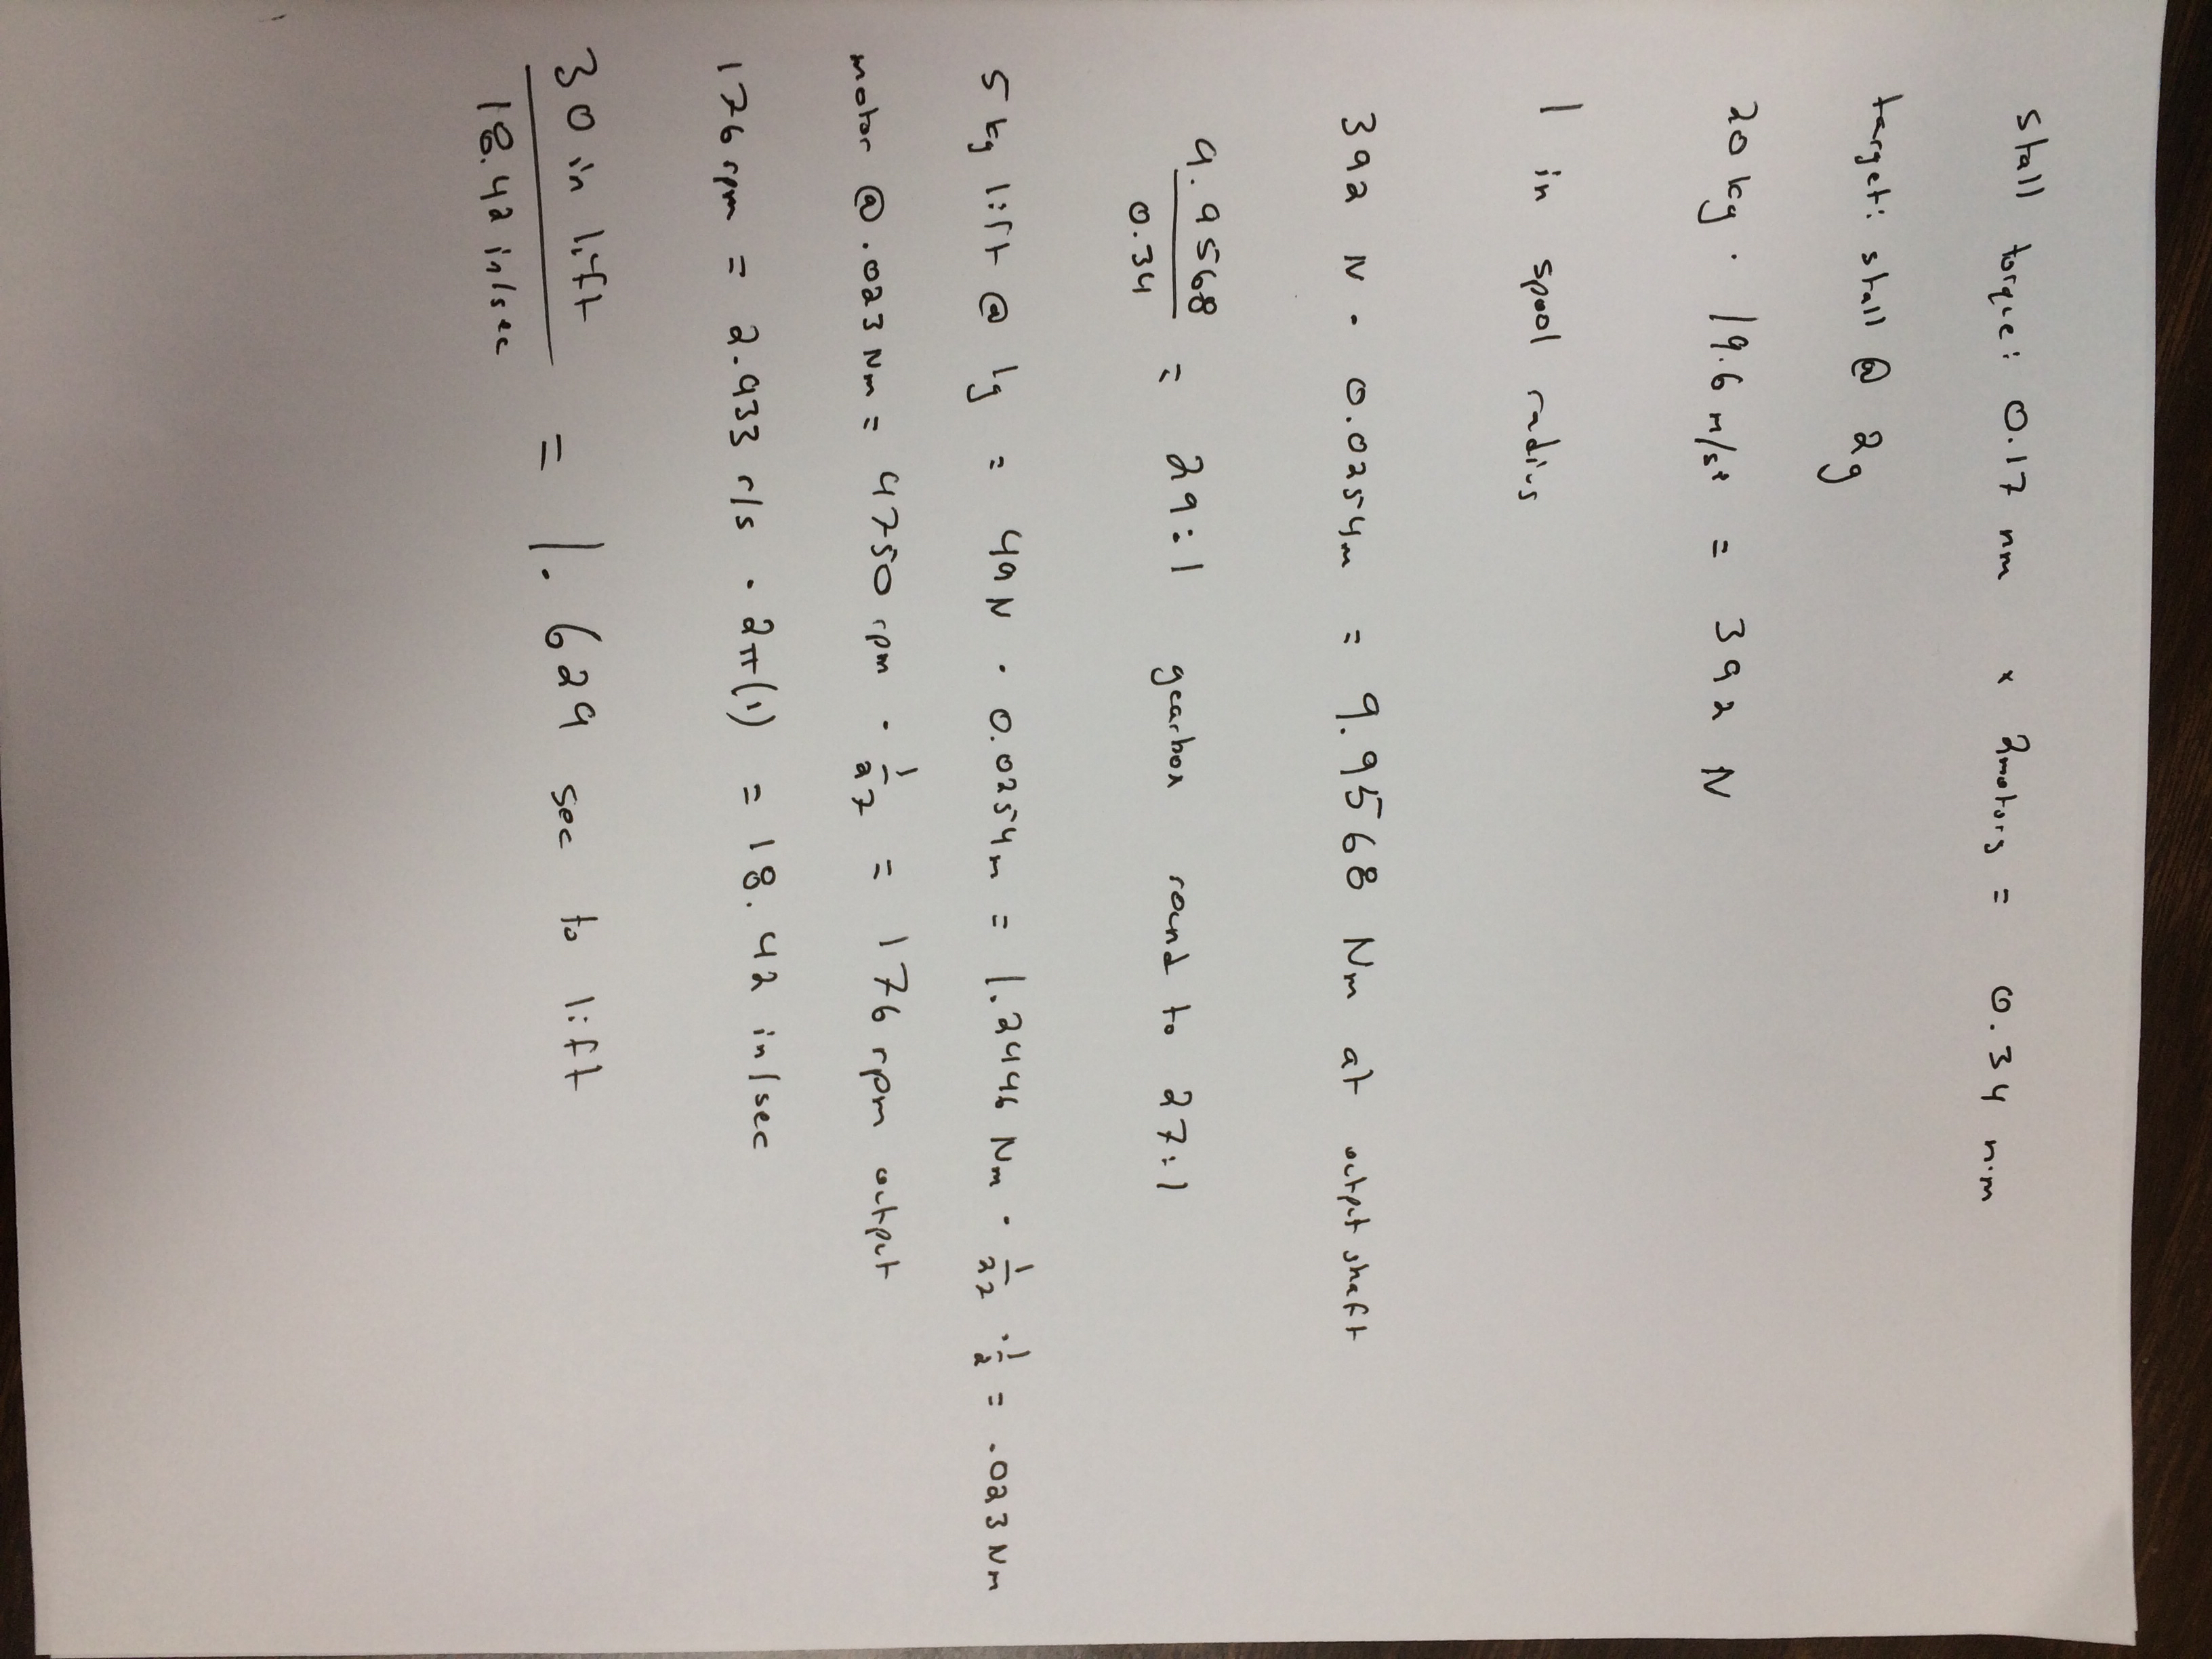
\includegraphics[width=\textwidth, angle=90]{04_09-24/images/math.jpg}
    \caption{Lift gearbox math}
    \label{fig:my_label}
\end{figure}
\subsection{S1: Integrate the hub feedforward functionality into trajectory followers}

Before, with each update of the control system, the trajectory would return a target velocity at that given moment, which would be multiplied by the empirically determined coefficient that would convert it to a power to command to the motor. The target position of the trajectory would be compared to the actual position of the robot, and a PID loop would use this error to correct the power commanded to account for the error. Now, the velocity returned by the trajectory is directly commanded to the motor, and the rev hub does the work of converting that to a voltage that is applied to the motor. The positional error still is accounted for, but now by correcting the commanded velocity, not the commanded power. Even with very low gains on the Positional PID loop, this yielded markedly better results than the previous trajectory follower, because of the new functionality in the Rev Hubs. The second necessary change to the trajectory follower was the way error was calculated. Previously, positional error was split into two components, axial and lateral, but the axial error was always parallel to the robot's heading, and the lateral error was always perpendicular to it. Because the new pathing system treated the drive completely holonomically, this no longer made sense, because when the robot was strafing, the axial error would be normal to its direction of travel, but when the robot was driving forward, the axial error would be tangent to its direction of travel. If the robot was moving through a curve with constant heading, always on the path but 1 inch behind where it wanted to be, the error would first be primarily axial, and then primarily lateral, which would cause strange behaviours when these errors are fed into separate PID loops. To counteract this, Kelly changed it so that the axial error was always tangent to the robot's direction of travel, and the lateral error was always normal to the robot's direction of travel. This improved the usefulness of the error measurements.

\begin{lstlisting}[language=Java]
public synchronized Pose2d update(double t, Pose2d pose, TelemetryPacket packet) {
        if (t >= duration) complete = true;
        
        Pose2d targetPose = path.get(axialProfile.get(t).getX());
        double theta = path.deriv(axialProfile.get(t).getX()).pos().angle();
        Pose2d targetVelocity = path.deriv(axialProfile.get(t).getX()).times(axialProfile.get(t).getV());

        Vector2d trackingError = pose.pos().minus(targetPose.pos()).rotated(-theta);
        Vector2d trackingCorrection = new Vector2d(
                axialController.update(trackingError.getX()),
                lateralController.update(trackingError.getY())
        );

        double headingError = pose.getHeading() - targetPose.getHeading();
        double headingCorrection = headingController.update(headingError);

        Pose2d correction = new Pose2d(trackingCorrection, headingCorrection);
        return targetVelocity.plus(correction);
    }
\end{lstlisting}
\clearpage \newpage \section{Week \thesection} 
\subsection{Business Goals}
\paragraph{B1: Discuss Gracious Professionalism}
 Discuss the important FIRST value of Gracious Professionalism with both teams.
\subsection{Hardware Goals}
\paragraph{H1: Continue Developing The Team Marker}
 Creating a releasing mechanism for the team marker. 
\paragraph{H2: Drivetrain decision}
 Decide on the design for the drivetrain.
\paragraph{H3: Develop X-rail based lift}
 Develop a CAD model of the x-rail based lift.
\subsection{Software Goals}
\paragraph{S1: Start Working on Lift Kinematics}
 Begin to work on lift kinematics for the robot.
\newpage
\subsection{B1: Discuss Gracious Professionalism}

Although ACME members from last year were well versed in the ways of Gracious Professionalism, the new members - and ARES members - were not. As Gracious Professionalism is the underlining value of FIRST, Emma and Kelly decided to give a presentation on the subject. Pulling up a Google Slides presentation in the Drive, Emma was able to write a fairly comprehensive guide on how to be a Gracious Professional. After having Kelly read it over, and spending some time developing the Flowers Dialectic, Kelly presented it to both teams. The teams had a great discussion about how and how not to behave at competition, as well as how to be a Gracious Professional in their everyday life. The only thing this presentation could not totally explain was how rewarding it can be to practice these values. The team especially saw this last year at the Northern California Regionals, when they helped their friends, team 5214: Tech Support, by buying them an emergency servo. The team ended up being on the winning alliance because of it.  
\subsection{H1: Continue Developing The Team Marker}

Shawn and Ben hadn't quite finished the anvil when they realized that the marker had no deployment mechanism and it looked super bad. They then decided to go with just a cube with a loop that could be dropped by a servo over the side. Shawn was tasked with making the block and he made it out of acrylic. Then Ben used basic Tetrix to make a servo mechanism that would unhook the cube and make it fall. Ben built the mechanism and found that a lot of servos didn't work.

\begin{figure}
    \centering
    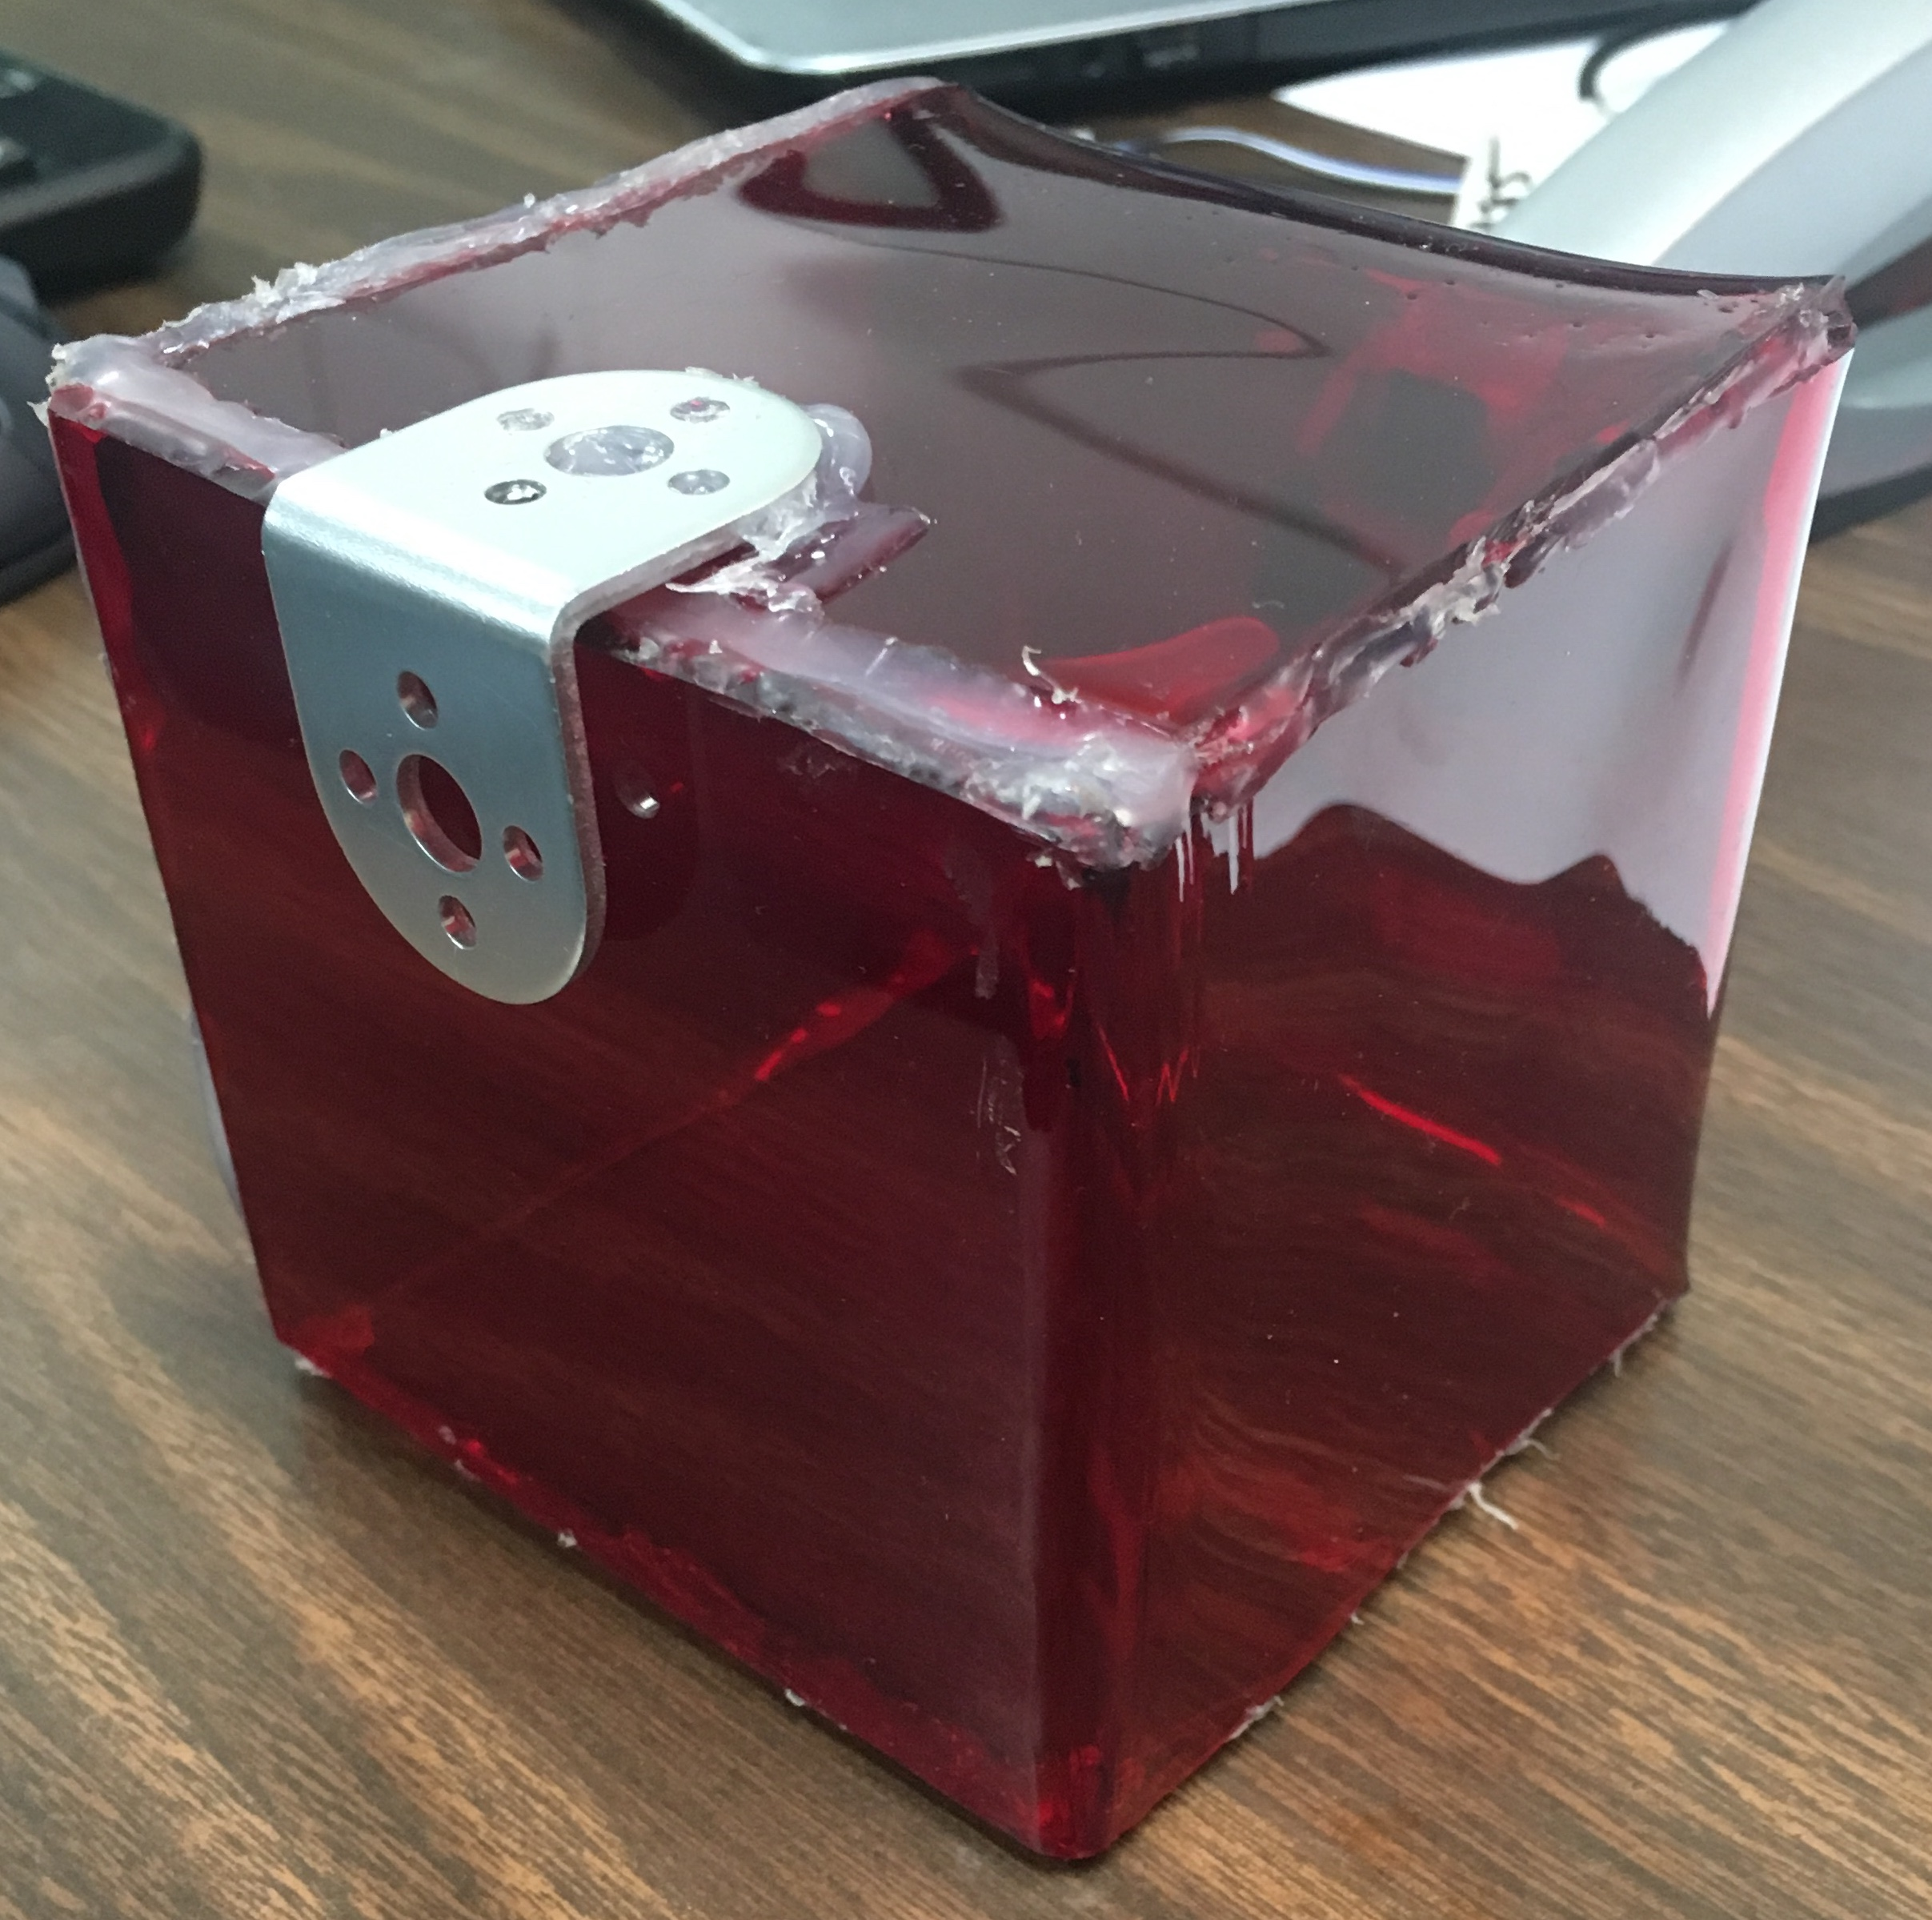
\includegraphics[width=.6\textwidth]{05_10-01/images/cube.jpg}
    \caption{Acrylic Cube}
    \label{fig:cube}
\end{figure}



\subsection{H2: Drivetrain decision}

The entire team made a matrix to help weight the pro and cons of the prototype drive-trains and already proven styles. The matrix took a lot in to consideration, such as agility, size, strength, traction, and maneuverability. The results of the matrix was a mecanum style drive-train driven by orbital 20 gearbox and belts. We choose this style because of its high speed, agility, and maneuverability, the downside to this style drive-train is the traction, which in turn can make playing defense a lot hard, compared to a none mecanum drive-train.  


\subsection{H3: Develop X-rail based lift}

 After downloading all the required parts from Actobotics website and importing them into Inventor. He began assembling them per the design previously created. The first issue that had to be resolved was the mounting of the bearing bracket onto the x-rail. Because the maximum amount of space should be left on the inside of the lift, a mounting scheme other than the one suggested by Actobotics would have to be used. By swapping out the standoffs that came with the kit for shorter ones, the bearings could be brought closer to the x-rail they were attached to, reducing the spacing between stages to about a quarter inch. This reduced clearance between the stages necessitated another change. The default mounting hardware would fit, but as soon as bolts were added to the model the bolts would collide with the opposite rail. To resolve this, separate mounting hardware had to be found on the Actobotics website, allowing the bolts to clear each other. It would still be necessary to use lower profile 6-32 bolts than the standard Tetrix ones, but they should be able to be found at a hardware store. The inner carriage turned out to a be a little different than planned. There was no way to run more bearings along the front and back of the first stage box, because those grooves were already occupied by the bearings fixed to the top of the fixed stage. This meant that for the second stage to mount, a second piece of x-rail would have to be attached to the inside of the first piece, allowing the carriage to attach to it, or the carriage would have to run along the inside of the first stage. This would be possible with x-rail, because if the bearings pressed against the inside, the v-groves would prevent it from rotating forward and back, provided the top and bottom sets of bearings were spaced far enough apart to reduce the force applied laterally. This, however, would necessitate a different mounting strategy, because the brackets would have to attach to the end of the x-rail, rather than the sides. Unfortunately, the hole pattern on the end of the x-rail did not nicely match up with the hole pattern on the bracket, so Kelly decided to put two smaller vertical pieces of x-rail on either side of the cross-brace that would support the scoring mechanism, and then mount the bearings to that. 
 
 \begin{figure}
     \centering
     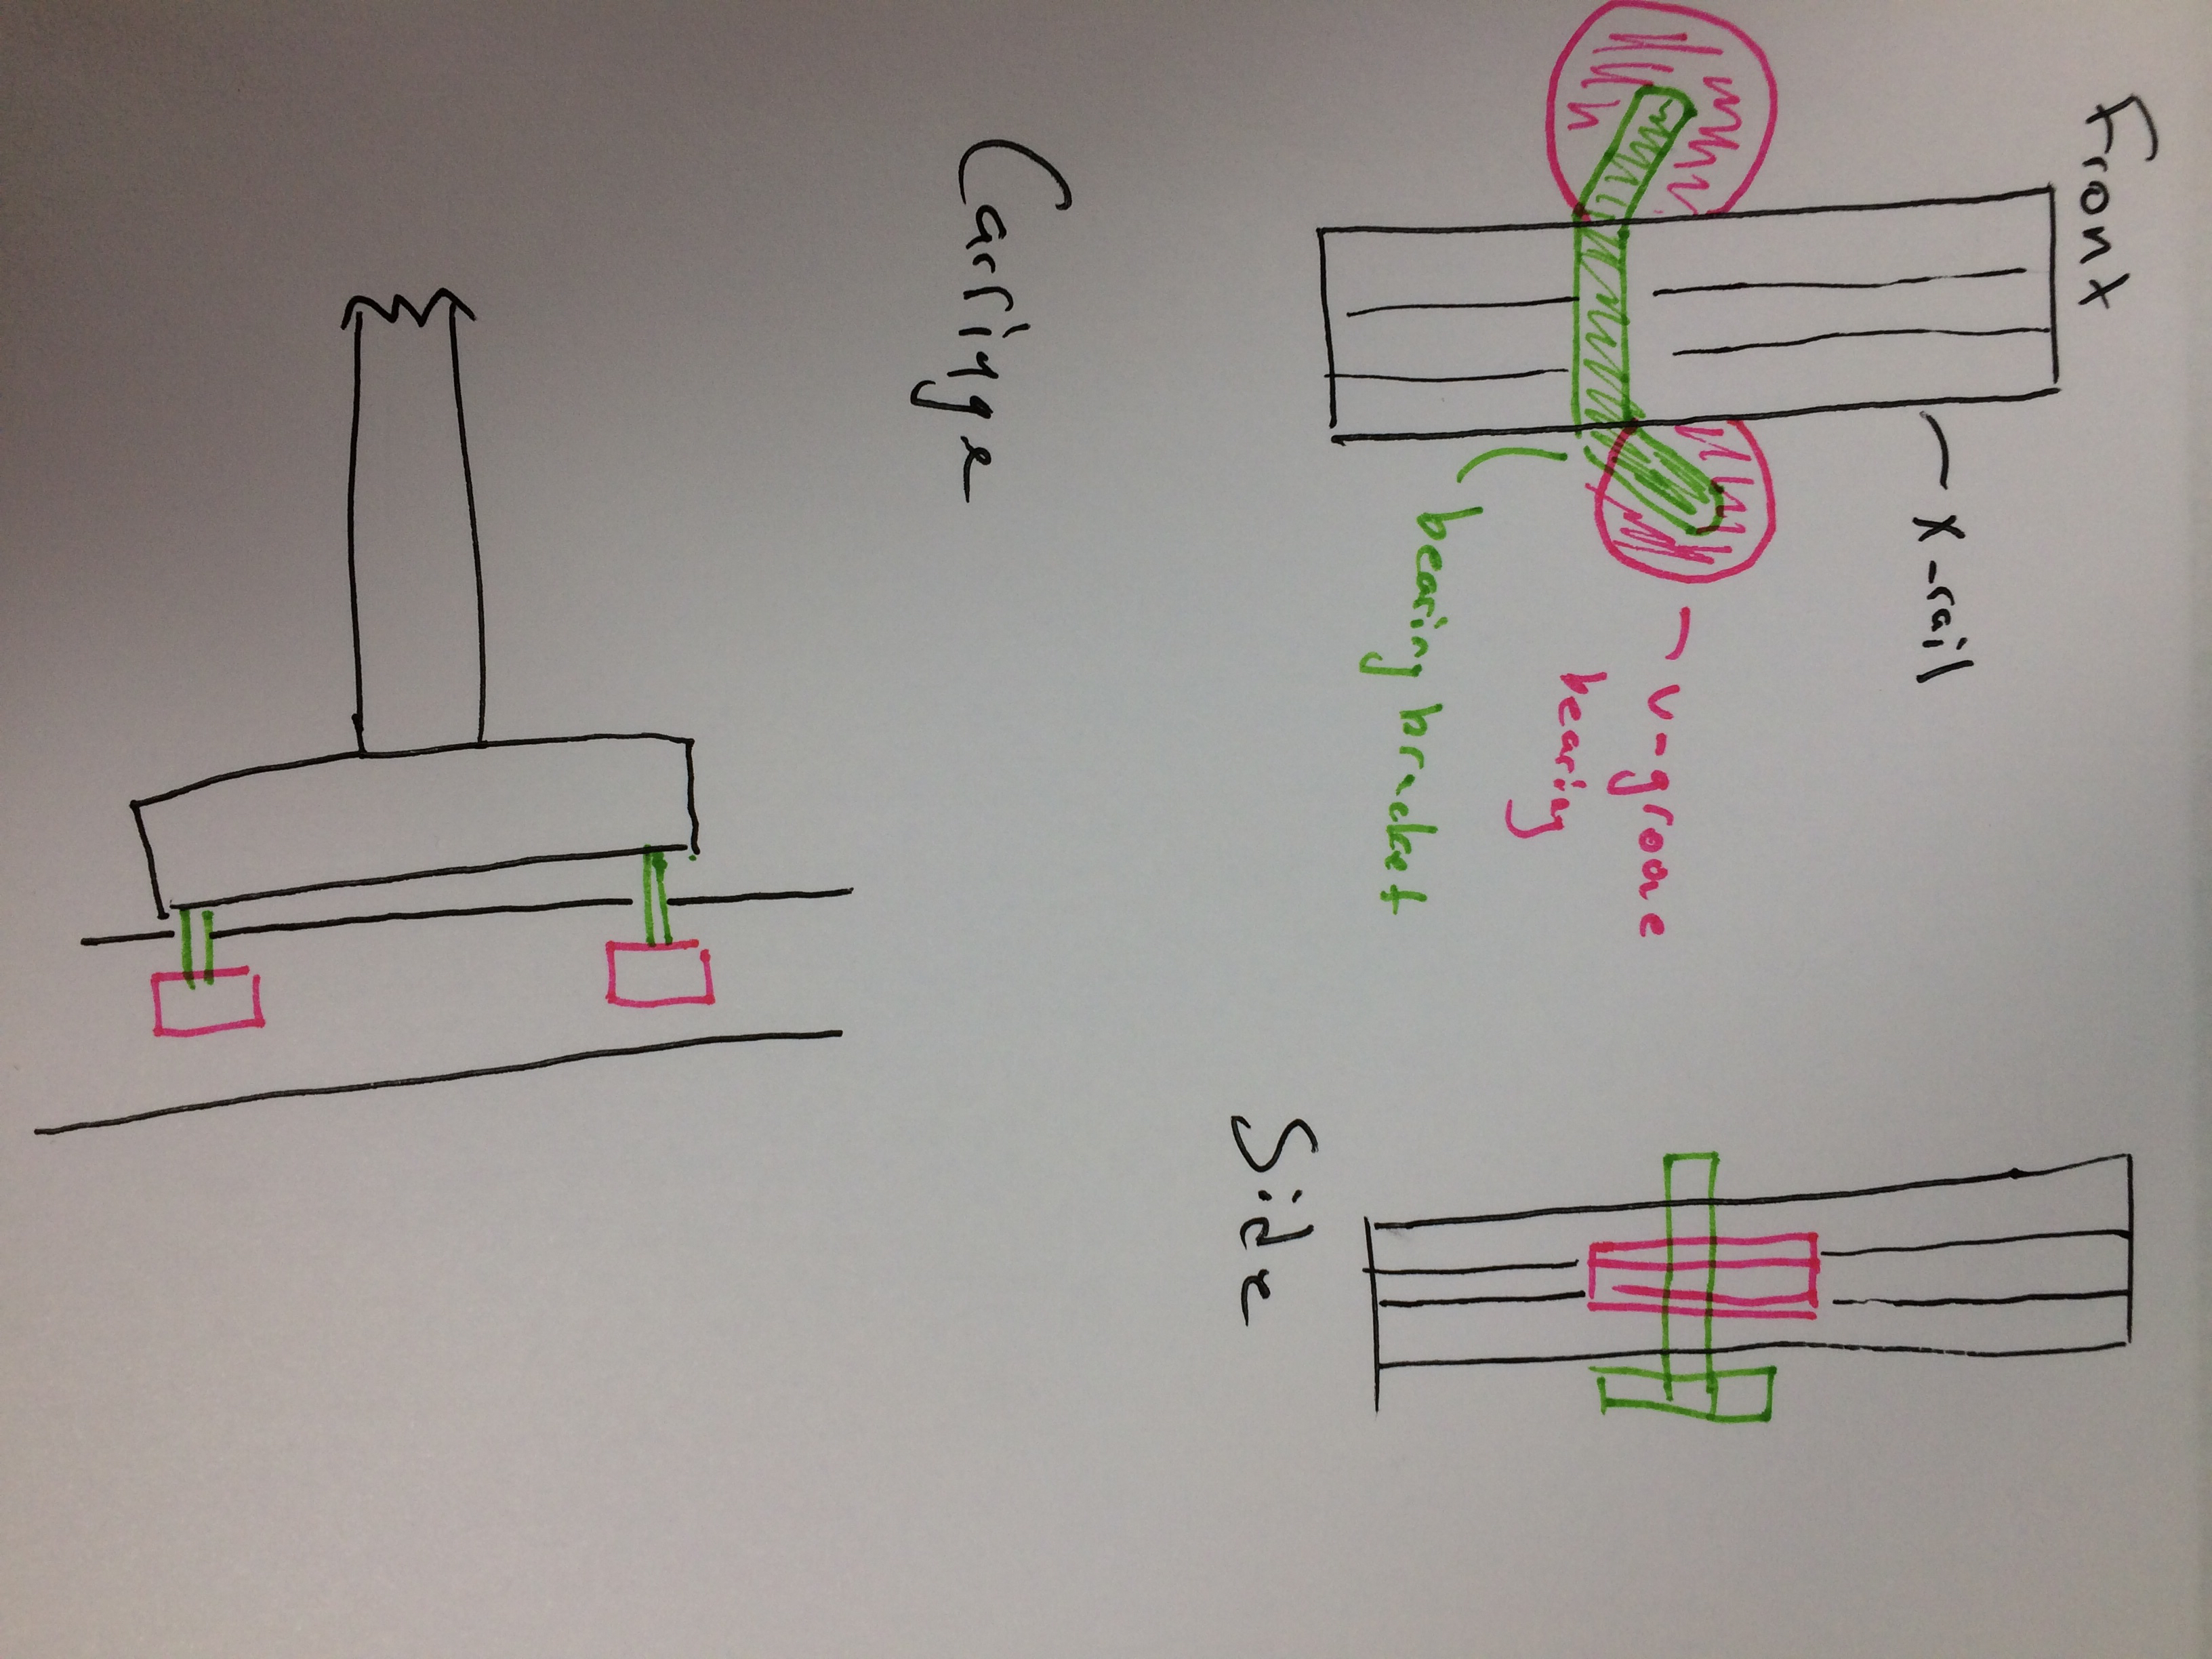
\includegraphics[width=.6\textwidth]{05_10-01/images/xrail.jpg}
     \caption{X-rail detail view}
     \label{fig:my_label}
 \end{figure}
\subsection{S1: Start Working on Lift Kinematics}

This week, Emma began to work on lift code for the robot. There were several things that the team needed the lift to do. First there needed to be a driver controlled portion of the code so that drivers could manually lift and lower the lift. The other modes needed were run to position; where the lift could go to a certain position and hold position; so that the lift will stay at the position it is currently at. Emma used an enum for this. Enums are excellent for storing data that doesn't present as textual or numerical data, which is why they are ideal for this situation. Emma also learned how we use motion profiling on the robot. It is important to integrate motion profiling into the lift so that movements are as smooth and precise as possible. Here is the code that Emma wrote this week.
\begin{lstlisting}[language=Java]
    private enum LiftMode{
        DRIVER_CONTROLLED,
        HOLD_POSITION,
        RUN_TO_POSITION;

    }
            switch (liftMode){

    public void goToPosition(double position){
        liftProfile = MotionProfileGenerator.generateSimpleMotionProfile(
                new MotionState(0, 0, 0, 0),
                new MotionState(position, 0, 0, 0),
                1, 1, 1 //find real values eventually
        );
        liftMode = LiftMode.RUN_TO_POSITION;
        startTime = System.currentTimeMillis();

    }
\end{lstlisting}
A motion profile is generated every time goToPosition is called. Emma is hoping to work on the other modes next week.
\clearpage \newpage \section{Week \thesection} 
\subsection{Hardware Goals}
\paragraph{H1: Sorter CAD}
 CAD the sorter.
\paragraph{H2: Develop custom lift}
 Further investigate possible lift designs and weigh the pros and cons of each. 
\paragraph{H3: CAD Lander Clamp}
 Create a latch in CAD that will be used to attach to the lander. 
\paragraph{H4: Finalize robot design}
 Discuss the final robot design with the team.
\subsection{Software Goals}
\paragraph{S1: Continue working on lift kinematics}
 Continue developing software for the lift.
\newpage
\subsection{H1: Sorter CAD}

Ashlin and Aidan continued to finalize the sorting system for the robot and completed the CAD model of the sorter. Aidan realized a flaw with the system, if a ball then a cube went into the sorter right after each other then the cube could jam the sorter. This was because the interior length of the rotating piece was almost 4 inches long, so if a ball then a cube went in the sensor would read the ball and then start rotate but the cube would block the rotating and jam the servo. Kelly, Ashlin, Aidan, and Jon all thought of ideas to solve this problem including shortening the sorter's dimensions, creating a servo powered gate, or just changing the whole system. The team finally decided to solve the problem once the sorter was fabricated. The problem could only occur if the two items went into the sorter immediately after each other. The team believed that the intake would probably space out the items sufficiently so this problem wouldn't occur, and if it did occur small adjustments could be made to increase the space between items.

\subsection{H2: Develop custom lift}

The x-rail lift design would work, but Kelly still wanted to investigate the 254-style lift, with square tubing, bearings, and custom bearing blocks. While more labor-intensive and harder to pull off, the end result would be better than with x-rail if it turned out correctly. Where the x-rail only needed bearings on one side, because the v-bearings would be able to resolve both radial and lateral loads, normal bearings can only resolve radial loads, so bearings will have to be placed on at least three sides to constrain the lift in both dimensions. Since the lift is composed of two mirrored parts, connected by the frame of the first stage, Kelly could get away with only running bearings along three sides of each tube, excluding the outer one, because the bearings in the y-axis would push the two sides against each other, preventing the lift from shifting side-to-side. Each bearing assembly would consist of four bearings, two on either side of the tube pinching it, and two next to each other running along the inside of the tube. Kelly began the CAD by making 1 in by $\frac{1}{2}$ in by $\frac{1}{16}$ in wall aluminum tubing in 16 inch lengths. One of these would be mounted to the drivetrain, and the other would make up the vertical portion of the first stage, rolling along the fixed one. A bearing assembly would go at the top of the fixed one and the bottom of the moving one, keeping the bearings as far apart from each other as possible, distributing the load and stabilizing the lift. The inner carriage would be made out of a H-shaped arrangement of more tubes, with a bearing assembly mounted at the top and bottom of each side of the H. After considering mounting the bearings by sandwiching the tube between two machined plates, Kelly realized this would not support the inner bearings, so decided on machined blocks that would be fixed to the tube with rivets. The blocks would have a quarter inch hole on the side for attaching the pinching bearings, and hole at the top where a bolt would connect the two blocks and support the inner bearings. After assembling this, Kelly found there was not enough room on the vertical portion of the first stage for both sets of bearings to roll against it, so it was neccecary for them to be swapped out for one inch by one inch tubes instead. 

\subsection{H3: CAD Lander Clamp}

To lower and raise the robot from the lander, the team decided to attach a latch to their lift. The team decided to do this because by attaching it to the scoring lift the team would not have to create a separate lift or arm to hang from. Kelly made the original prototype for this mechanism - which used two pillow blocks that when placed around the hook on the lander had a bar slid through to have the robot hang. Jon then used this basic prototype to CAD a more finalized design.

\begin{figure}
    \centering
    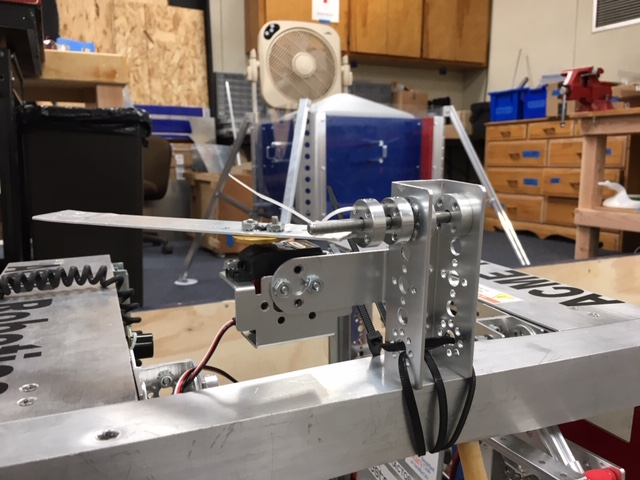
\includegraphics[width=.6 \textwidth]{06_10-08/images/latch1.JPG}
    \caption{Latch Prototype}
    \label{fig: Latch CAD1}
\end{figure}

\begin{figure}
    \centering
    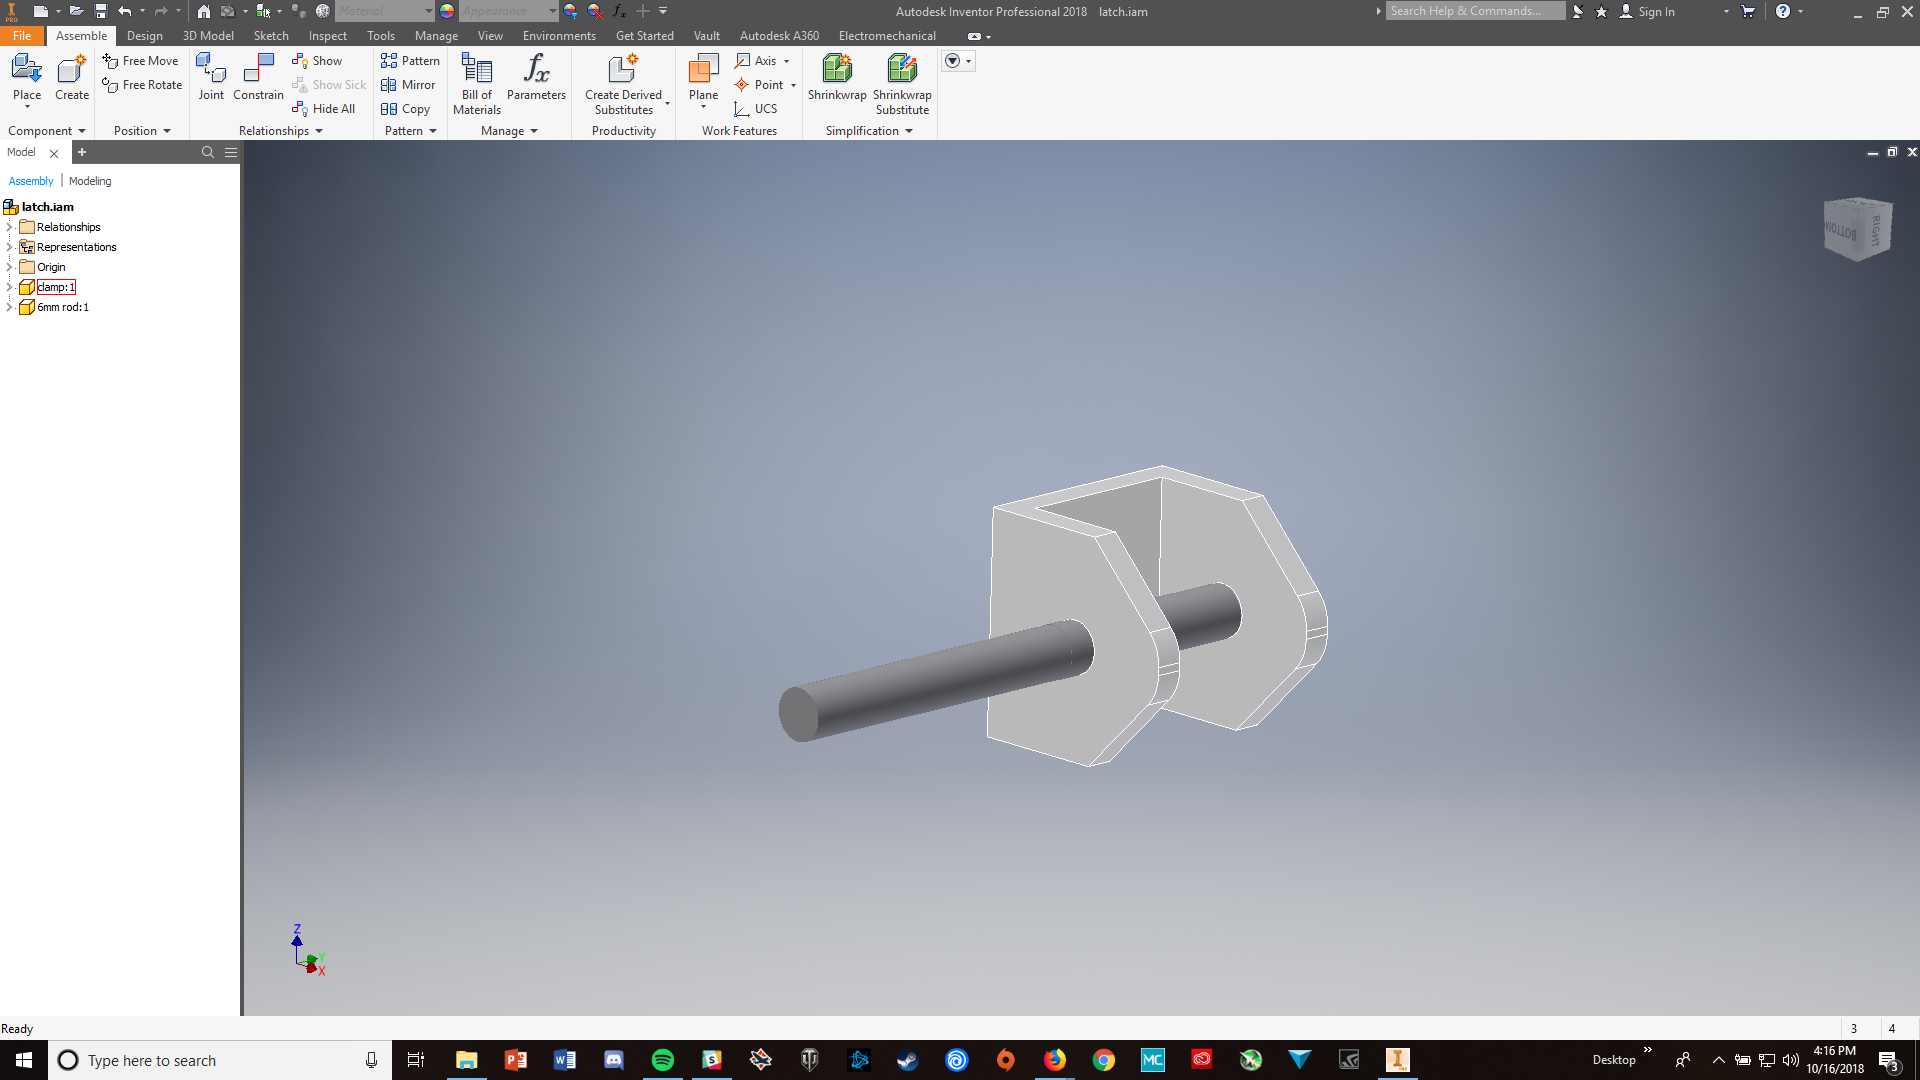
\includegraphics[width=.6 \textwidth]{06_10-08/images/latch.png}
    \caption{Latch CAD}
    \label{fig: Latch CAD2}
\end{figure}

\subsection{H4: Finalize robot design}

The team got together and went over the robot design, making sure that everything had been considered and accounted for before the final stages of CAD were completed and parts were ordered. Everybody presented prototypes and CAD that they had been working on, and the team decided whether or not to stick with it, and discussed any problems that might arise as the parts went into production. The first thing to decide was the type of drive base. The team had used mecanum drives the previous two years, and was confident they could build it correctly, but did not want to dismiss a tank drive. The tank drive that was being considered was a chain driven 6-wheel drop center west coast drive. The mecanum drive being considered was the same thing that the team had used to success last year, a belt-driven mecanum drive, with dead axles constrained between drive plates giving it extra rigidity. Oren had made some improvements over last year's design, including using smaller belts and swapping out parts to increase maintainability. The team decided they should use mecanum drive for its increased maneuverability unless a definite need for tank drive was needed. Because the defensive advantage given by the advantage of tank was countered by the maneuverability of mecanum and the ability to get out of tight situations, and the settled upon intake had no need for the robot to be able to go inside the crater, the team decided to go with a mecanum drive. The team decided to stick with the intake design consisting of a rake that would extend over the crater wall and pull minerals toward the robot and a series of surgical-tubing whips to suck the minerals in from there. The active sorter using a color sensor was chosen because it would be more reliable when the robot was in motion, and the double cartridge design was chosen because it would allow the two mineral types to be scored independently. Finally, the team decided to use the custom lift rather than the x-rail based one because Oren was confident that he would have the time to manufacture it to the neccecary specifications, and Dan felt it was something that would be able to be made on the manual mill at GSS.
\subsection{S1: Continue working on lift kinematics}

This week Emma continued to work on software for the lift. She wrote the code for the other modes that the lift needs to execute. These being the "hold position" and "driver controlled" modes. As stated in her last entry, Emma used a enum to switch between modes. Emma also experimented with motor encoders for the first time. Especially how you can use encoder ticks to find out how far up or down the lift has moved. Below is the code that she wrote. 
\begin{lstlisting}[language=Java] 
    private enum LiftMode{
        DRIVER_CONTROLLED,
        HOLD_POSITION,
        RUN_TO_POSITION;
    }

    private int inchesToTicks(double inches) {
        double ticksPerRev = liftMotor1.getMotorType().getTicksPerRev();
        double circumference = 2 * Math.PI * RADIUS;
        return (int) Math.round(inches * ticksPerRev / circumference);
    }

    private double ticksToInches(int ticks) {
        double ticksPerRev = liftMotor1.getMotorType().getTicksPerRev();
        double revs = ticks / ticksPerRev;
        return 2 * Math.PI * RADIUS * revs;
    }

    private double getLiftHeight(){
        return ticksToInches(getEncoderPosition());
    }

    private void setLiftHeight(double height){
        setEncoderPosition(inchesToTicks(height));
    }
    public void update(){

        double liftPower;
        switch (liftMode){
            case DRIVER_CONTROLLED:
                double start = getStartingPosition();
                double max = getMaxLiftPosition();
                double min = getMinLiftPosition();
                int currentPos = getEncoderPosition();
                setStartingPosition(start);
                setMaxLiftPosition(max);
                setMinLiftPosition(min);
                setEncoderPosition(currentPos);

                if(currentPos > start){
                    liftPower = this.liftPower;

                }else if(currentPos == start){
                    liftPower = this.liftPower;

                } else {
                    liftMode = LiftMode.HOLD_POSITION;
                };
                update();
                break;

            case HOLD_POSITION:
                double liftHeight = getLiftHeight();
                double error = pidController.getError(liftHeight);
                liftPower = pidController.update(error);

                break;

            case RUN_TO_POSITION:
                MotionState currrentState = liftProfile.get(System.currentTimeMillis() - startTime);
                break;
        }
    }
    public void goToPosition(double position){
        liftProfile = MotionProfileGenerator.generateSimpleMotionProfile(
                new MotionState(0, 0, 0, 0),
                new MotionState(position, 0, 0, 0),
                1, 1, 1 //find real values eventually
        );
        liftMode = LiftMode.RUN_TO_POSITION;
        startTime = System.currentTimeMillis();

    }
}
\end{lstlisting}
Of course there is more, as far as the variables and setters and getters, but this should give you the general idea. Through this Emma also realized that relying on getting the motor position to account for where the lift is at all times probably isn't very reliable. So she plans to use a Hall Effect sensor on the lift to narrow the field of possible positions.
\clearpage \newpage \section{Week \thesection} 
\subsection{Business Goals}
\paragraph{B1: Decide what business tasks need to be completed before the Burlingame competition}
 Create tasks in Jira that need to be executed before ACME's first competition.
\paragraph{B2: Finalize the budget with the team captains}
 Decide on the final budget for the build.
\paragraph{B3: Print, sign, address, stamp and send the fundraising letters}
 Completely finish the process of sending out fundraising letters to sponsors.
\paragraph{B4: Start interviewing team members for bios}
 Interview ACME members for their bios in the business notebook.
\subsection{Hardware Goals}
\paragraph{H1: Finish Designing the team marker}
 CAD the team marker.
\paragraph{H2: Complete Sorter and Intake CAD}
 Editing the Sorter and attachments.
\paragraph{H3: Testing Rev Linear Slide Kit}
 Build the linear slide system. 
\paragraph{H4: CNC Milled Drive-Train }
 Cut Drive-Train Plates.
\newpage
\subsection{B1: Decide what business tasks need to be completed before the Burlingame competition}

With the team's first competition confirmed, Emma thought it might be good to start figuring out what business tasks needed to be completed before hand. Using the business Jira board, Emma wrote up tasks that covered all areas of the business team. Such as, finishing fundraising letters, writing up the goals and action plan in the EN, and writing up ACME's outreach events in the EN. Having a list of tasks written out, whether on paper or on a screen, is better way to keep track of tasks rather than just having a running list in your head. Most of the tasks she created were specific to the EN and need to be completed before their first tournament. She will be working on several of these tasks in the weeks to come.

\subsection{B2: Finalize the budget with the team captains}

Finalizing the budget for the season was important to complete sooner rather than later because so many other tasks (especially business tasks) depended on it. Using the list of parts needed for the robot, the team was able to estimate how much all of the parts would cost (\$2500), including how many extras they were going to need to build spare parts just in case something broke on the robot. The team also left enough room in the budget to allow for iteration, if need be (\$700). That total came out to be \$2,200. As an extra precaution, the team decided to add about 30\% of wiggle room onto that total, bringing the total number to \$6000. The team thinks that this is a very reasonable number and is planning to reach it by sending out fundraising letters to the community. As the team is not supported by any school, it is important to decide the budget as early as possible in order to send them out quickly.

\subsection{B3: Print, sign, address, stamp and send the fundraising letters}

Although the fundraising letters were already written, the team still needed to print them out, address them, and mail them. Emma printed out over 50 individually addressed letters. Then, she, Kelly, and Sean and Eli from ARES signed their names at the bottom of the letters. ACME believes that this looks professional and adds a bit of a personal touch to each letter.  Eli and Sean addressed each envelope and the mentors sent them out later that day, as you can see in figure \ref{fig:Letters}. Both teams are expecting funds to come in the coming weeks. 

\begin{figure}
    \centering
    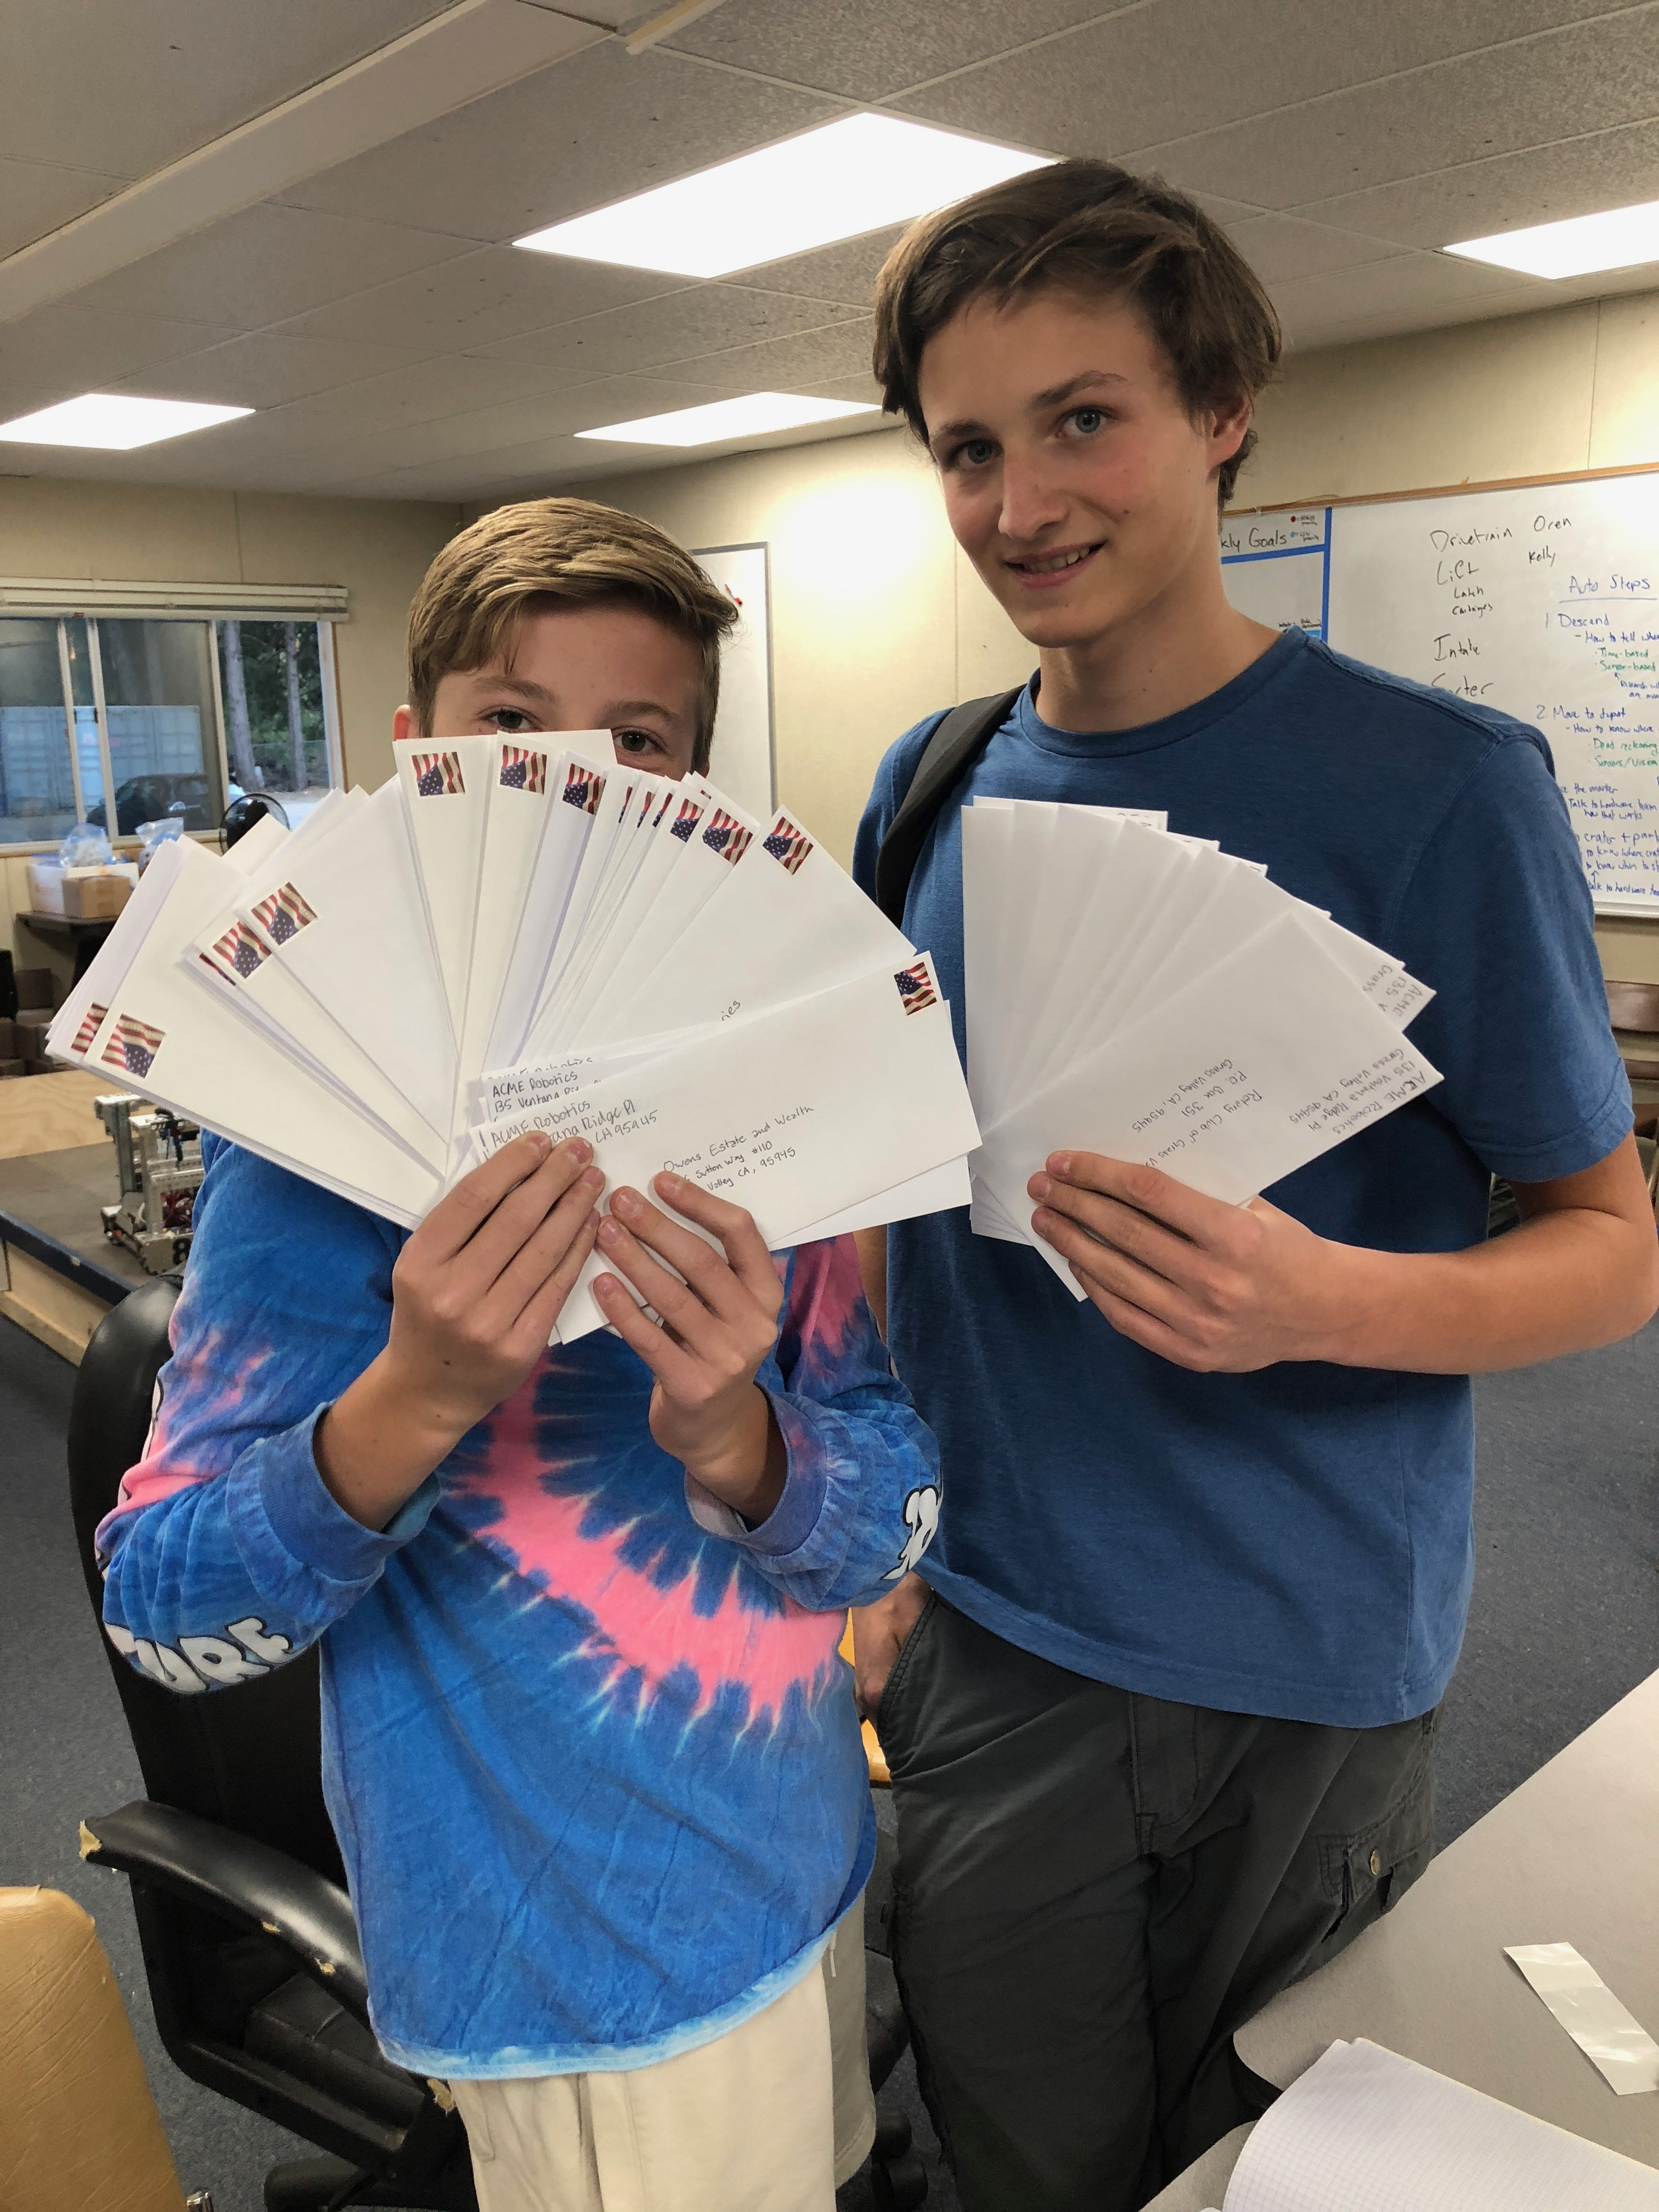
\includegraphics[width=.6 \textwidth]{07_10-15/images/letters.jpg}
    \caption{Eli and Sean with the final letters}
    \label{fig:Letters}
\end{figure}

\subsection{B4: Start interviewing team members for bios}

As always, the most distracting task of the season has come again. This is of course, interviewing members for their bios in the Business Notebook. Why is it so distracting to people? Because listening to Emma and Kelly give an interview to each member is for some reason very entertaining. Besides that they were able to gather all of the information that they needed. Some of the questions asked were, "What is your wildest idea for a FTC challenge?" and "What is your favorite gracious professionalism story?" Emma plans to type these bios up in \LaTeX along with a photo of each team member, as shirts and jackets arrive. 

\subsection{H1: Finish Designing the team marker}

Shawn and Ben worked on developing a new team marker that was an anvil. Ben took the old anvil hat CAD from last year and derived the file and re-scaled it to fit in the proper dimensions. Ben then added a hook and for the mechanism and engraved the top of the anvil with the team marker. They then rendered the model. At the next meeting, they further developed the mechanism.

\subsection{H2: Complete Sorter and Intake CAD}

Ashlin and Aidan worked on finalizing the attachment of the sorter to the intake and the rest of the robot as shown in \ref{fig:Intake CAD}. They put the sorter at a 45 degree angle to so that the objects would naturally go into the sorter and out into the cartridges easily because of the steep angle. Because of this they needed to edit the size of the cartridges so that the cartridges would have enough room to be raised up. They also attached a servo to the bottom of the sorter that it would be what rotates the sorter in either direction depending on if the item is a ball or cube.

\begin{figure}
    \centering
    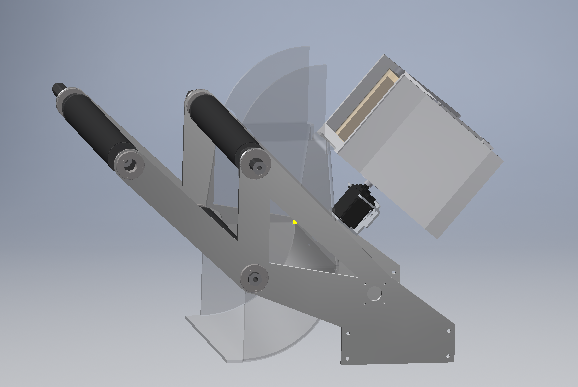
\includegraphics[width=.6 \textwidth]{07_10-15/images/IntakeCAD.png}
    \caption{Sorter and Intake CAD}
    \label{fig:Intake CAD}
\end{figure}

\subsection{H3: Testing Rev Linear Slide Kit}

Recently, the team received the Rev linear motion kits they ordered. To see how exactly the kit went together and see it would be mounted on the robot; Jon put some of the kit together. Jon made several segments, measured, and calculated the exact amount of 15 mm extrusion would be needed for the robot. This gave the team a better idea of how it would be assembled on the robot and a basis for CAD.

\subsection{H4: CNC Milled Drive-Train }

Oren, Ashlin, and Kelly worked with the Nu wood-shop teacher, to use their new CNC Laguna to cut out the 1/8 inch aluminum plates that make up the entirety of the drive-train. They had learn how to do auto tool changes and setting the X,Y and Z axis on the new tool as to allow them the most accurate product in the end\clearpage \newpage \section{Week \thesection} 
\subsection{Business Goals}
\paragraph{B1: Work on the Business Notebook}
 There is much to be done for the BN, so work on it must start immediately.
\subsection{Hardware Goals}
\paragraph{H1: Design of The Deployment Mechanism}
 Making marker deployer.
\paragraph{H2: Turn wheel inserts for the drivetrain}
 Fabricate the wheel inserts.
\newpage
\subsection{B1: Work on the Business Notebook}

The team realized that there was a lot of work that needed to be done on the Business Notebook, so Emma decided to take on that task. The BN includes all of the team's outreach events, the sustainability plan, our goals and action plans, team bios, fundraising information, current sponsor list, etc. With so much to, Emma decided to start with the team bios as those just needed to be typed in \LaTeX . Although there were plenty of answers to questions she and Kelly had asked team members the week before, she only chose 4 or 5 for each bio so that they only filled one page and would leave room for a picture. After the bios were completed, Emma started to write up the outreach events ACME did at the end of last season and over the summer. ACME had been writing about four paragraphs about each outreach event, which Emma thought was a bit excessive. So, she came up with a new format. A picture from the event is at the top of the page followed by the title for the event. A short summary sentence is after that, then bullet points highlighting parts of the event that explain what the team did, how it effected the team and how it benefited the people who the team helped or presented to. She found this method to be much more concise and easy to read. Next week, Emma plans to continue work on the BN by finalizing the budget and writing up the teams goals and action plans. \subsection{H1: Design of The Deployment Mechanism}

Shawn and Ben worked on revising and iterating the marker deployment mechanism. They discussed the best way to easily drop the marker and came up with a bar and hook mechanism.This mechanism works by setting a hook on a bar and then rotating the bar so the hook slides of the end and into the depot.

\subsection{H2: Turn wheel inserts for the drivetrain}

On Monday, Oren and Jon went to Datum Precision Machining to manufacture four wheel inserts which had been previously CADed. The team used Datum because they had a lathe that they were willing to let ACME use. Oren and Jon were not familiar with using a lathe so the owner of Datum, Jon, showed them the basics of operating a lathe. This was important because not only did critical parts for the robot made, but ACME created better ties with Datum and picked up useful skills. Now the team can hopefully continue to work with Datum when it needs parts manufactured. Oren and Jon knowing the basics of turning adds another tool in ACME’s belt as well as bolstering Oren’s and Jon’s individual know how.

\begin{figure}
    \centering
    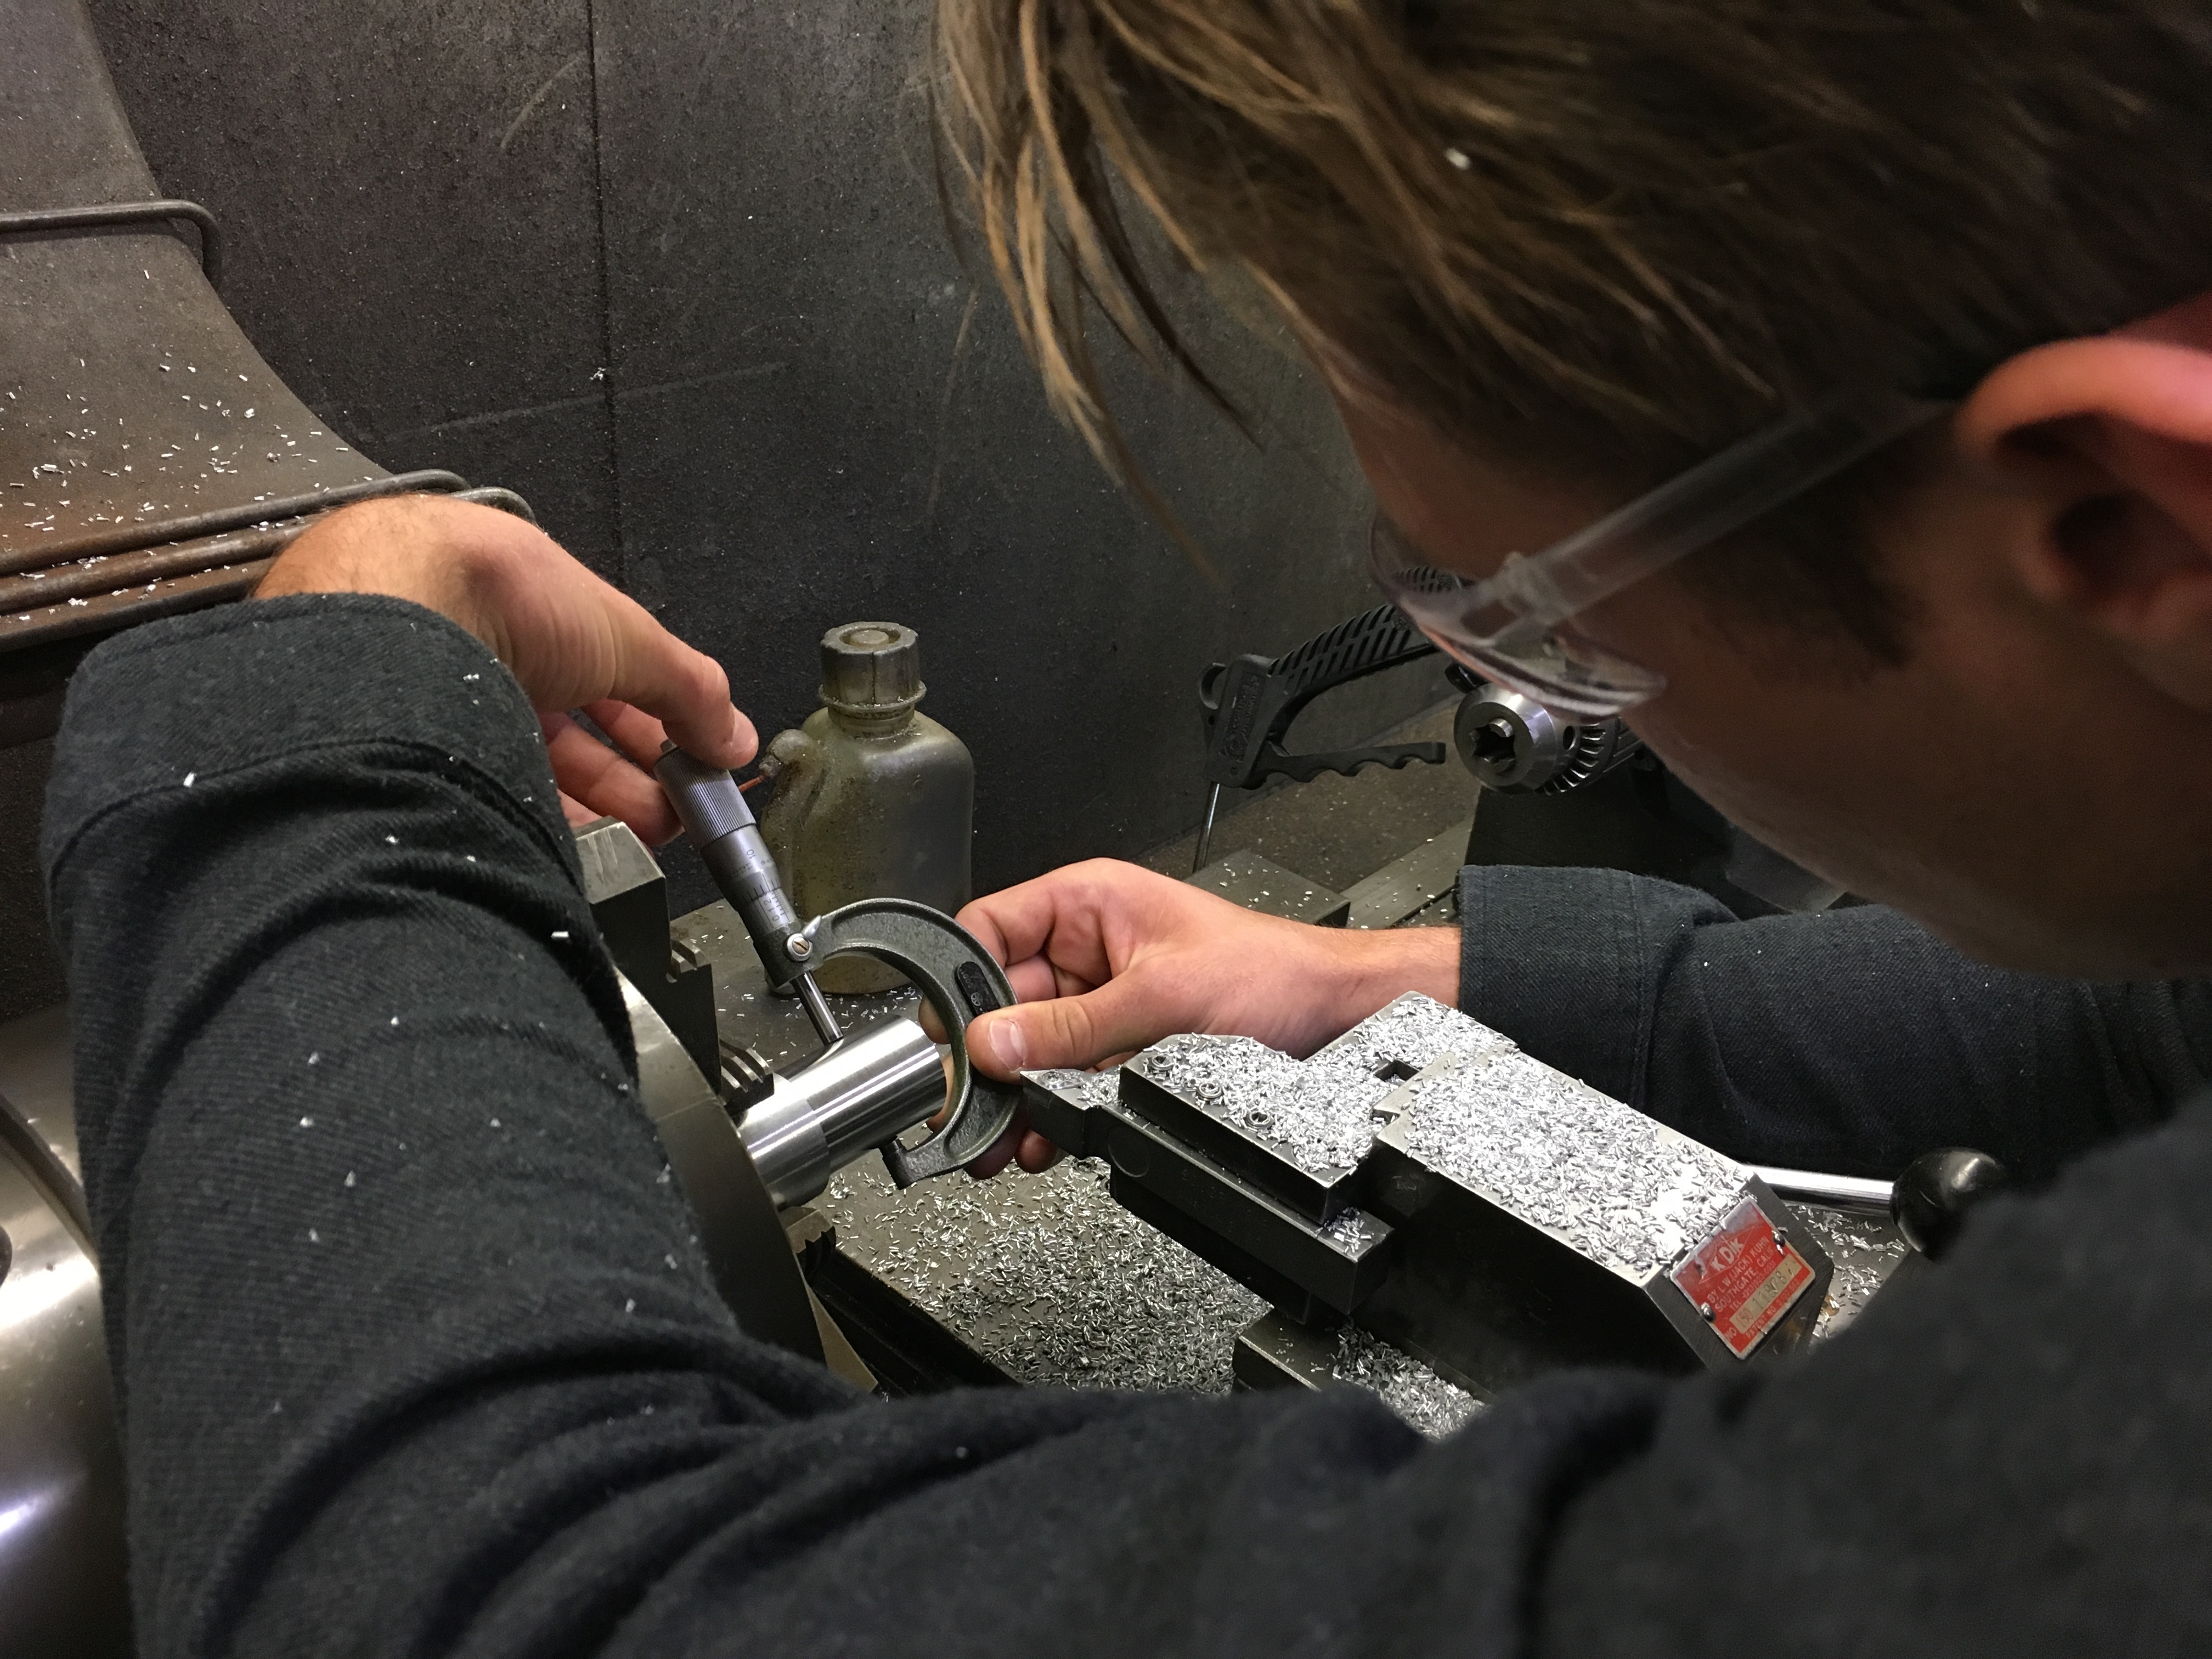
\includegraphics[width=.6 \textwidth]{08_10-22/images/IMG_0330.JPG}
    \caption{Oren checking part measurements}
    \label{fig: Turning Inserts}
\end{figure}

\clearpage \newpage \section{Week \thesection} 
\subsection{Business Goals}
\paragraph{B1: Continue work on the Business Notebook}
 Finish the budget, goals and action plan, and the finishing touches on outreach events.
\subsection{Hardware Goals}
\paragraph{H1: Print the Marker}
 Give Kelly the marker CAD to be printed.
\paragraph{H2: Fabrication}
 Start to fabricate the parts for the robot.
\paragraph{H3: Lift Fabrication}
 Lift bearing blocks.
\subsection{Software Goals}
\paragraph{S1: Change waypoint representations}
subsection {Change waypoint representations}
% Write a wrapper around roadrunner's path generation to facilitate more intuitive waypoint creation and path design
Roadrunner (ACME's motion planning and control library), is designed to be usable by any team, regardless of their drivetrain type. For this reason, the default behaviour of the path generator is to keep the headnig of the robot consistant with the direction of travel, so that the paths are executable by a tank drive robot. Spline paths are created by calling \texttt{PathBuilder.splineTo (Pose2d pose)}, where the positional component of the pose represents the location of the endpoint of the spline, and the heading component represents the direction of travel on entering the point, which in a tank drive is the same as the heading of the robot. To facilitate holonomic drives, where the direction of travel is not neccecarily, and in fact idealy is not the same as the heading, an optional \texttt{HeadingInterpolator} can be passed, which could be constant, linear, or some other sort of more sophisticated interpolator. In most cases, a linear interpolator should be used, so that a single profile can be used for the entire path, and heading will vary linearly with displacement along the path. The problem then becomes an issue of code readabilty and path creation. To go to a point, \texttt{builder.splineTo (new Pose2d (x, y, entranceDirection), new LinearInterpolator (startHeading, endHeading))} must be called. If the start heading of one endpoint does not mach the endpoint of the last, a heading discontinuity results, making things tougher. Points with different entrance and exit directions are also more dificult to create.

To resolve this, Kelly created two new classes, a \texttt{Waypoint} class, and a \texttt{TrajectoryBuilder} class. A \texttt{Waypoint} contains a Pose2d to store the position of the robot at the Waypoint, as well as the entrance and exit angles of the waypoint. This allows a waypoint to be declared as such:

 \lstinline{ Waypoint SAMPLE_RIGHT_DEPOT = new Waypoint(new Pose2d(48, 24, -PI / 4), PI / 4); }

The entrance and exit poses required by Roadrunner's path generation can be accesed by \texttt{waypoint.getEnter()} and \texttt{waypoint.getExit()}. To construct a set of paths, a TrajectoryBuilder object is constructed, and then passed a series of waypoints. The headings are automaticaly taken care of, and multiple paths are created if the waypoints require the robot to come to a complete stop on its way to traverse them. 

\begin{lstlisting}[language=Java]
public TrajectoryBuilder to(Waypoint waypoint) {
	currentPath.splineTo(waypoint.getEnter(), new LinearInterpolator(lastWaypoint.getHeading(), waypoint.getHeading()));
	lastWaypoint = waypoint;
	if (waypoint.getStop()) {
		trajectories.add(new SplineTrajectory(currentPath.build()));
		currentPath = new PathBuilder(waypoint.getExit());
	}
	return this;
}
\end{lstlisting}

\newpage
\subsection{B1: Continue work on the Business Notebook}

It was very important to the team to print the Business Notebook at least 24 hours before the team left for the tournament. This meant that in order to meet that goal most of the big stuff that needed to be put into the Business Notebook (budget, goals and action plan, etc.) needed to be done quickly. Emma worked on writing up these things in the BN this week. First, she finalized the budget with the other team captains and mentors and added a few additional expenses such as the cost of the field. Then she put all of this information into a table that could be easily read and understood. For the goals and action plan Emma worked with Stephanie to come up with a new way to display the team's plans for the future. Basically, each goal is listed and given a short summary, then the plans to meet that goal are written in bullet form and then several paragraphs below that illustrate how the team is working to complete the goal or the results of that plan. Emma also added a section to the outreach events about future events that the team is planning. Such events include a presentation to the local Girls Who Code club, a meet up with a VEX robotics team in the county and a workshop with the Girl Scouts. (For more information on these events and other outreach events, please peruse the Business Notebook). \subsection{H1: Print the Marker}

This week Ben finished revising the model of the team marker in Inventor Pro 2018. He then converted the .iam file to an .stl file to be printed. Then, he gave Kelly the file to be printed. Towards the end of the meeting, Ben tapped about 10 churros to be used in the drive train. Figure \ref{fig:marker} shows the final marker. 

\begin{figure}
    \centering
    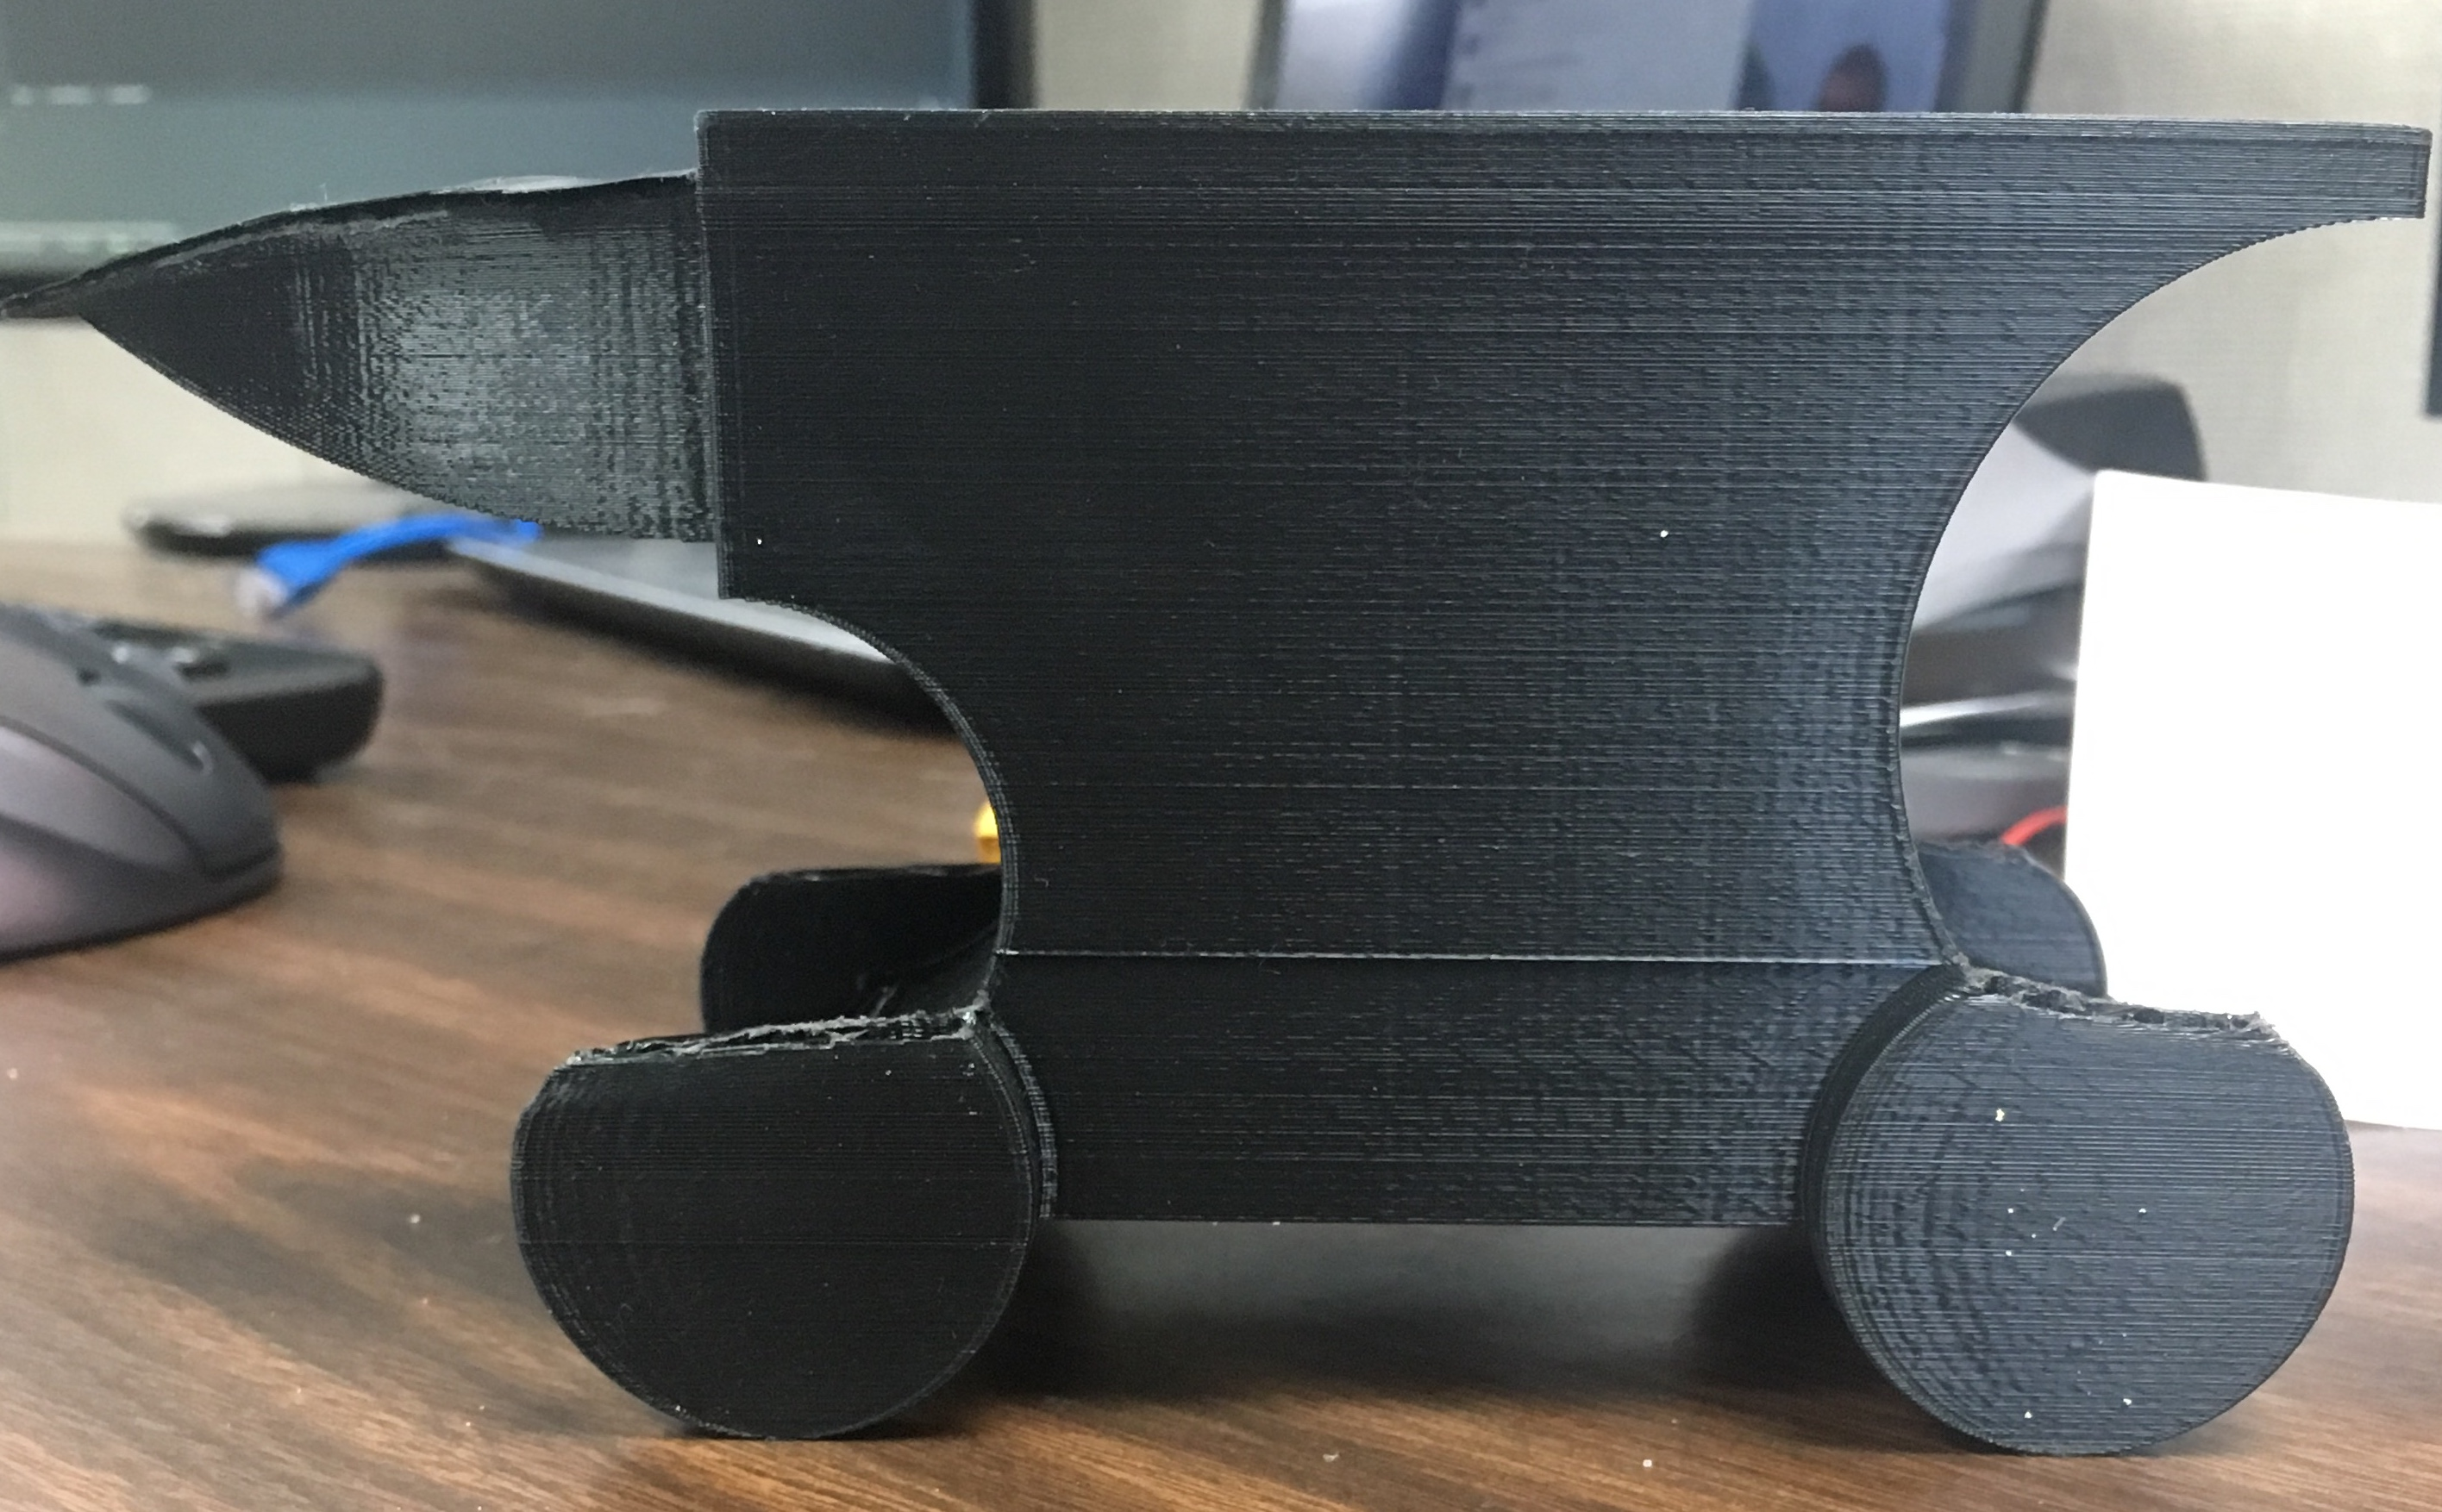
\includegraphics[width=.6 \textwidth]{09_10-29/images/anvil_marker.jpg}
    \caption{Anvil Marker}
    \label{fig:marker}
\end{figure}

\subsection{H2: Fabrication}

Now that the team had most of the parts of the robot, they could begin fabricating the robot. To assemble the intake and drivetrain, the metal cross beams and Vex rollers needed to be cut down to size. Jon had a chop saw and band saw at his house so he took the Vex rollers and cross beams home to be cut. To complete the rollers for the intake, holes had to be drilled in the rollers for the surgical tubing. After drilling a test piece, Jon had to rearrange the way the rollers were clamped in the vice. He then drilled the rest of the Vex rollers.

\begin{figure}
    \centering
    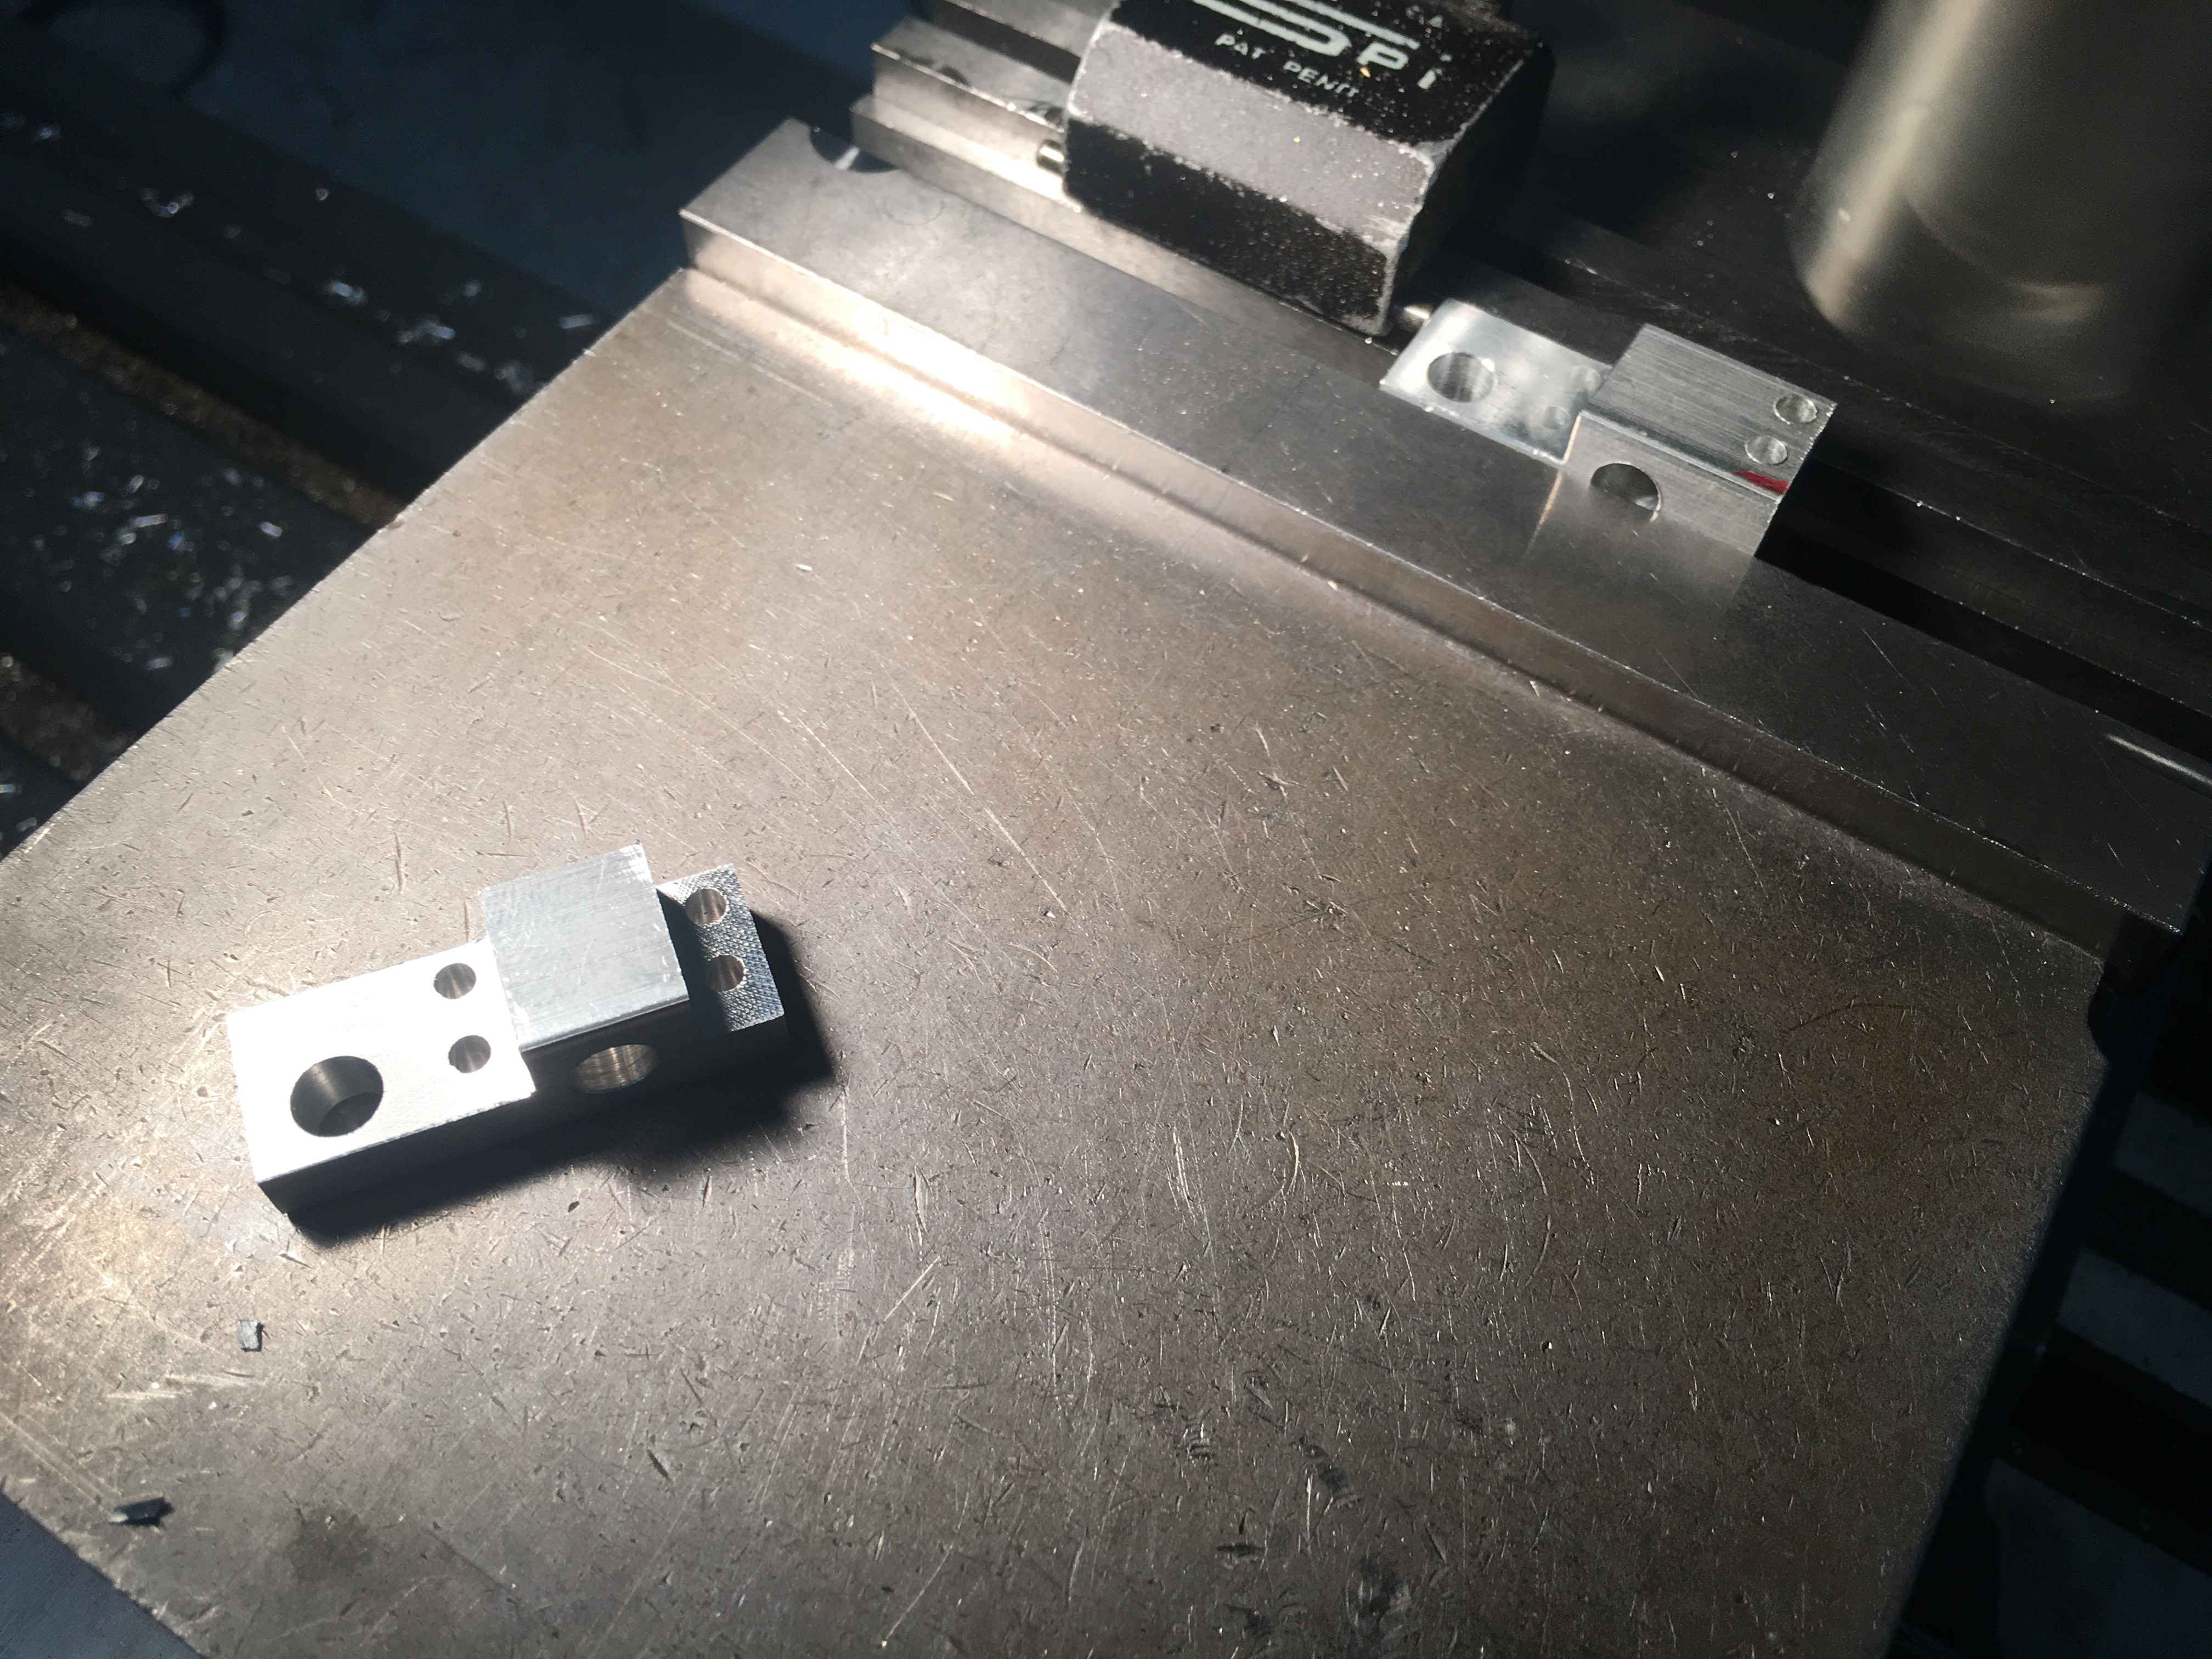
\includegraphics[width=.6 \textwidth]{09_10-29/images/bearingblock.JPG}
    \caption{Bearing Block}
    \label{fig:bearingblock}
\end{figure}


\subsection{H3: Lift Fabrication}

Oren went to GSS a sponsoring company to work with a one of there mechanical engineer, on milling custom bearing blocks for the lift. The team this year wanted to custom fabricated a lift that would be robust enough to hold and lift the in both the the beginning and end of the match. 
\subsection{S1: Change waypoint representations}

\clearpage \newpage \section{Week \thesection} 
\subsection{Business Goals}
\paragraph{B1: Add finishing touches to the Business Notebook}
 Finish the Appendices and do a final read through of the Business Notebook.
\paragraph{B2: ACME Board}
 Finish the pit board that the team is going to take to the Burlingame tournament.
\subsection{Hardware Goals}
\paragraph{H1: Sorter Finalization}
 Complete last edits to the sorter.
\paragraph{H2: Intake shield}
 Manufacture and make intake shield.
\paragraph{H3: Drivetrain Assembly}
 Assemble the drivetrain.
\subsection{Software Goals}
\paragraph{S1: Investigate problem with motion profile generation}
 Investigate a problem that causes trapazoidal profiles to be returned instead of s-curve profiles in some cases.
\newpage
\subsection{B1: Add finishing touches to the Business Notebook}

The final part of the Business Notebook was writing the Appendices. The Appendices are very important because they include all of the extra information that doesn't fit other sections in the notebook. For example the fundraising letters are put in to the appendix because they are very long and don't fit perfectly in the section where fundraising and sending the letters is mentioned. Therefore, they are referenced in those places but the real letters are at the back of the notebook. This is the same story for the budget details. There is a general budget in the budget section but the individual purchases are in the appendix. \\
The final thing to do with the BN is to read through it once more, fix typos, add a few more photos and print the notebook. Emma took team and mentor photos for the bios and then a team photo for the "team" section. After that was done, she downloaded the BN PDF and printed the notebook. There are still a few things to add in order for the notebook to be completely done, such as write the summary page and space out the sections with dividers, but the goal to print the notebook at least a day before the tournament was met!

\subsection{B2: ACME Board}

This week, Ben was tasked with making the ACME board. To do this he typed up multiple short paragraphs about subsystems, outreach, and software. Then he printed them out along with photos that show a visual. In Figure \ref{fig:pitboard} you can see the sketch that Ben made of the layout of the board. 

\begin{figure}
    \centering
    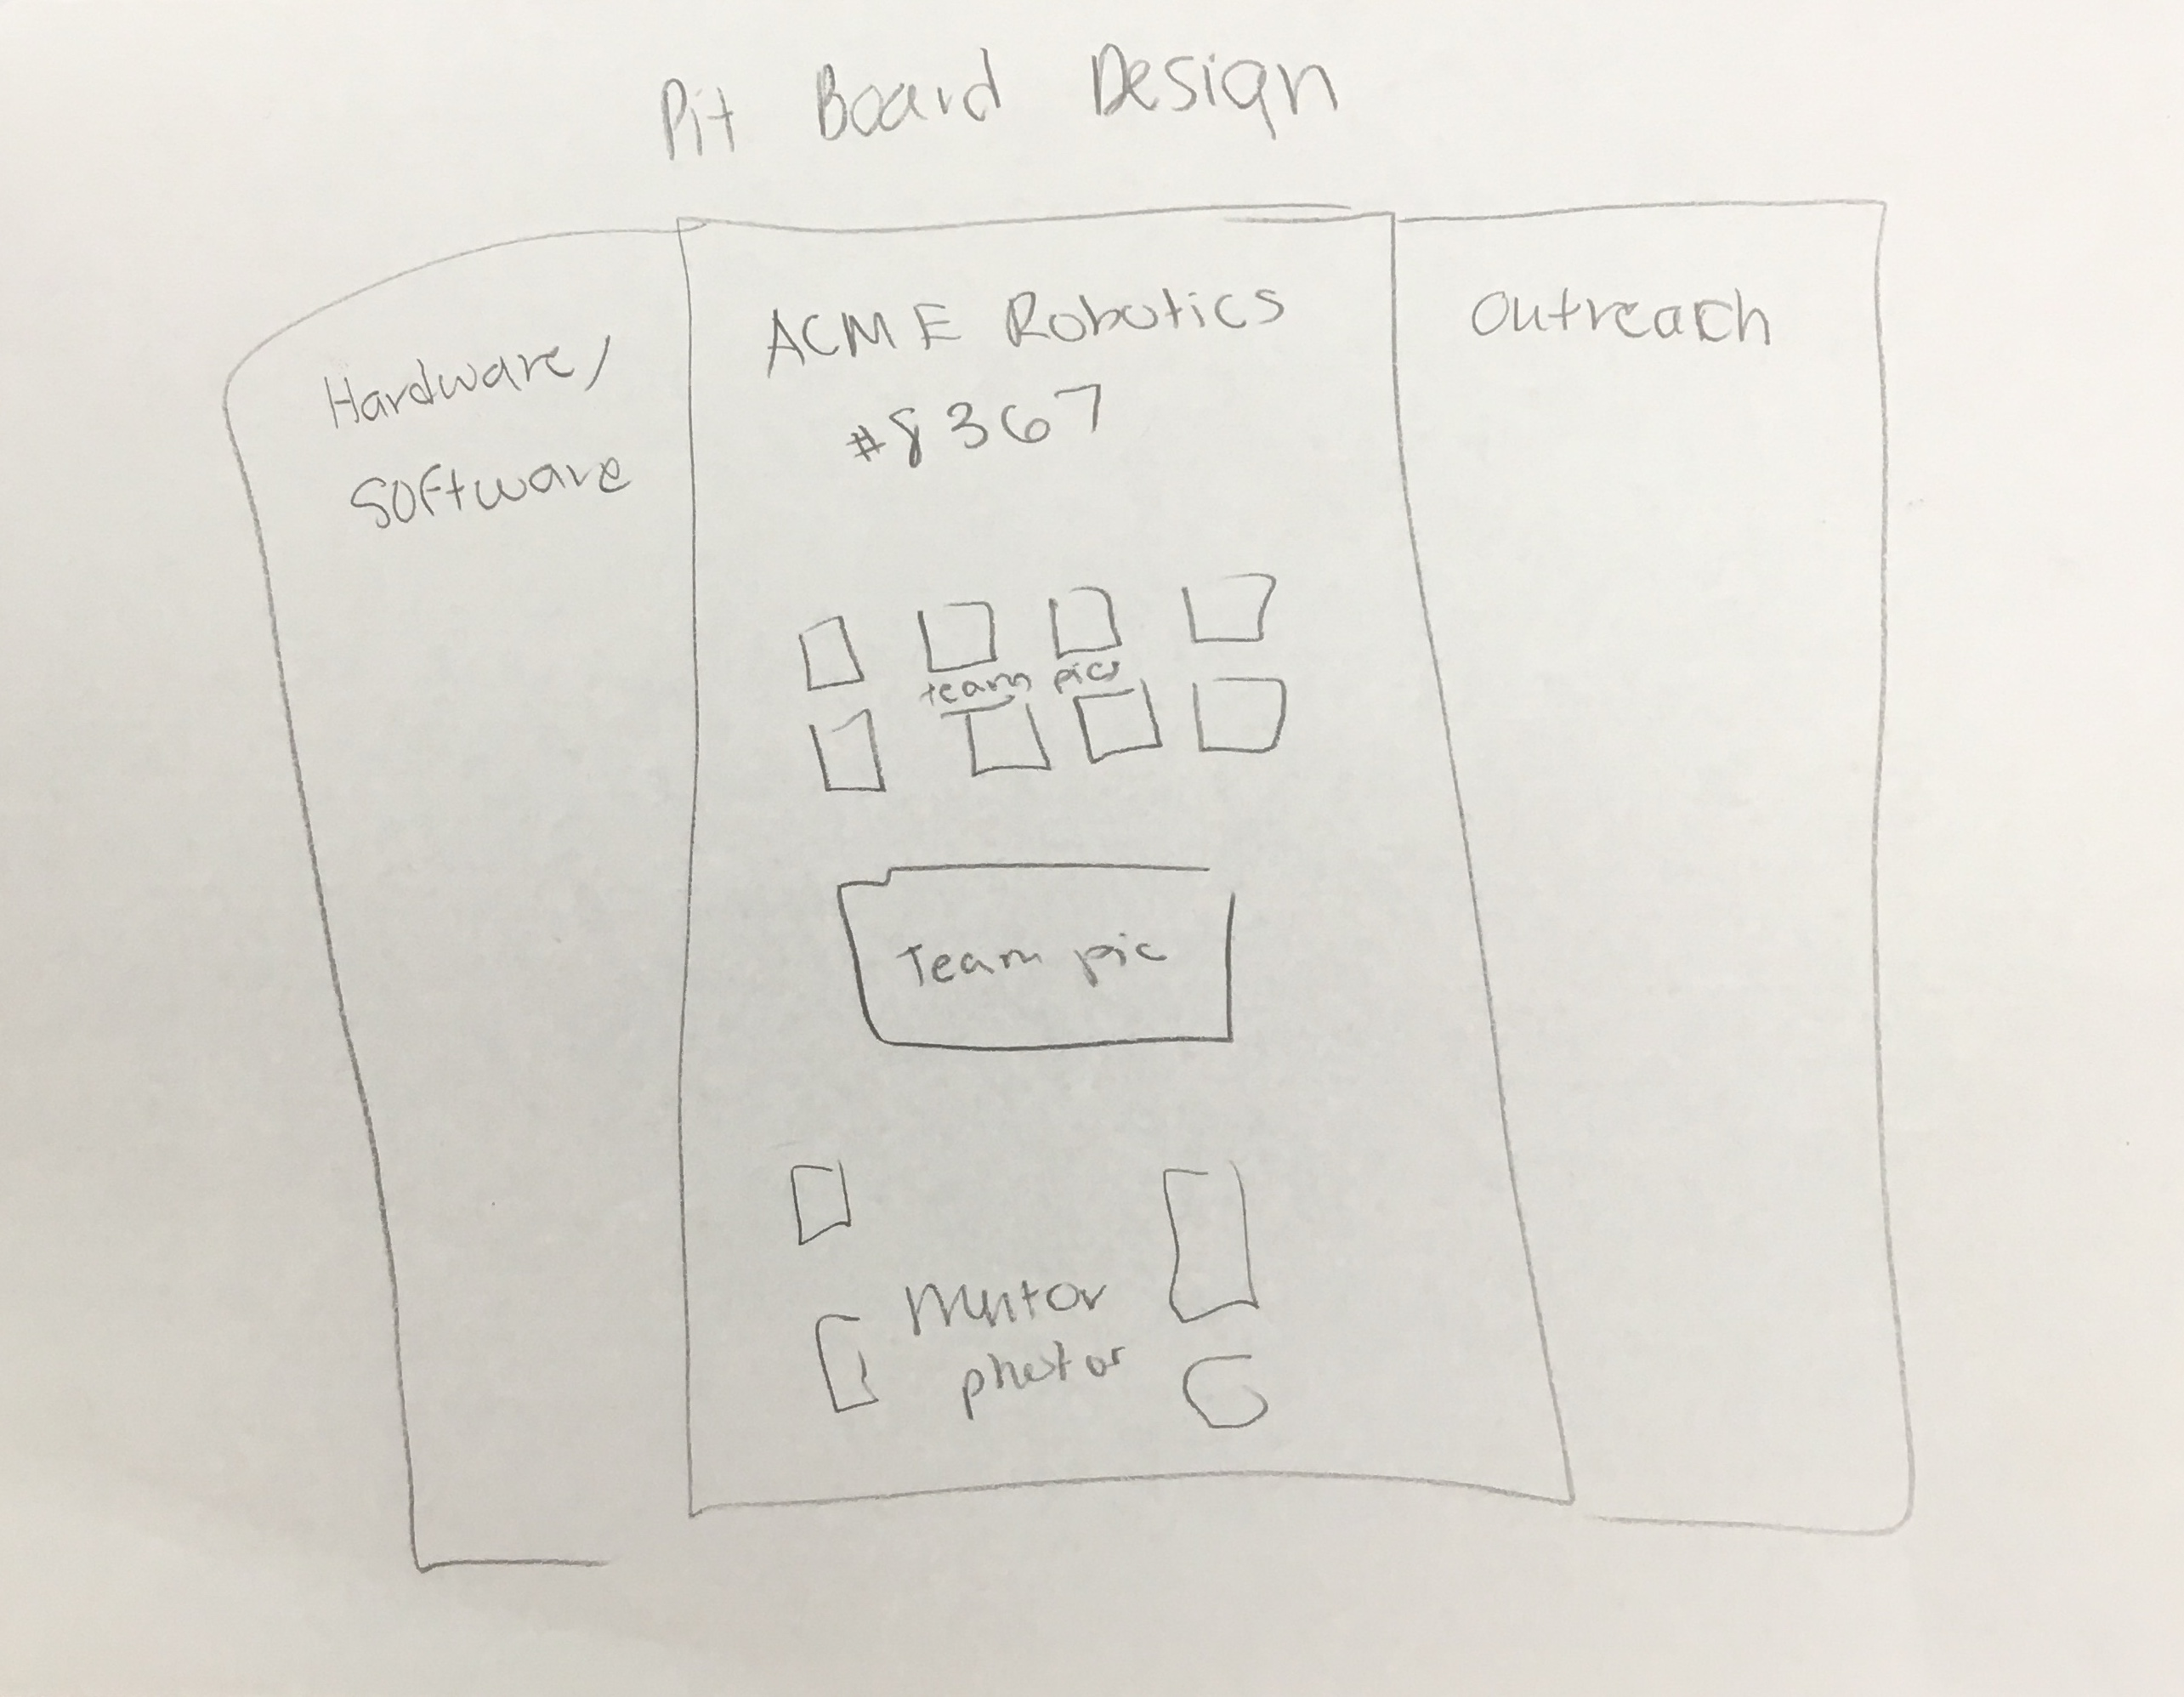
\includegraphics[width=.6 \textwidth]{10_11-05/images/pit_board.jpg}
    \caption{Pit Board Sketch}
    \label{fig:pitboard}
\end{figure}
\subsection{H1: Sorter Finalization}

The sorter needed to be printed as soon as possible so Ashlin and Aidan made some finalizing touches to the sorter so that it could print. First they split it the base design into two parts making the top be its own piece. They did this so that the top could be removed to allow for the swiveler to be put in the sorter and also so that the top piece could be printed separately to allow for the print to be easier. They also edited the top piece so that a bearing could fit into it tightly which would allow for the overall rotation of the sorter to be that much smoother. They printed the sorter on one of their sponsor's printers (see Figure \ref{}).

\begin{figure}
    \centering
    \includegraphics[width=.6 \textwidth, angle=270 ]{10_11-05/images/sorter.JPG}
    \caption{Sorter and Intake CAD}
    \label{fig:Intake CAD}
\end{figure}

\subsection{H2: Intake shield}

After the intake shield was cut Ashlin and Aidan heat bent the shield so that it would be shaped exactly as the 3D model. After the shield was bent they tested it to make sure it successfully in-took balls and cubes. The testing was successful and the shield worked  spectacularly.

\begin{figure}
    \centering
    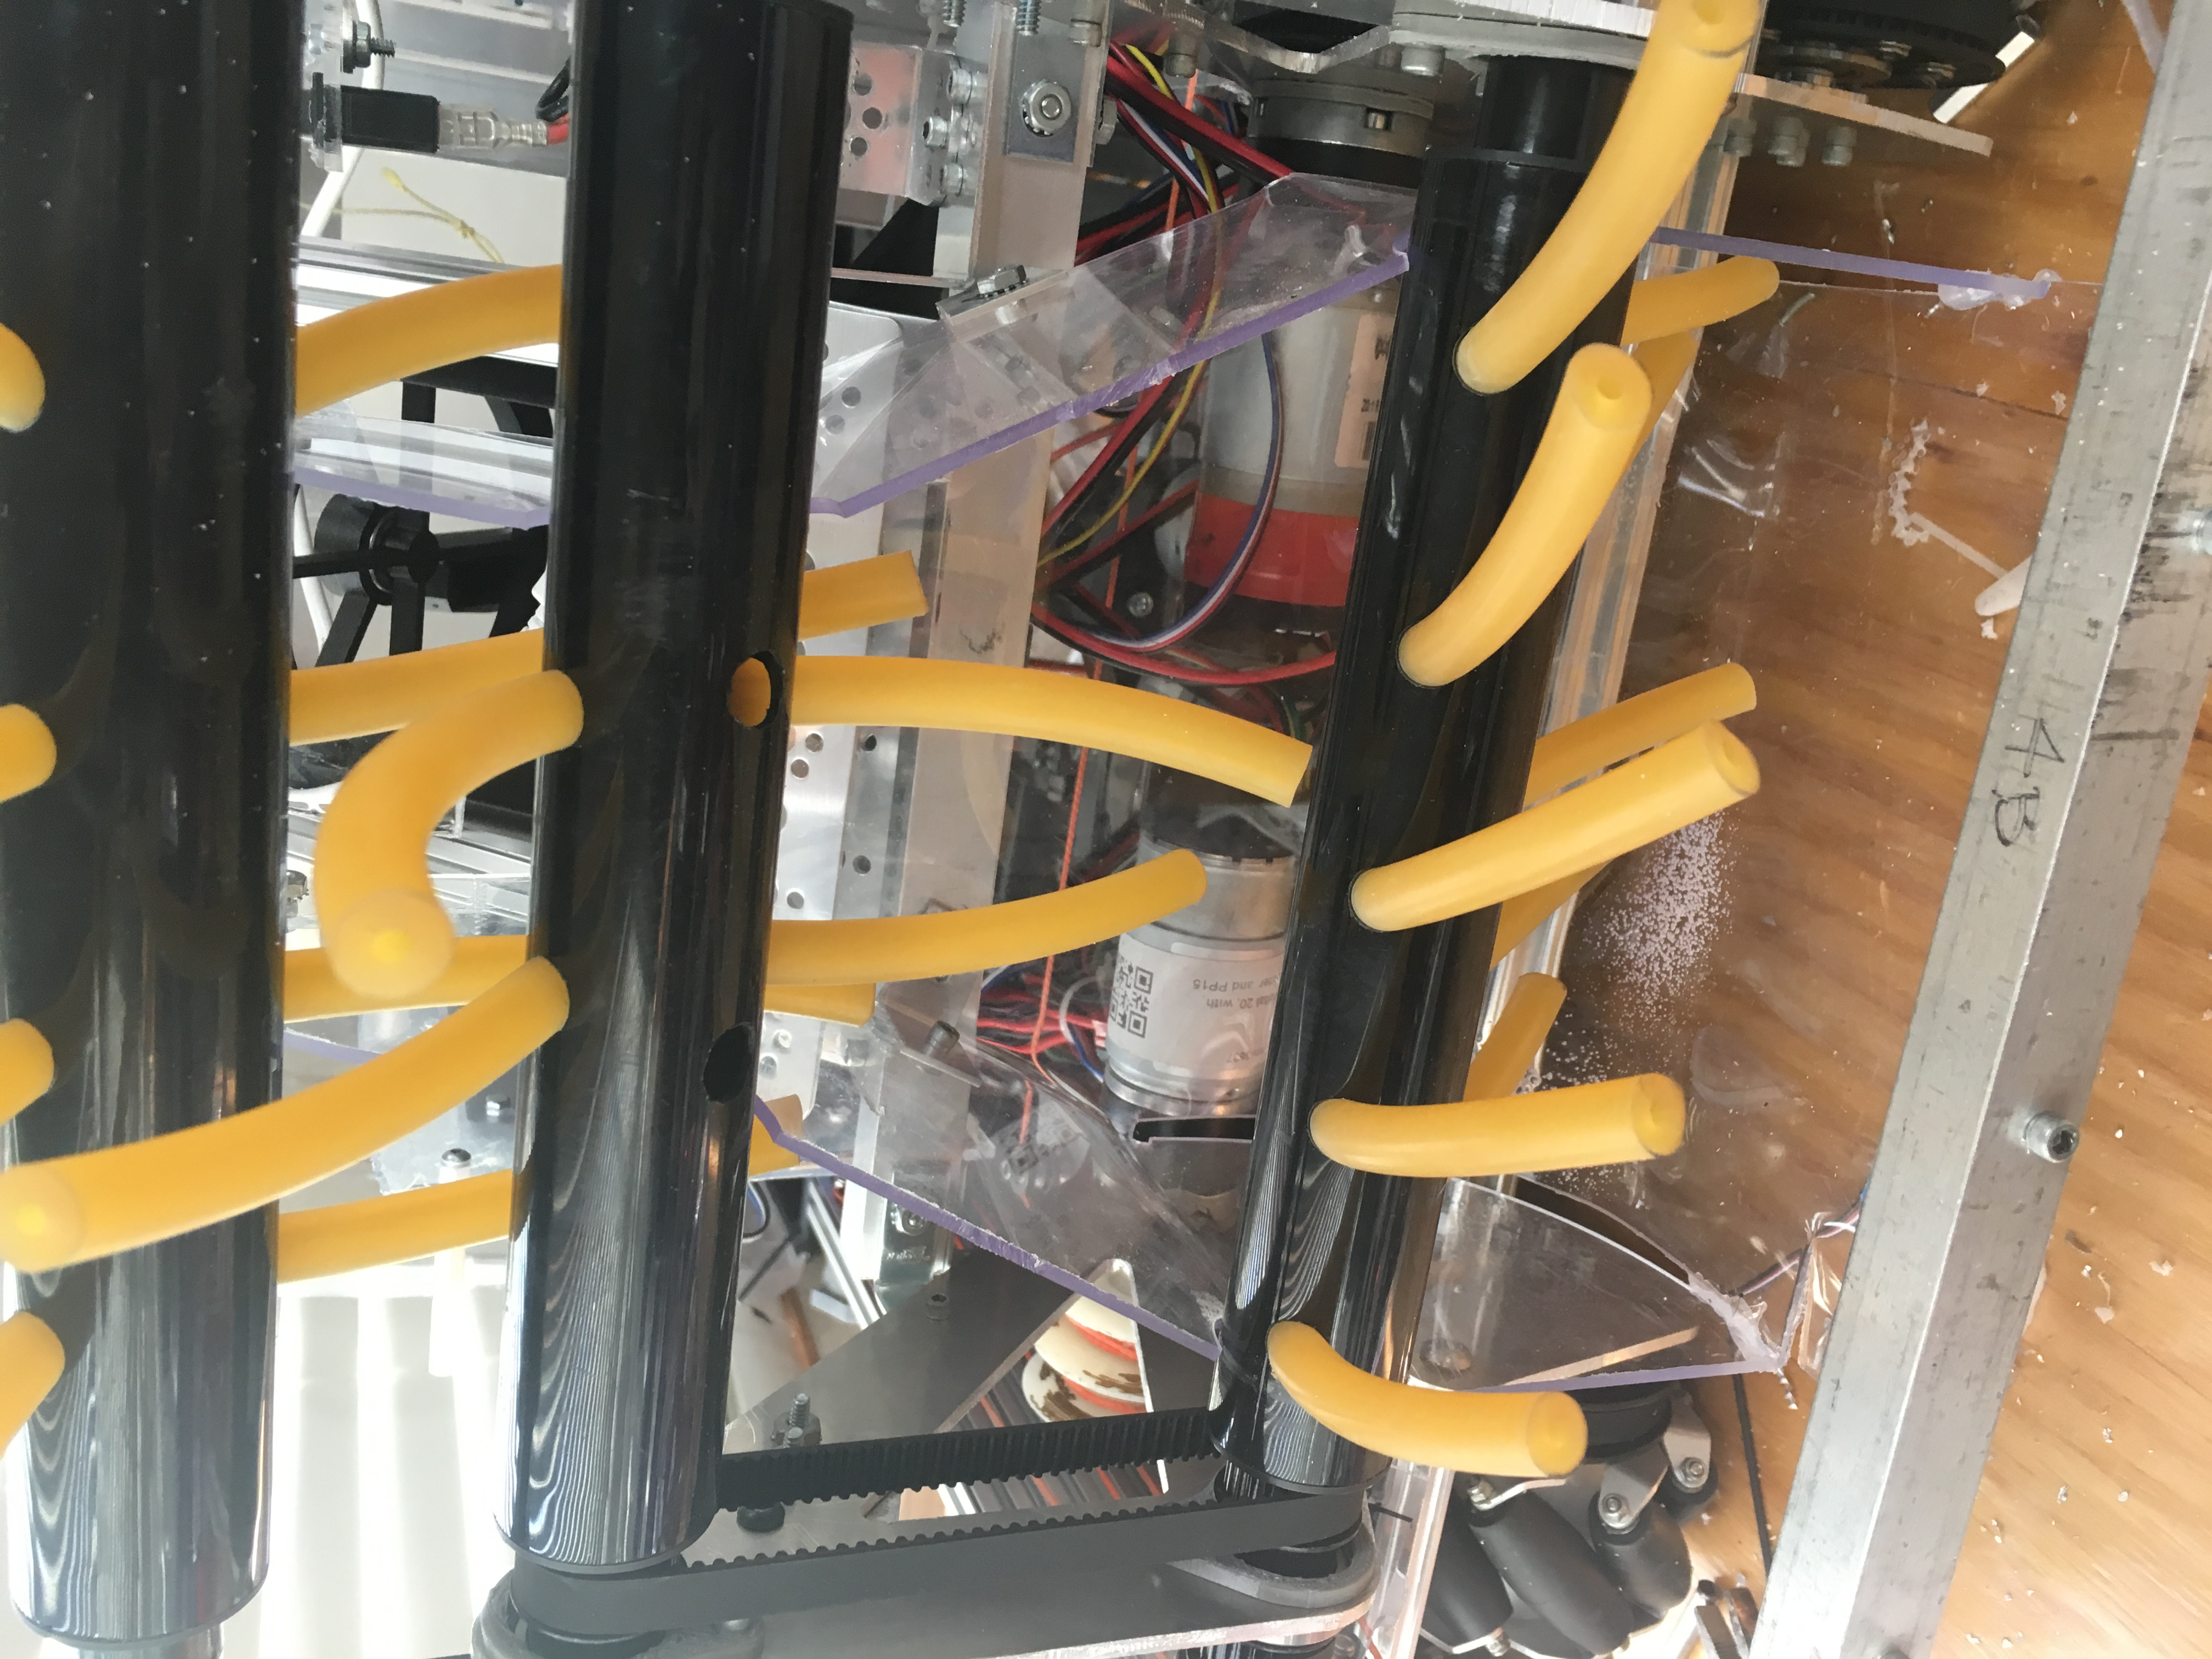
\includegraphics[width=.6\textwidth, angle=270]{10_11-05/images/intake_shield.JPG}
    \caption{Intake Shield}
    \label{fig:Intake Shield}
\end{figure}

\subsection{H3: Drivetrain Assembly}

This week Oren assembled all of the parts for the drive-train, there was some errors and misshapes. That include needed motor mounts, new more accurately cut cross members and some needed   screw holes for mounting things. The drive-train when completed functioned actually like we had planned and was very silent when running.    

\begin{figure}
    \centering
    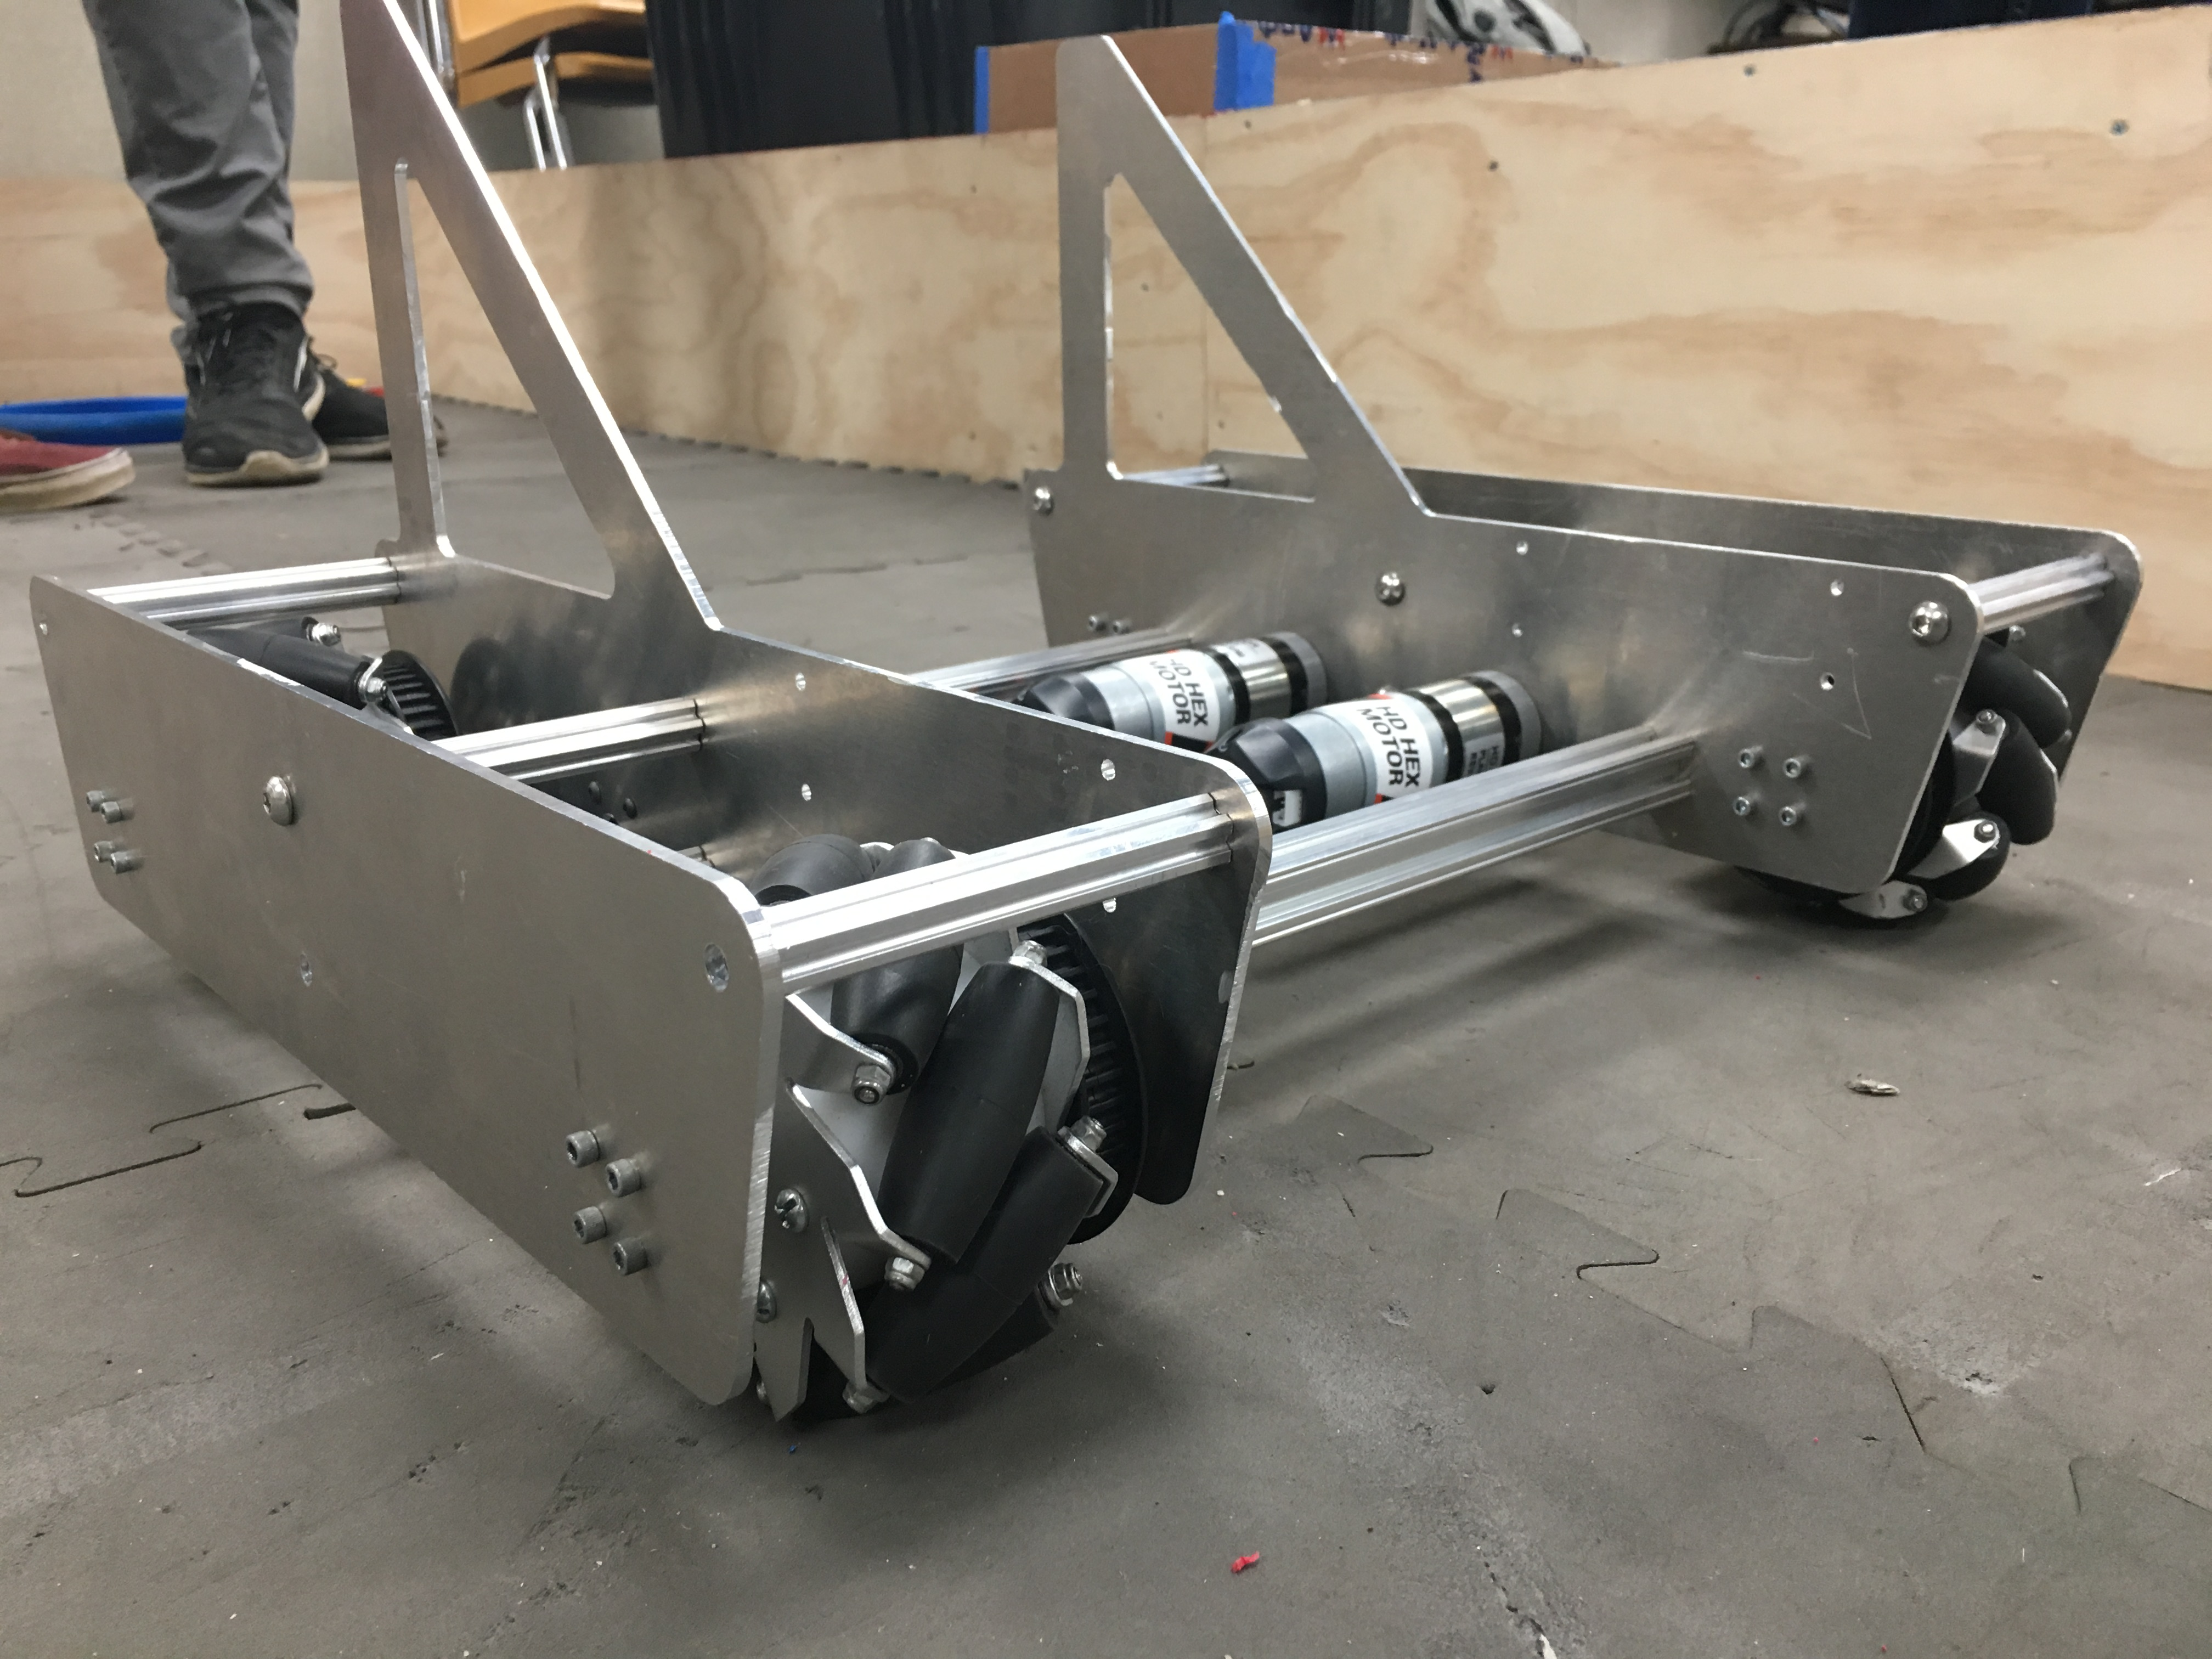
\includegraphics[width=.6 \textwidth]{10_11-05/images/drivetrain.JPG}
    \caption{Drivetrain}
    \label{fig:drivetrain}
\end{figure}
\subsection{S1: Investigate problem with motion profile generation}

While testing pathing on the robot, Kelly found that under certain circumstances a trapazoidal profile would be returned instead of a s-curve profile. This increased error significantly by attempting to instantaniously change the acceleration of the robot, and made the motors sound wierd whern there were discontinuities in their pitch caused by the acceleration discontinuities. After testing Kelly determined that the problem occured when the profile was not long enough for the robot to achieve maximum acceleration. 


\begin{lstlisting}
                var upperBound = maximumVelocity
                var lowerBound = 0.0
                var iterations = 0
                while (iterations < 1000) {
                    val peakVel = (upperBound + lowerBound) / 2

                    val searchAccelProfile = generateAccelProfile(start, maximumVelocity, maximumAcceleration, maximumJerk)
                    val searchDecelProfile = generateAccelProfile(goal, maximumVelocity, maximumAcceleration, maximumJerk)
                            .reversed()

                    val searchProfile = searchAccelProfile + searchDecelProfile

                    val error = goal.x - searchProfile.end().x

                    if (abs(error) < 1e-10) {
                        return searchProfile
                    }

                    if (error > 0.0) {
                        // we undershot so shift the lower bound up
                        lowerBound = peakVel
                    } else {
                        // we overshot so shift the upper bound down
                        upperBound = peakVel
                    }

                    iterations++
              }

\end{lstlisting}

In this code snippit, a binary search is used to compute the max velocity that will be reached in the case that the robot does not have enough time to reach its actual max velocity. This algorithm had been working last year, but when it was re-written in Kotlin over the summer in preperation for the public release of roadrunner, a mistake was made in these two lines:

\begin{lstlisting}
                    val searchAccelProfile = generateAccelProfile(start, maximumVelocity, maximumAcceleration, maximumJerk)
                    val searchDecelProfile = generateAccelProfile(goal, maximumVelocity, maximumAcceleration, maximumJerk)
                            .reversed()
\end{lstlisting}

Rather than generating the search profiles with \texttt{peakVel}, the valiable whose correct value is being searched for, the profiles were generated with \texttt{maximumAcceleration}, the constant constraint used to generate all the profiles. This meant that the search profile never actualy changed, so the thousand iterations of the search would be preformed to no avail, and then a backup trapazoidal profile returned. By changing those two  lines to generate the search profile using \texttt{peakVel} instead, the search would converge to within $10^{-10}$ in around thirty iterations, the same preformance as last year. 

\clearpage \newpage \section{Week \thesection} 
\subsection{Business Goals}
\paragraph{B1: Write the summary and cover pages for the Business and Engineering Notebooks}
 Finish up the BN by printing the summary and cover pages.
\subsection{Hardware Goals}
\paragraph{H1: Assembling Rev Linear Motion Slides for the Rake}
 Assembling and Attaching the Linear slides and Rake system.
\paragraph{H2: Shield Attachment}
Attaching the shield to the robot.
\newpage
\subsection{B1: Write the summary and cover pages for the Business and Engineering Notebooks}

As the tournament draws closer, finishing the Business Notebook becomes ever more important. Even though the notebook itself was already printed, a cover page and summary page was still needed to complete the task. Emma worked on the summary page this year. The summary page is not only an introduction to the team's mission, it is where specific parts of the notebook worth noting can be found, as well as specific events. Emma adapted the summary page the team used last year by rewriting the team's story and mission for this year, altering the season highlights, and choosing specific topics of interest in the notebook. The season highlights are notable events that are exciting or great accomplishments of the team. The team's overlying goal for this year is to maintain the FIRST program in our community and train members on our team so that ACME can keep going in the future. The summary also mentioned goals on how the team wants to progress to Worlds again this year. With these things complete, the BN is now complete.  


\subsection{H1: Assembling Rev Linear Motion Slides for the Rake}

Continuing the manufacturing process, Jon and Aidan assembled the linear slides for the intake rake. The team wanted to create a four stage slide so that no matter where the robot was around the crater it could reach every cube or ball in the crater. However the team had only bought two linear slide kits which would only allow for a two stage slide. John and Aidan found extra parts from the previous years linear slide system. This allowed for there to be a three stage system which would give them enough length to reach to almost the back of the crater and get plenty of minerals. After constructing the slides, Jon and Aidan had to fine tune them to get them both to run smoothly and with little resistance because there was only going to be one motor powering both slides and if there was too much resistance the motor wouldn't be able to power them. After these were constructed, Aidan went on to build the rake portion of the slide and Jon attached the slides to the robot. Jon did this by using Tetrix L brackets and screwing them into the outside plate of the drive train. This made sure the slides were inside the 18 inches and were firmly attached to the robot in case they got bumped by another robot during competition. To create the rake Aidan needed to find a way to minimize the length it added to the robot. The rake had to sit low enough so that it could tuck under the intake system but it needed to be high enough so that it would pass over the crater wall. Aidan solved this by having the axle of the rake sit exactly 4 inches above the ground.

\begin{figure}
    \centering
    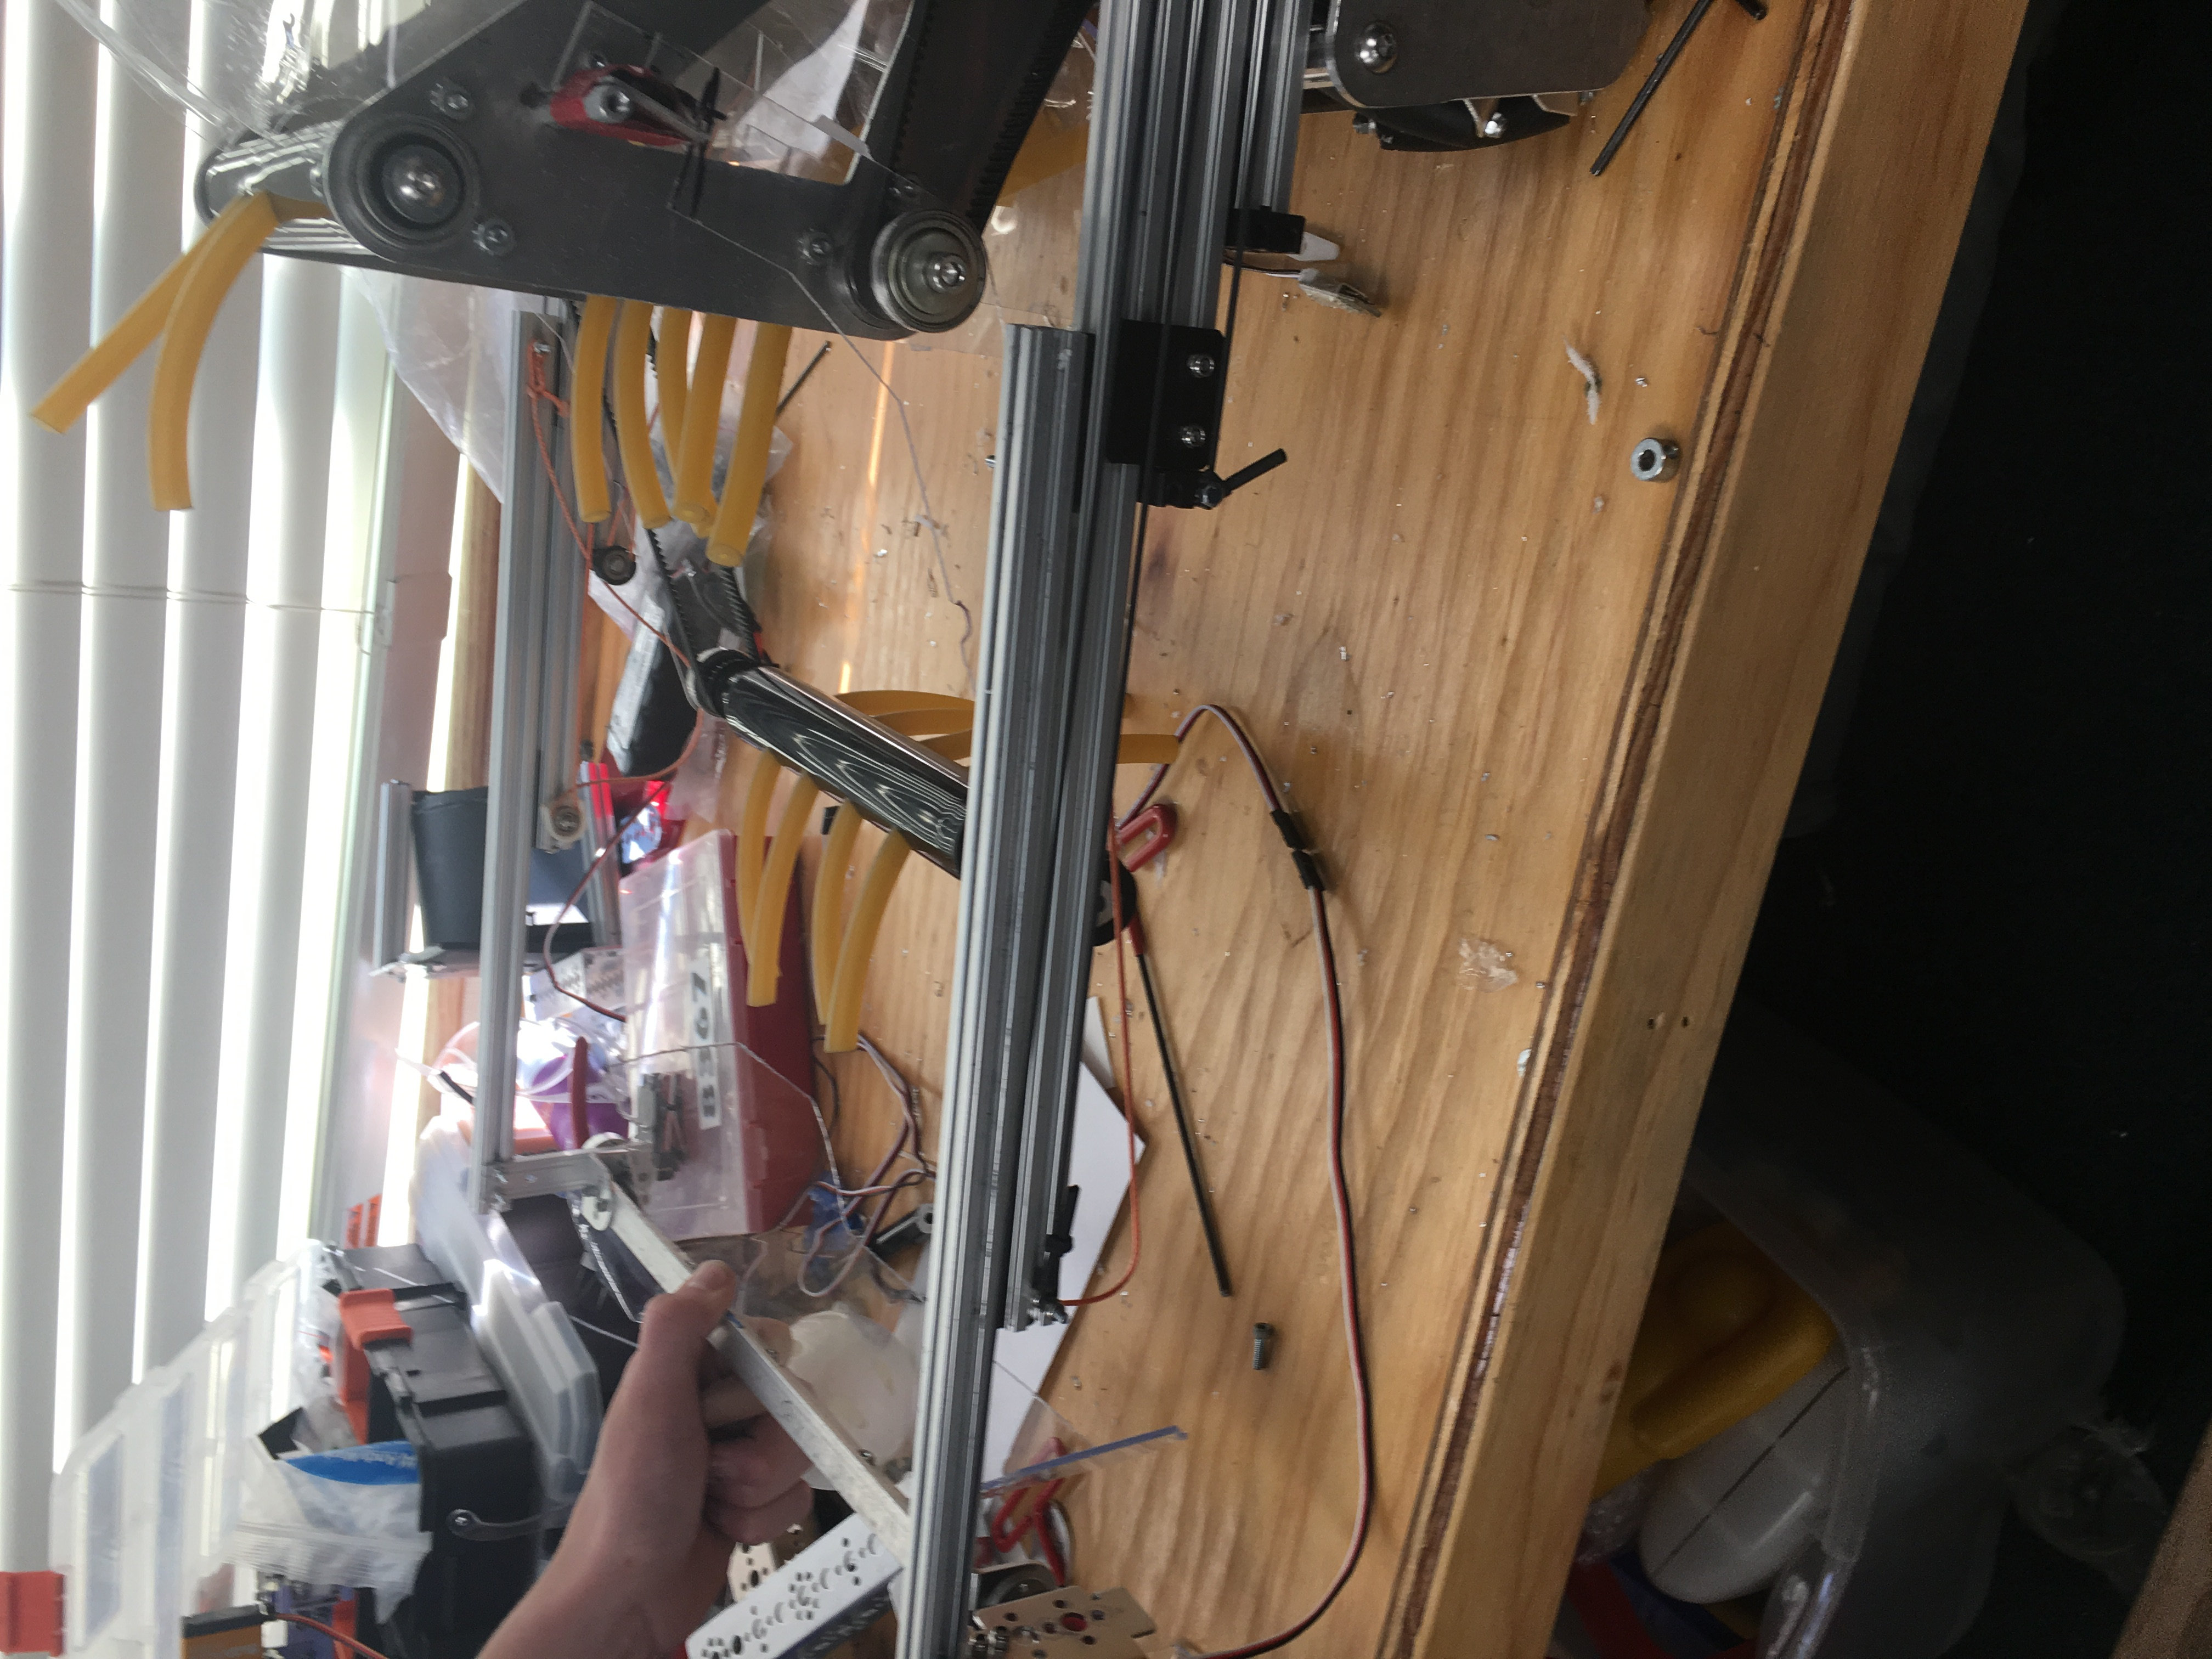
\includegraphics[width=.6 \textwidth, angle=-90 ]{11_11-12/images/rake_slides.JPG}
    \caption{Rake and Slides}
    \label{fig:Intake CAD}
\end{figure}

\subsection{H2: Shield Attachment}

After the shield was built it needed to be attached to the robot. The attachment piece would attach to the side plates of the intake But couldn't attach to the back of the sorter because the screws on the attachment might catch cubes when the went up the intake. To solve this Aidan created brackets that would allow the attachment piece to screw into the shield on the sides which would decrease the likely-hood of cubes getting caught.

\begin{figure}
    \centering
    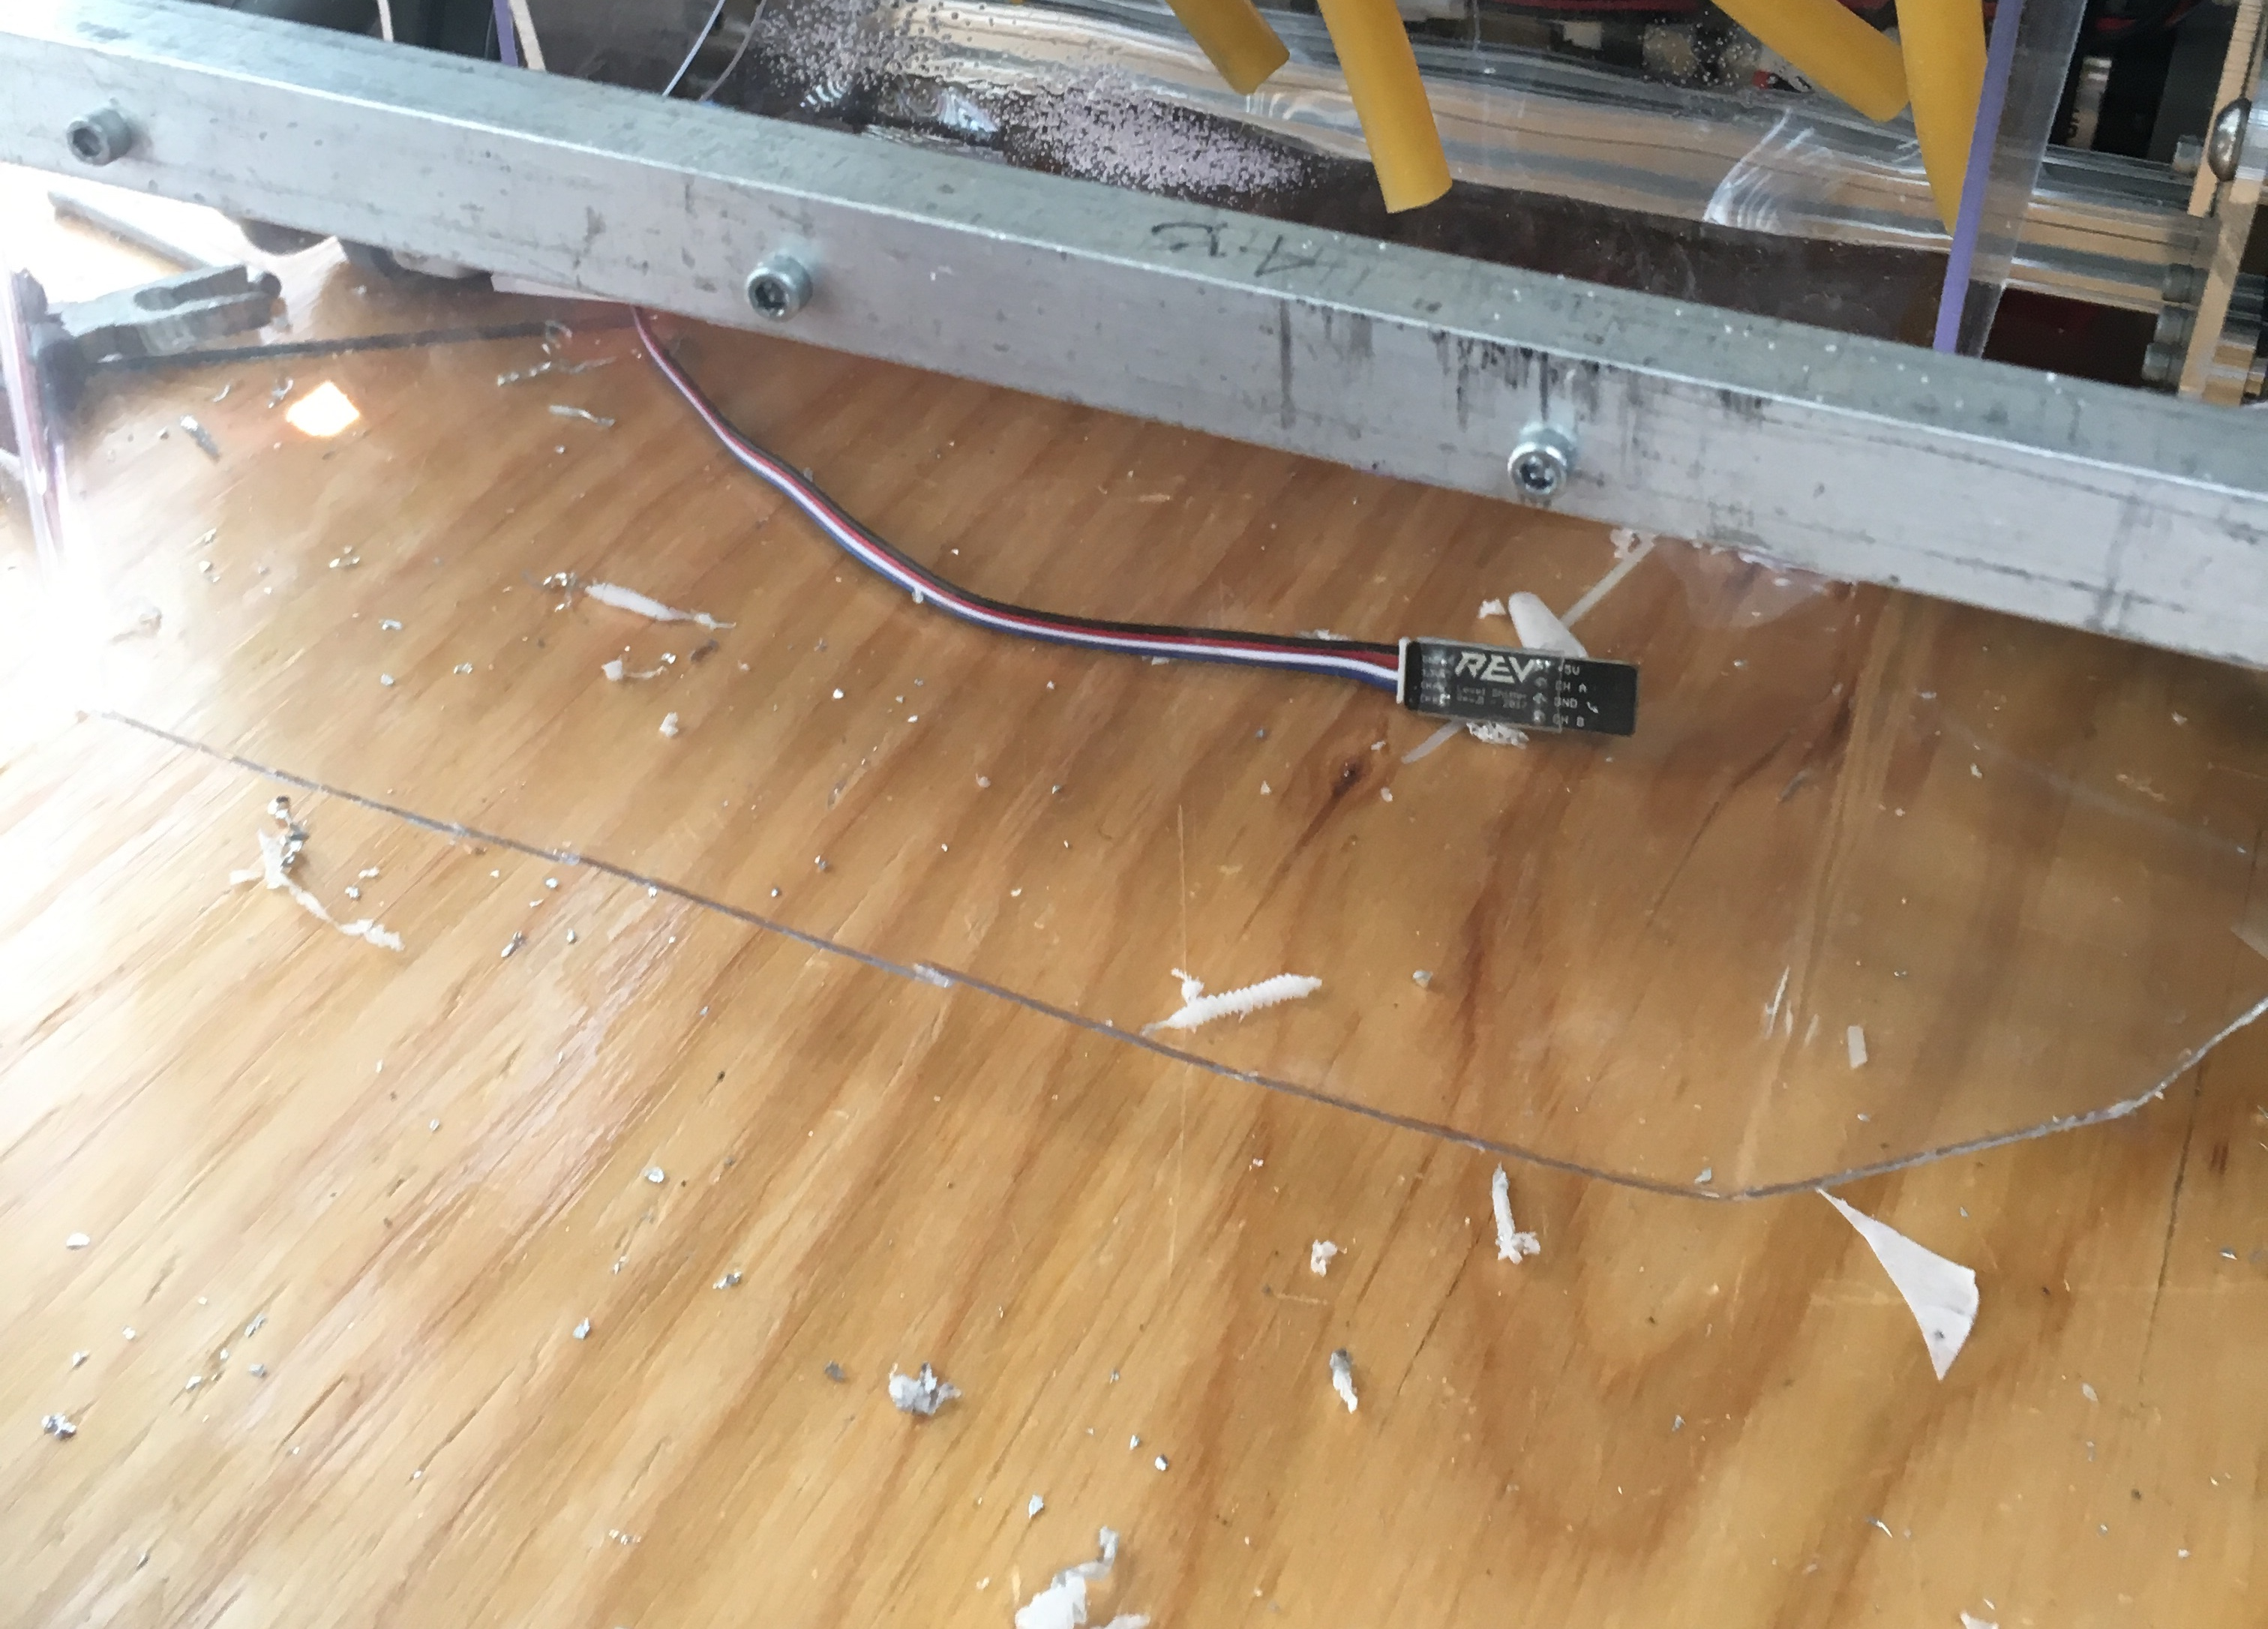
\includegraphics[width=.6 \textwidth]{11_11-12/images/rake.jpg}
    \caption{Rake Shield}
    \label{fig:rakeshield}
\end{figure}\clearpage \newpage \section{Week \thesection} 
\subsection{Business Goals}
\paragraph{B1: Attend the Burlingame Qualifier}
 Go to the Burlingame qualifying tournament to compete.
\paragraph{B2: Post Match Retrospection}
 Have a retrospective with the team for the Burlingame tournament.
\newpage
\subsection{B1: Attend the Burlingame Qualifier}

This weekend, ACME Robotics attended the Burlingame qualifier. This was their first qualifier of the season and they were looking forward to seeing other robots teams had come up with, seeing how their robot performed and whether or not they would need to rethink their strategy for the next tournament.\\

The day began bright and early at 8 o'clock. The team arrived at the venue and set up their pit. Their pit had a poster board that Ben and Shawn had made, a huge collection of ACME wristbands and, of course, RedVines. ARES, ACME's sister team was also attending this tournament. This was their very first tournament and they were looking forward to seeing what competition was like. \\

Next, the team prepared for their judging session. This was the first time Jon, Ashlin and Aidan had ever been to judging. Each team member had a talking point: Ben gave the intro, Jon and Aidan talked about outreach, Oren, Shawn and Ashlin discussed hardware and Emma and Kelly explained software. Judging went really well for them. The judges were engaged in their process and acknowledged their original and custom robot design, even if it wasn't entirely functional. They had really good questions and even gave the team time to talk about what they thought was unique about the team. \\

Judging had put everyone in an excellent mood and Oren and Emma prepared for inspection. ACME notoriously never passes inspection for the first time, mainly due to not fitting inside of the 18. The team made it a goal for this tournament to pass both robot and field inspection the first time. Both went off without a hitch and qualifying matches began after opening ceremonies. \\

As the team had such a complex robot design, they did not get it all done before the tournament. They had to rethink their strategy in order to even have a robot that could potentially score. Because of this, software didn't get the robot until that morning and they were rushing to have software to compete with. With matches about to start, the team had to make a quick decision: sit out the first match to have more time to work on the robot or put the robot on the field to see what would happen. The captains decided to allow more time to work on the robot and Emma went to the match as the team representative. This was a slight downer for the team, as it cost them a match, but they agree now that it was the right thing to do. \\

After several more matches, that the team did put the robot on the field for, judges started to come around. Three groups of judges talked to the team: control, design and connect. Each of the captains had a chance to talk to the judges more about their subteam and all three of the interviews went off without a hitch. \\

At the end of qualification matches, ACME placed 20th and ARES 18th. ACME was super proud of ARES and their performance. A few team members had to go home to work on homework, but a few stayed to watch finals and for the awards ceremony. The team was nominated for two awards, Control and Connect, which they were very proud of. However the best surprise came when the final awards winner was announced. ACME had won the Inspire Award! The team had never qualified for the Northern California Regionals at the first tournament and were very honored and relieved. This meant that the team only had to worry about making the robot as perfect as possible and not have to stress about qualifying. Everyone was super excited to win this award and could not have been happier. The team is looking forward to the next competitions to come!\\

\subsection{B2: Post Match Retrospection}

After such an eventful tournament for ACME, the team had a retrospective to assess their performance. This gives ACME a good sense of what they did wrong, what they did right, and how they can improve for next time. Helping ACME to decide exactly where they want to go next with the robot and the team as a whole, and how to get there. Some of the things the team thought they did well was judging, the business notebook, and the drivetrain was very solid. Some things they thought didn’t go well was the robot wasn’t nearly as functional as it needed to be, keeping up with EN entries, and, perhaps most importantly, they didn’t where tutus! After writing down and sorting all the reflections of the various team members; the team discussed them further and created goals for the upcoming Intel tournament. Goals are essential because they give the team something to work towards as well as keeping them focused on the important tasks. Some of the goals the team is now working towards are to deploy from, and re-latch to, the lander, create a hard deadline for EN entries, and finish the scouting app to streamline scouting. Overall the team was happy with how the retrospective went and excited to move forward and improve. 
\clearpage \newpage \section{Week \thesection} 
\subsection{Hardware Goals}
\paragraph{H1: Hardware Discussion}
 Have a team-wide discussion about the next steps for the hardware team.
\paragraph{H2: Sorter Testing}
Test the sorter to see if the team needs to reevaluate the sorting process.
\paragraph{H3: Latch Design and Development}
 Design a latch to mount on the robot that will be used to latch onto the lander.
\paragraph{H4: Testing of Rev linear slides}
 Test the REV linear slides the team uses for the rake.
\subsection{Software Goals}
\paragraph{S1: Pre-Tournament Scouting Application}
 Start working on an application that will use the Orange Alliance API to get information about other teams. 
\paragraph{S2: Joystick ramping}
Experiment with joystick profiles and speed ramping.
\newpage
\subsection{H1: Hardware Discussion}

After the first competition the team's goals were reevaluated. The sorting mechanism was not functional and untested. The lift motor was not correctly mounted and its spool was causing issues. The rake mechanism for the intake used a pulley system that had a tendency to unspool and the REV friction slides were not working correctly, which resulted in each side retracting at different speeds. The team had a meeting to discuss what the next steps were. They listed priorities, such as the lift, intake and the sorting mechanism. These were the things that the team felt were vital to successfully compete in the next competition. The week was spent testing several concepts that the team didn't have time to test before the Burlingame tournament. \\

The outcome of the discussion lead to a large change in the overall placement of specific subsystems, resulting in a great deal of CAD redesign. The team ended of changing the placement of the drivetrain's cross members to allow for the correct placement of the lift-motor. The team also realized that the design could be more streamlined and compact, by adding the intake's super-structure to the drivetrain's aluminum side-plates. Along with adding mounting holes for the subsystems that was not previously foreseen.  \\


\subsection{H2: Sorter Testing}

Aidan took on the project of testing the sorter. The team didn't have time to incorporate the sorter into the robot before the Burlingame tournament and still needed to be fully assembled and tested. Aidan and Ashlin tried to assemble the sorter specifically so that it would take up as little space as possible. They did this because there was limited space on the inside of the robot and the sorter, the cartridges, and the lift motor were all competing for this room. After fully assembling the sorter and testing the the team decided it took to much room and they wouldn't pursue it any further.

\subsection{H3: Latch Design and Development}

Ben and Shawn designed the latch to make the robot hang. They used a design where, if the robot was fully turned off, the robot would still latch. They designed it so that the servo pulls the axle back so they robot isn't latched anymore. They then prototyped this design with Tetrix and found that there were problems. Then they solved these problems and are going to try to find a way to manufacture a more professional looking latch.

\subsection{H4: Testing of Rev linear slides}

After the team's first qualifier where the rake did not function properly, ACME wanted to do some testing and see what the problem was. The rake system is crucial to ACME's current design so it was important that this was done ASAP. After Jon did some testing with the rake, he found that the problem lay with the Rev linear slides. There was too much friction in the slides and the string was spooled wrong and was causing the slides to move unevenly. He also found that the string had a tendency to become un-spooled. Jon and the rest of the team decided that removing one of the slides might remedy the problem. After Jon tested this some, he found that while somewhat better, the results where still far from satisfactory. This lead Jon to the conclusion that the Rev linear slides would have to be scrapped for some other form of linear motion. Jon then commenced brainstorming, researching, and testing for several other forms of linear motion. Nearly all the options Jon looked into did not fit for what ACME had in mind. For example, drawer slides were too heavy could not reach far to far crater wall. One that did look promising however was X-Rail. Jon thought X-Rail looked promising because it was similar to the Rev linear slides in function but could carry more weight, were sturdier, and used running bearings (making them smoother and removing friction). This made X-Rail the most practical and simple option. After presenting his findings to the team, ACME decided to give X-Rail a try. 
\subsection{S1: Pre-Tournament Scouting Application}

Emma has begun work on a new scouting tool that will aid the team before the tournament even begins. The main function of this app will be to get information about the teams they will be competing with, especially their match history, awards, rankings, etc. Having this information will be good going into a tournament because it gives the team a good idea of what they are up against and who they should be making connections with. Emma is using the Orange Alliance API to find this information. The Orange Alliance is a website that centralizes FTC team data so that all FTC teams can have access to it for scouting purposes. Their API can be used to get all of this data. The other uses for this pre-scouting app include having a match schedule with projected and actual scores, the projected best division based on OPR scores, and potentially simulated matches that would see how ACME would fare against other teams with ACME's top score and their top score. Majority of these things would happen in the future, as Emma's main goal right now is to get a simple console app that would get the data when requested. Eventually, Emma is hoping to integrate this into Kelly's scouting app so that all of the scouting fun would be in one place. 

\subsection{S2: Joystick ramping}

In previous years, ACME had used a linear profile for the teleop controls. This meant that the commanded speed of the robot would scale linearly with the distance the joystick was pushed, i.e. if the joystick was pushed half way then the robot would move at half its maximum velocity. The issue with this scheme is that it is difficult for drivers to precisely align, because they have to make such small movements with the joystick for the robot to move small distances slowly and accurately. To resolve this, there were multiple modes that drivers could enter that would scale the velocity of the robot by $\frac{1}{2}$ or $\frac{1}{4}$. This meant that divers had to remember to enter the correct mode before they made a precise movement, and the exit it before they traveled quickly from one point to another. 

An alternative to this approach is to use a nonlinear relationship between the joystick and the robot speed. Kelly experimented in Desmos, an online graphing calculator, and came up with two options. The first was a dual-zone approach. This is two linear functions combined into one, so that the lower speeds of the robot take up a greater proportion of the joystick range, and the higher speeds are compressed into the extremes. This function is determined by the threshold between the two linear functions, and the slope of the first function.
\begin{equation}
dualZone(r) = 
\begin{cases} 
      s_{lope}x & 0 \leq r \leq t_{hreshold}\\
      \frac{(1-s_{lope}t_{hreshold})(r-1)}{1-t_{hreshold}} +1& t_{hreshold} \leq r \leq 1 \\
  \end{cases}
\end{equation}
The second option is an exponential function. It accomplishes the same thing as the first, but is smooth, and only has one parameter, the exponent. 
\begin{equation}
    exponential(r) = r^{exponent}
\end{equation}
After playing around with these functions, Kelly implemented them in a subclass of \texttt{Gamepad}. To transform the vector representing the position of the joystick into a vector representing the speed of the robot, it is separated into a heading and magnitude, the magnitude is scaled by the appropriate function (either linear, dual zone, or exponential), and then multiplied by the max speed of the robot. 

The next teleop improvement Kelly worked on was power ramping. This would limit the acceleration of the robot and smooth out any sudden commands the driver applies. Each time the power was updated, a vector calculating the distance between the last commanded power and the desired command is calculated. If the magnitude of the vector is greater than the maximum change in velocity over the period of time since the last update occurred, it is clamped to the maximum allowed change, and then added to the last commanded velocity to get the new velocity to command. 
\clearpage \newpage \section{Week \thesection} 
\subsection{Business Goals}
\paragraph{B1: Parts List}
 Assemble a parts list of orders needed for the next stage of building.
\subsection{Hardware Goals}
\paragraph{H1: Diverter}
Prototyping an alternate sorting system.
\paragraph{H2: Latching Hook}
 CADing and doing math for the hook.
\paragraph{H3: Drive-Train Update}
 Re-CADing the Drive-Train.
\paragraph{H4: }
subsection{
\subsection{Software Goals}
\paragraph{S1: Make a GET Request from Orange Alliance API}
 Write out the basics of a GET request for the pre-scouting application.
\newpage
\subsection{B1: Parts List}

Since the team was planning a lot of revisions for the robot, Jon and Oren put together a parts list for all the parts they would need (figure ). It is important that the team stay organized and keep a clear record of all the parts they buy. This makes sure that ACME keeps track of their budget (both how much money they have and how much they have spent), which parts have been ordered and which have not, and which parts they need in the first place. It also helps whoever is ordering the parts to know exactly which parts to buy and where to get them. without doing things like this to keep organized, almost nothing would be done in a timely fashion. To create this list in the first place, ACME had a hardware meeting similar to the previous one to confirm and list all the changes that they wanted to make to the robot. As you can see in image . This ensured that everyone on the team was on the same page about what was changing on the robot, what needed to be bought and built to do so, and to give a basis for a parts list. It is important that all team members are on the same page so that time and resources are not wasted. If someone on the team is spending time and material building a mechanism that the team has decided does not need to be there, then that time and resources have been wasted. Keeping everyone on the same page about what is happening to the robot keeps everything running more efficiently.

\begin{figure}
    \centering
    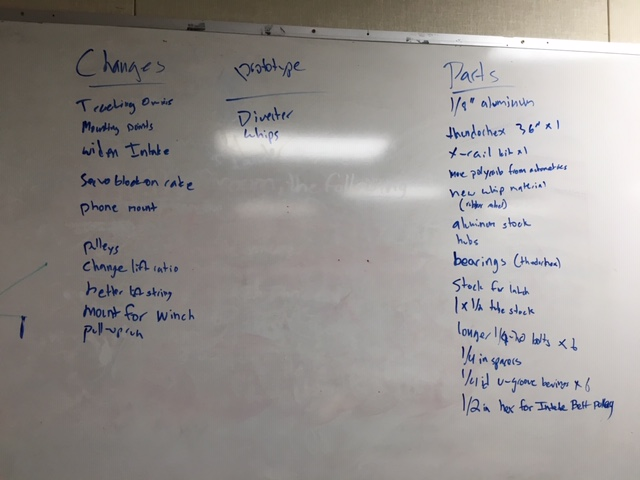
\includegraphics[width=.6 \textwidth]{14_12-03/images/IMG_0422.JPG}
    \caption{}
    \label{fig: Parts list}
\end{figure}
\subsection{H1: Diverter}

After the Burlingame tournament the team realized how complicated their approach to sorting and depositing the minerals in the lander were. This was because the system had too many steps and required too many different parts and space. After the tournament, various members of the team started hypothesizing of alternative solutions to sorting. One solution that was thought up was a single cartridge for the balls and cubes to go into where they would be read by color sensors to determine the arrangement of balls or cubes. When dumped in the lander a diverter would be used to push the balls or cubes in the one direction or the other to allow for easily scoring ten points. Ashlin and Aidan took on the task of prototyping this diverter. A problem they noticed is that the if the combination of minerals had both a ball and a cube then both items would roll out so fast that the diverter wouldn't be fast enough to sort the minerals. They fixed this problem by implementing a gate that would separate the two minerals and cause a delay between them so the diverter would have time to re-position. Aidan and Kelly tested this the diverter and found it worked fairly accurately.

\subsection{H2: Latching Hook}

After Ben and Shawn prototyped the servo and pin latch mechanism, the team realized that a simpler design would be easier to control and manufacture. Ben started CADing the part and Kelly suggested they use math to find how thick they should make the aluminum. So Kelly, Ben, and Aidan started discussing it, they used a combination of physics and trigonometry to determine the stress as shown in figure \ref{fig:math} . Then they used the stress analysis tool in Inventor to see where the most stress was and were the aluminum would, in theory, bend or break as shown in fig \ref{fig:stress}. They found that the red was only around 1.5 ksi, so they looked up the max ksi before elastic deformation and found that it was around 40 ksi. So the aluminum was perfectly fine.

|\subsection{H3: Drive-Train Update}

After a rush finish for the drive-train, due to the Burlingame tournament. The team felt it was necessary to simplify the drive-train to allow for more room and more precise mounting of other mechanism to the drive base. Currently on the robot their is a separate aluminum plate that holds the intake to the drive-train (Insert Image), which is structurally  weak and allows for a lot of excess vibrations when the intake is running. As a result it was re-CADed so that the added on part was cut out with the inside plate as a whole (Insert Image) this allows for more room between each drive half, along with being more structurally sound. Another very important change is the placement of the rear cross brace closest to the linear lift. It was moved closer to the motors to allow for more room, so that the lift motor and spool can be mounted directly under the lift for the pull down string (Before Image)(After Image). 

\begin{figure}
    \centering
    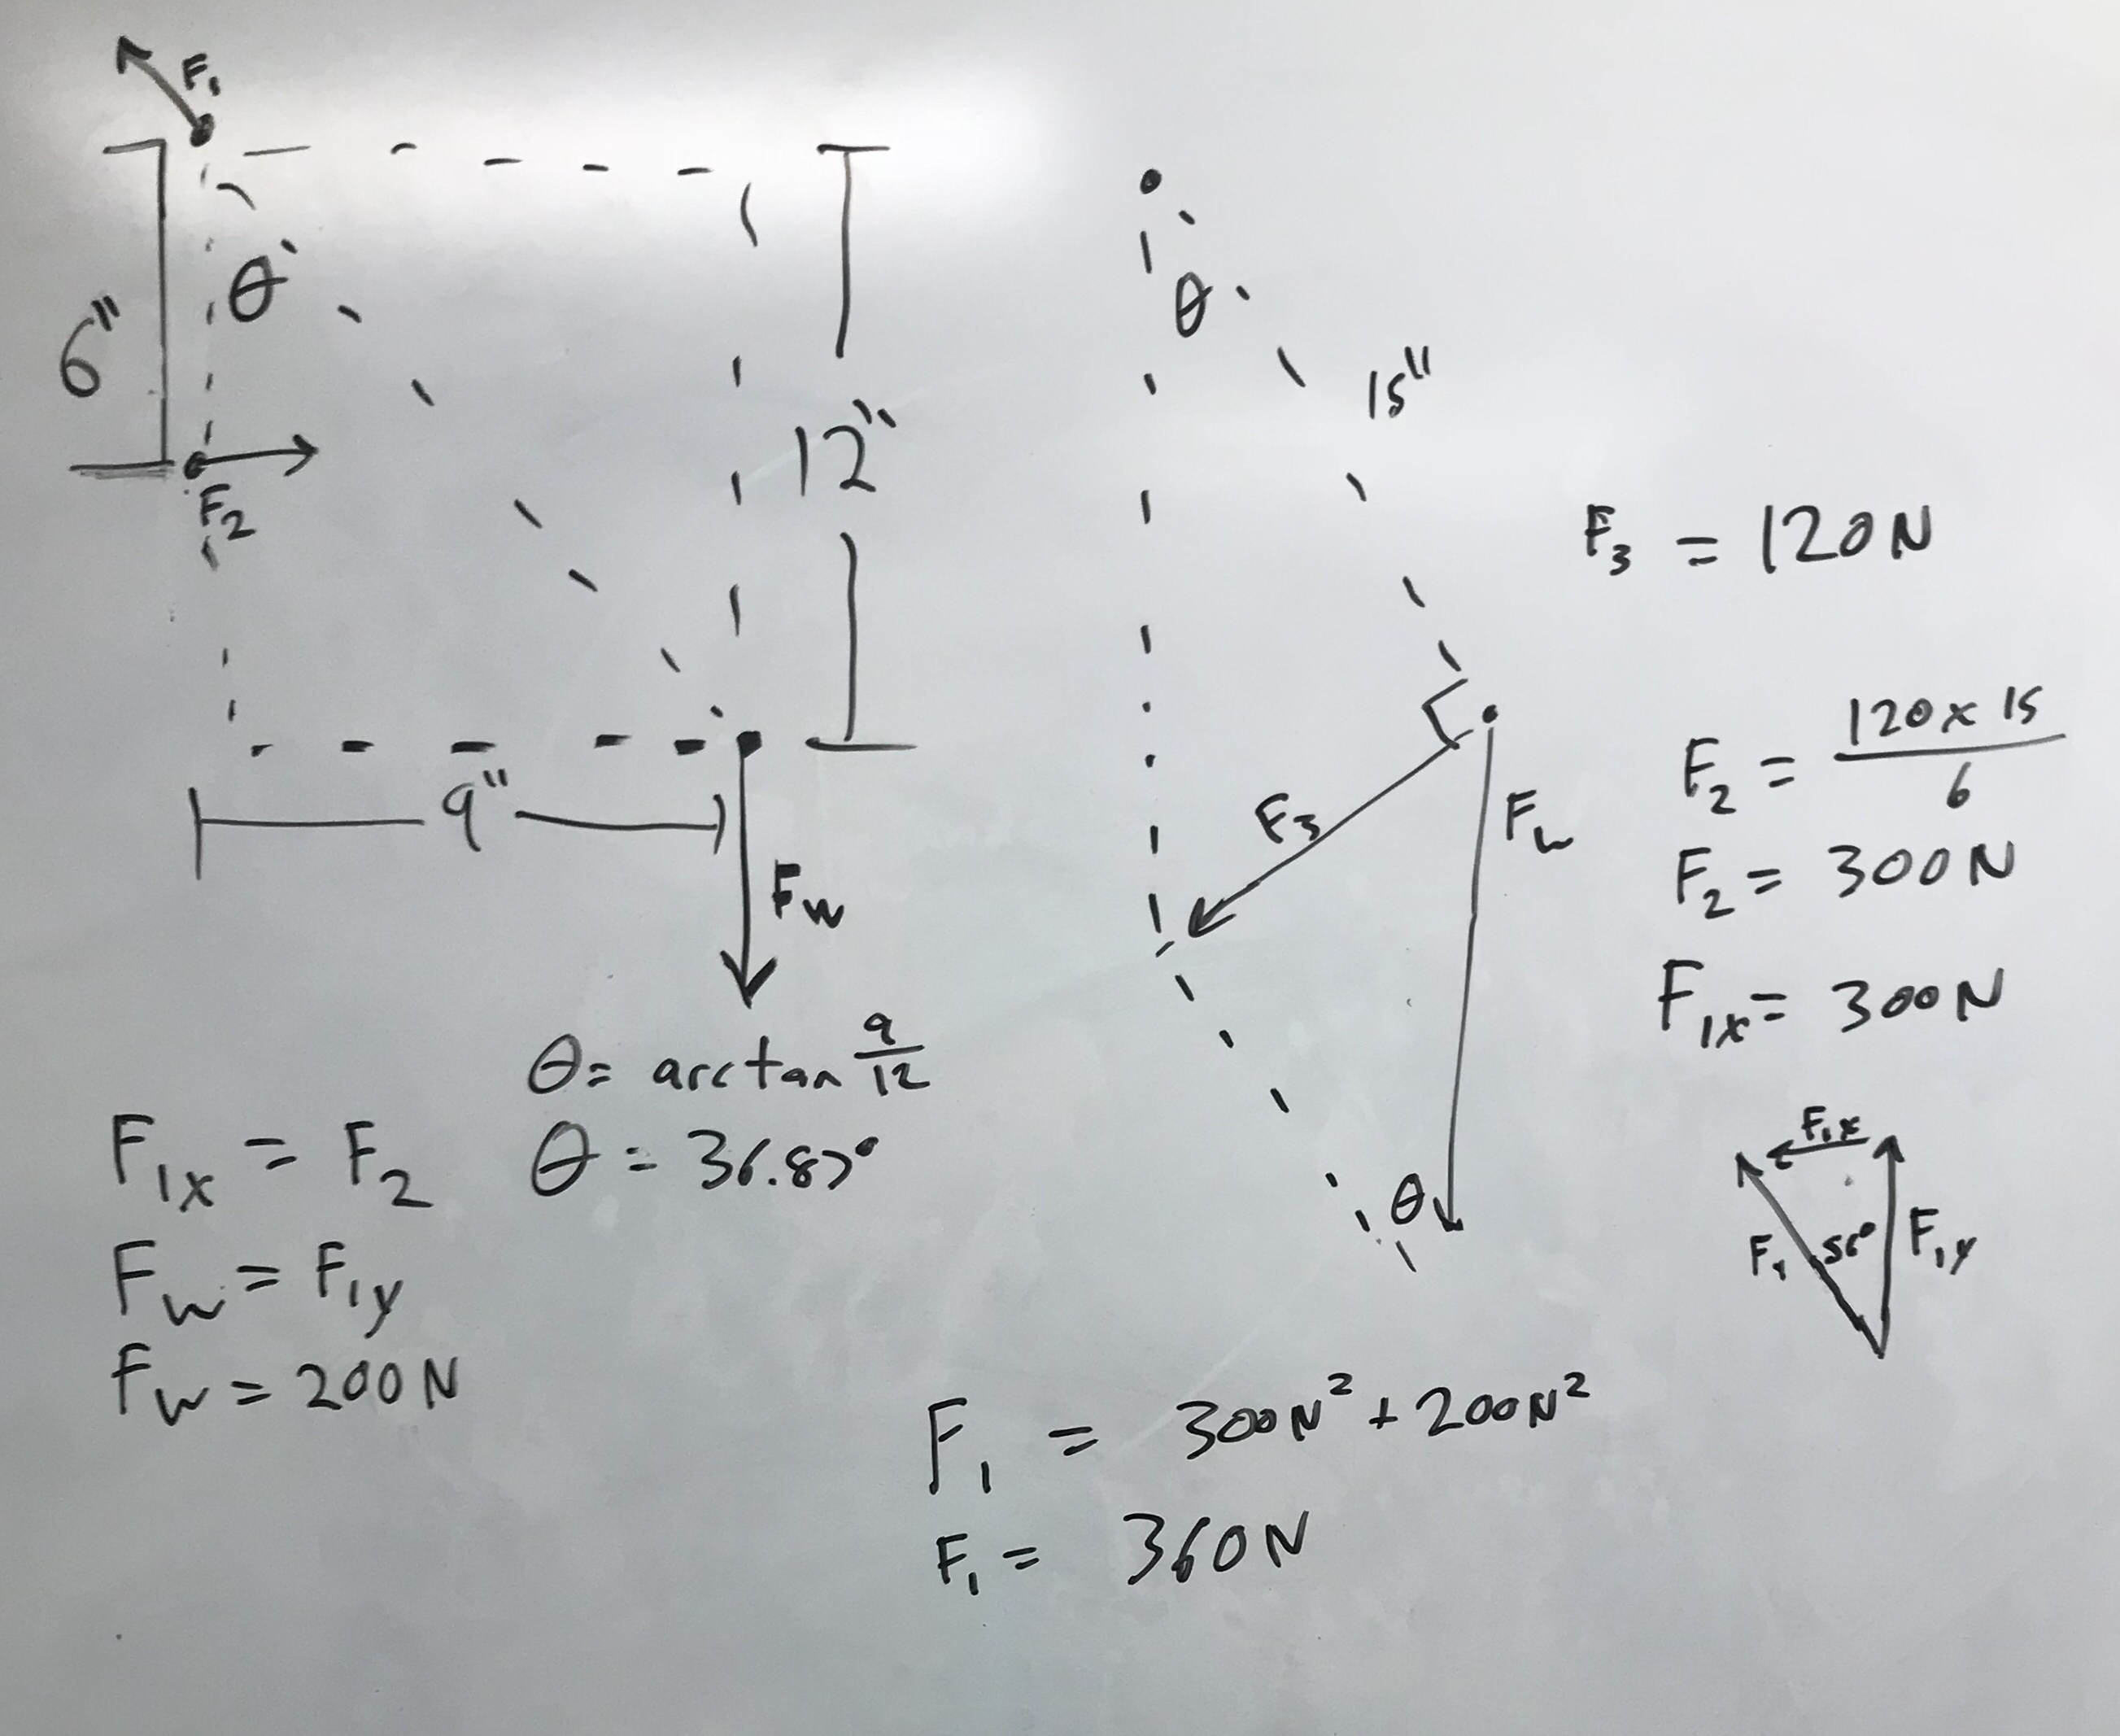
\includegraphics[width=.6 \textwidth]{14_12-03/images/Math.jpg}
    \caption{Stress Math}
    \label{fig:math}
\end{figure}

\begin{figure}
    \centering
    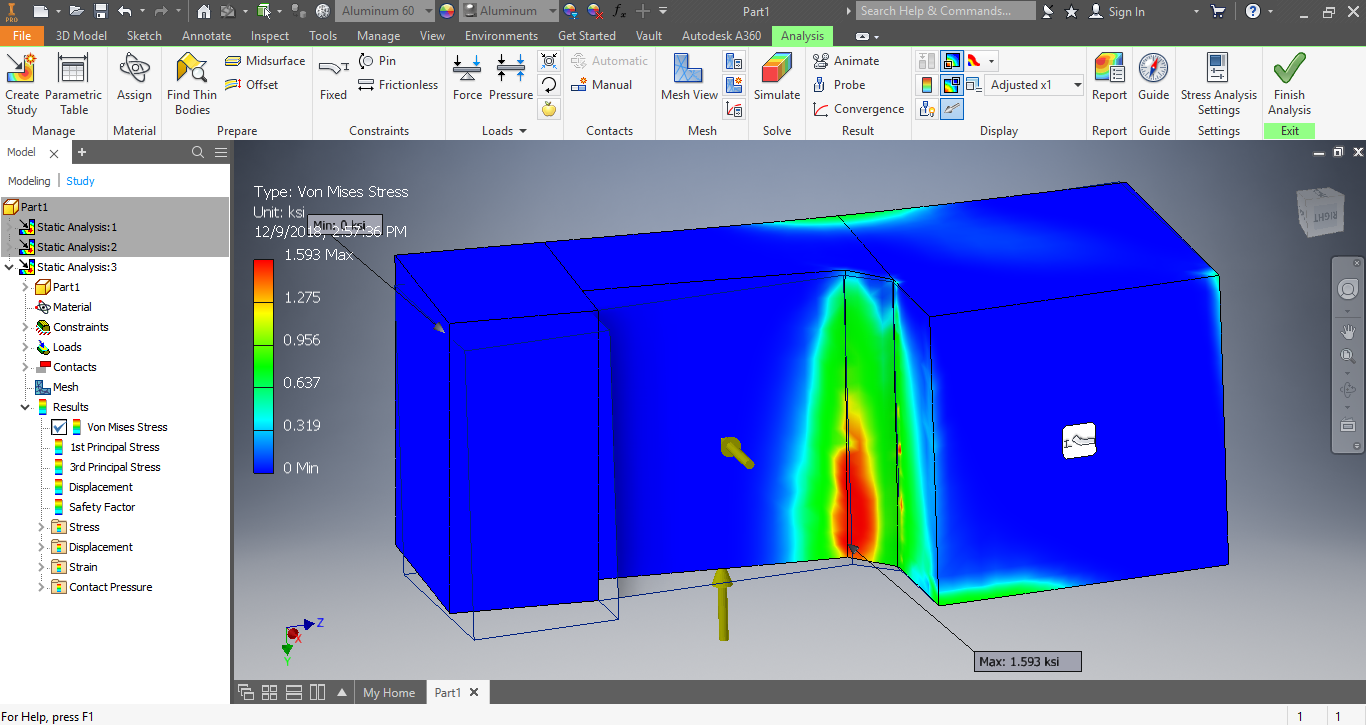
\includegraphics[width=.6\textwidth]{14_12-03/images/Stress_Analysis.png}
    \caption{Stress Analysis}
    \label{fig:stress}
\end{figure}
\subsection{H4: }
}\subsection{S1: Make a GET Request from Orange Alliance API}

When you need to obtain data from an API, you can use a GET request. In order to request something from an API you need to have an API key and use specific routing commands. Since Emma is going to use Java for this she made a Java application using the IDE Intellij. She had never done a GET request before, let alone in Java, so this was an interesting experience for her. \\

Emma used a website called Mkyong.com that provided an example of a GET request that would return the version of the API. Although Emma could have just control C and control V-ed this into her application but, it was important that she knew how this code operated so that she could understand it for the future. Therefore, Emma spent a long time learning what each line of code did and how it was vital to getting a request. Finally, after fixing a couple of mistakes, the code did what it was supposed to do (yay!) and Emma, through lots of Googling, was able to thoroughly understand how it works. \\



\clearpage \newpage \section{Week \thesection} 
\subsection{Hardware Goals}
\paragraph{H1: Diverter}
Creating a fully working diverter and mounting it to the robot
\paragraph{H2: Testing X-Rail Slides}
 Testing and assembling the X-Rail slides.
\subsection{Software Goals}
\paragraph{S1: Set up a console for the Prescouter}
 Make a usable console for the prescouter.
\newpage
\subsection{H1: Diverter}

After the success of the prototype diverter the team decided to make it their primary sorting and depositing system. Ashlin and Aidan began to make a hopefully final version out of poly carbonate. They used poly carbonate because they knew that when they were depositing minerals they were only going to be able to tip the diverter at a small angle and so they needed a slippery material so the cubes wouldn't become stuck. The completed diverter is show in figure  \ref{fig:diverter}.

\begin{figure}
    \centering
    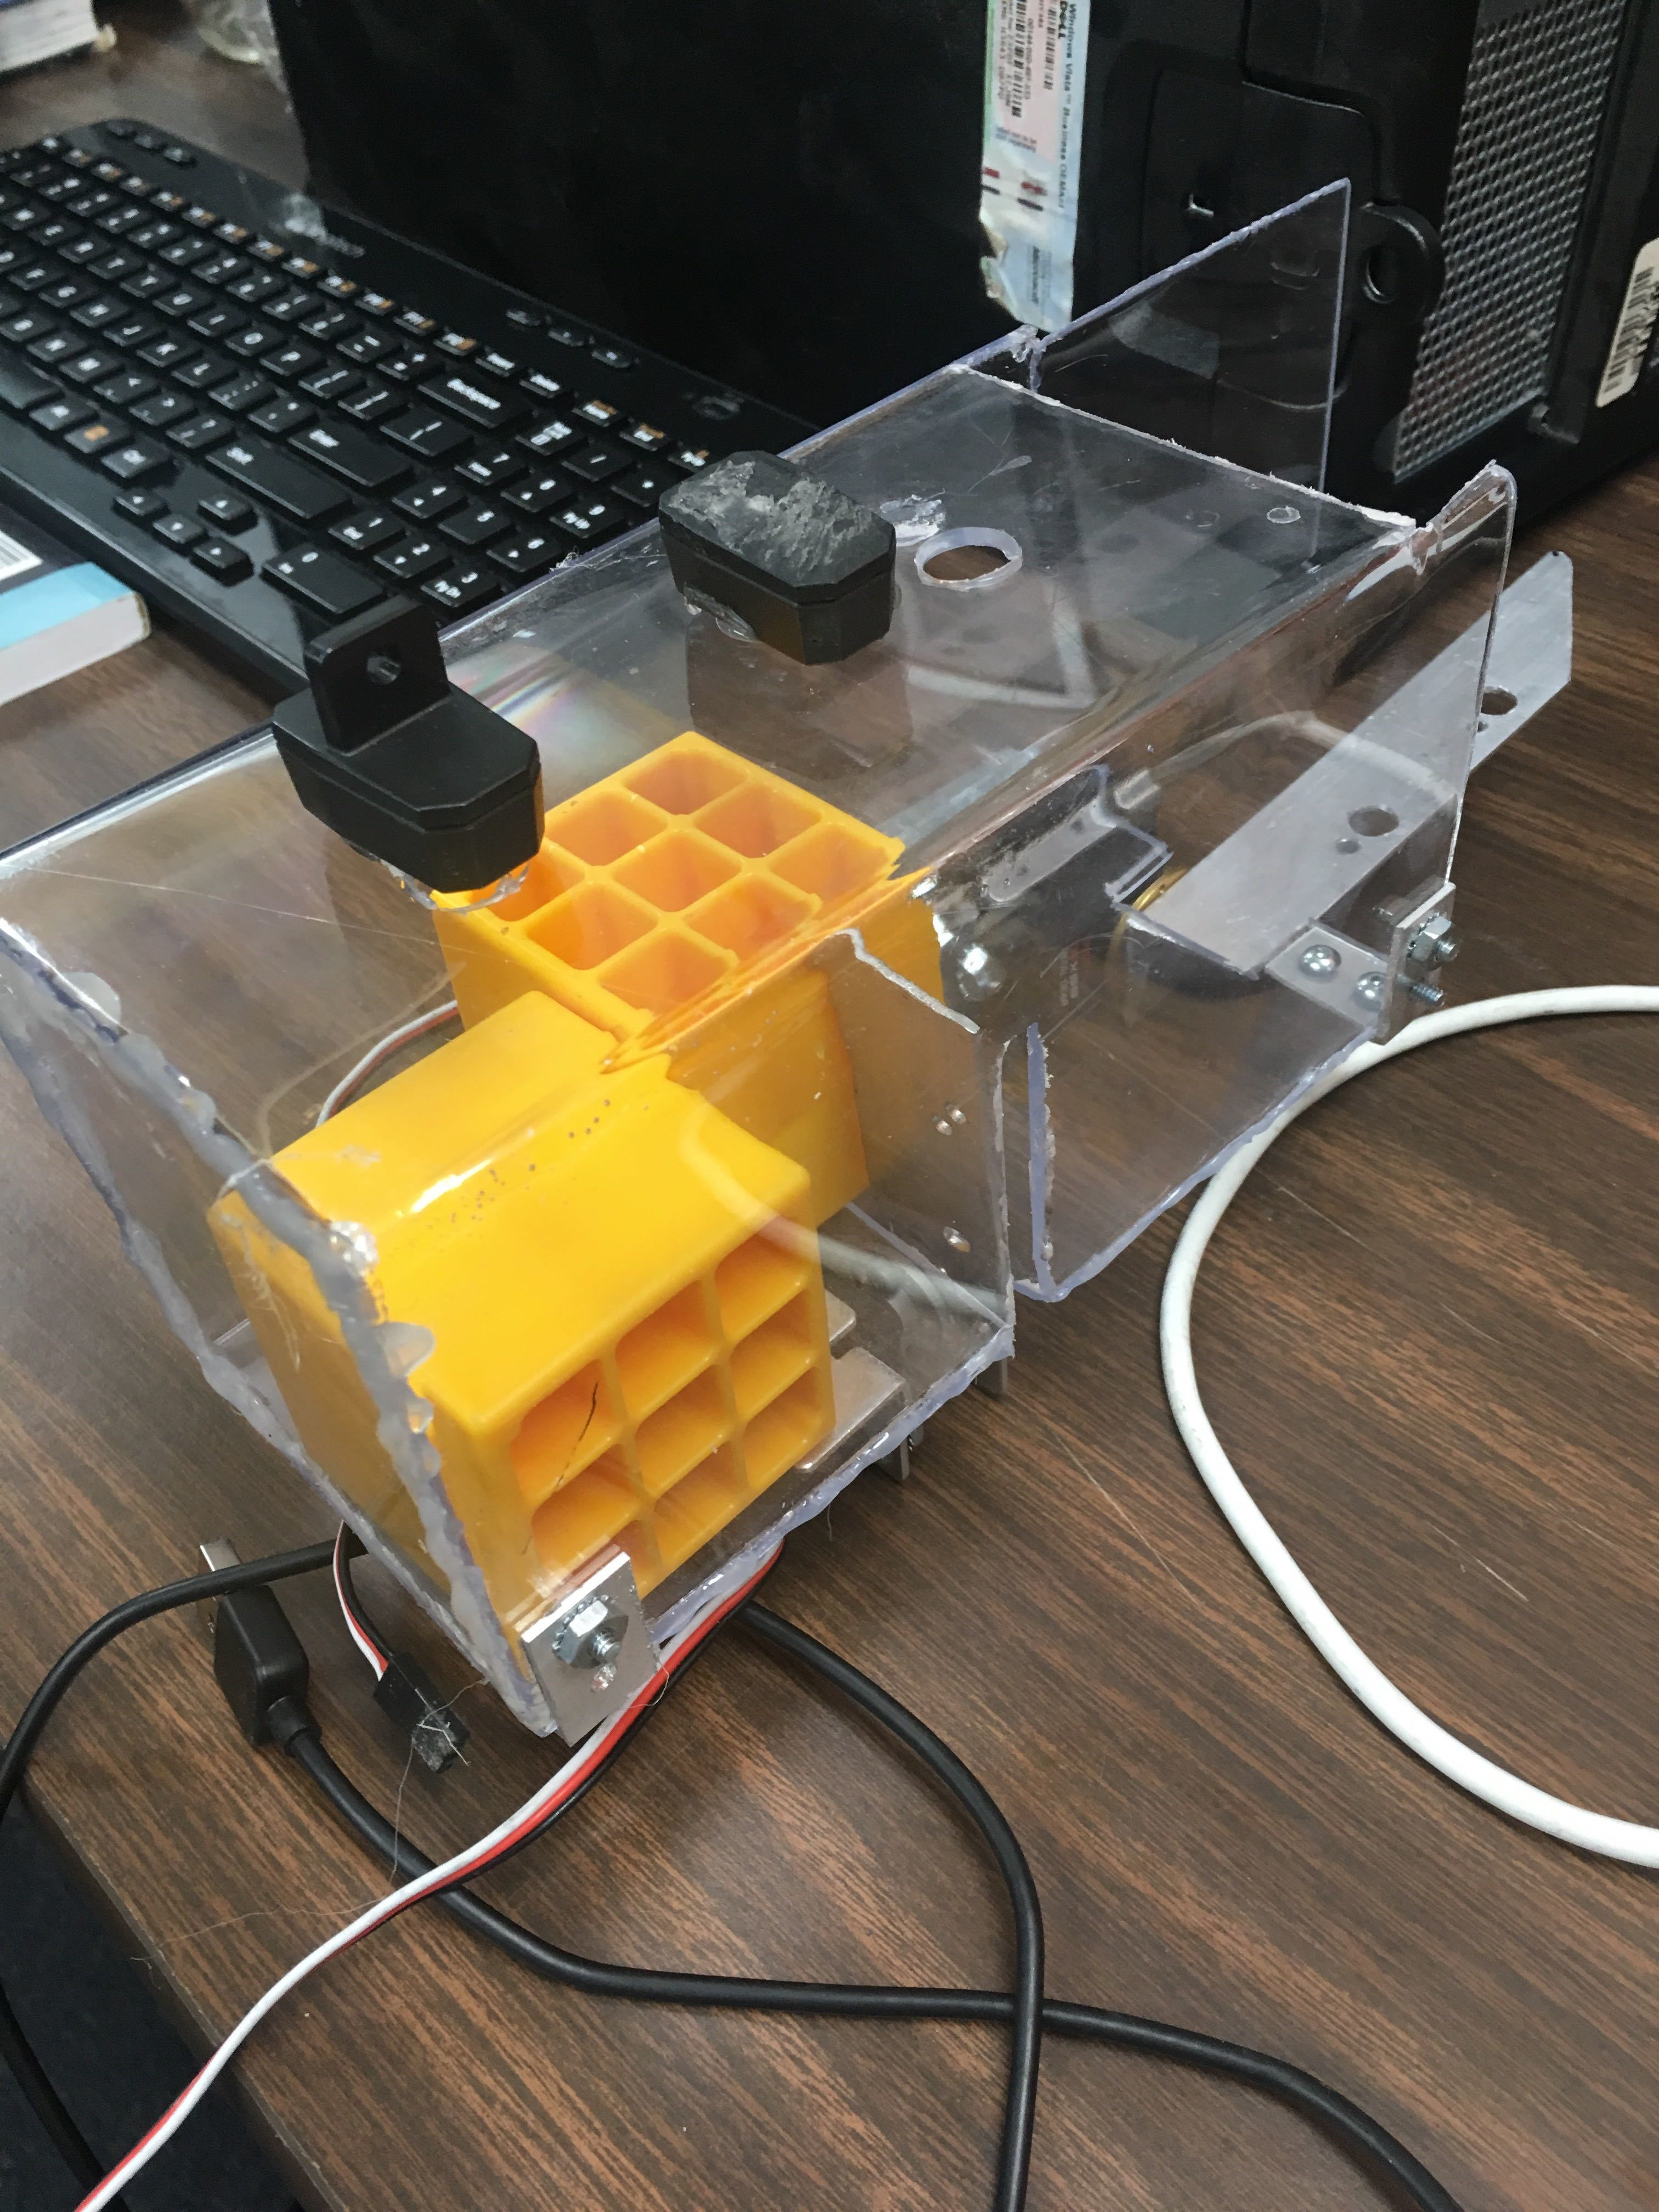
\includegraphics[width=.6 \textwidth]{15_12-10/images/Diverter.jpg}
    \caption{Diverter Design}
    \label{fig:diverter}
\end{figure}

\subsection{H2: Testing X-Rail Slides}

Now that the X-rail had arrived from order, the team saw fit to construct a set of X-rail for testing. Jon, Ben, and Shawn took on this task. Given that the X-rail was as yet unproven, it was important to run it through its paces to ensure it was a good option. While on paper the X-rail was perhaps the best option for the horizontal linear motion the team was looking for, in practice things could be different. After Jon, Ben, and Shawn completed the X-rail kit, Jon began testing the X-rail slide. He tested that the surgical tubing was taught enough to pull blocks and balls back to the intake, he tested how and where it would be mounted, he tested the rigging, and he tested where the servo for the rake would mount. After testing all these qualities, Jon determined that the X-rail would be a good replacement for the Rev Linear slides. While the X-rail would function in almost the same way as the Rev linear slides; A couple things would have to be changed. The rake servo would have to be mounted lower, and the rake would have to rotate from side to side rather than up and down. Being that the X-rail is larger than the Rev slides, the rake servo would need to be mounted lower so the rake could be as close to the ground as possible. Even with the servo being mounted lower, it was still high enough off the ground that the rake would have to deploy in a different way. The team decided that having the rake swing down from the X-rail would not only be a more efficient use of space, reduce wobble and strain, but would also more easily allow the use of X-rail. This would require the design of a new rake which set to work on. 



\subsection{S1: Set up a console for the Prescouter}

The next step for the prescouter was to make it usable. This was accomplished by using a console. Emma chose to make a simple console application first, rather than tackling a full UI because it is easier to work out all the kinks of the code before adding the additional stress of a making a functional UI. So for now, having a console will satisfy the needs of the app. Since there are different commands for the Orange Alliance API, Emma needed to make it so that what the user typed in would be the URL that was sent to the API. She accomplished this by using a scanner. This was the first time Emma used a scanner and at first she thought it would be rather difficult but it turned out to be fairly simple. 

Emma realized that it might be useful to keep the program running in a loop so that the user didn't have to play the project again and again. She used a while loop with a constant variable set to true, so that the program could run indefinitely. With this little addition done, the console was fully functional as seen in figure \ref{fig:console}. The next step for the prescouter is parsing the JSON response from the API so that it is easier to read. 

\begin{figure}
    \centering
    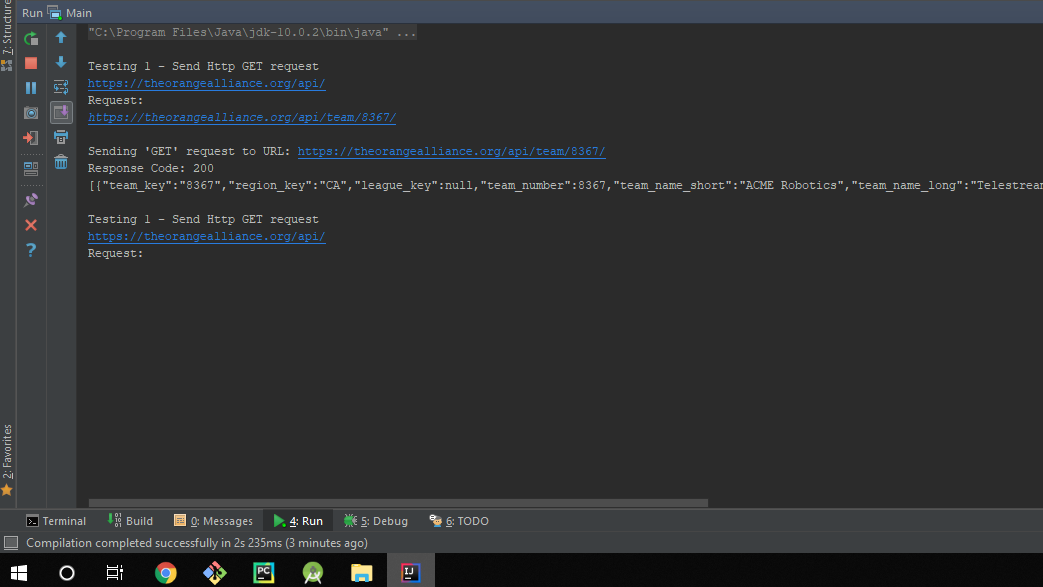
\includegraphics[width=.6 \textwidth]{15_12-10/images/console.png}
    \caption{The Console for the Prescouter}
    \label{fig:console}
\end{figure}
\clearpage \newpage \section{Week \thesection} 
\subsection{Hardware Goals}
\paragraph{H1: Intake Gate}
 Creating a servo powered gate at the back of the intake.
\paragraph{H2: Attaching the rake and testing the intake}
 Finding and testing a different way to attach the X-rail.
\paragraph{H3: Building the pulley system for the lift}
This week, Ben made the pulley system for the lift.
\paragraph{H4: Deconstructing Robot}
 Take apart parts of the robot in preparation for the coming weeks. 
\subsection{Software Goals}
\paragraph{S1: Tune lift kinematics}
Tune the control loops to run the lift automaticaly
\newpage
\subsection{H1: Intake Gate}

After completing the attachment of the diverter to the robot the entire intake was almost complete. Aidan realized that to meet the two materials maximum rule the intake was going to need another gate that would stop any more materials from going into the diverter. Previously the team had thought that this problem was already taken care of with the cartridge itself. The cartridge was supposed to be able to only hold two and then the gate at the top of the cartridge would close and stop any excess minerals. This was not going to work because the way that gate closed would actually pull in more minerals and get them caught in the robot. To fix this problem a gate needed to be created at the top of the intake. Shawn created this gate as shown in figure \ref{fig:gate}. This fixed the problem because it stopped any extra minerals from going into the diverter and the extra minerals could easily be repelled with the intake running reverse.

\begin{figure}
    \centering
    \includegraphics[height=6cm]{16_12-17/images/gate.jpg}
    \caption{Intake Gate}
    \label{fig:gate}
\end{figure}

\subsection{H2: Attaching the rake and testing the intake}

Now that all systems of the intake at least had one prototype, the team wanted to attach them all to the robot for testing. The team quickly ran into complications with the rake however. Originally, ACME planned to mount the rake in a similar fashion the the Rev linear slides by bolting the bottom to the outside drive plate. However, the X-rail was much taller and longer then the Rev slides; meaning the servo the rake mounted to would be to high off the ground and outside the 18'. The team first tried to mount the servo lower with a long bracket. This turned out to be too flimsy and was quickly scrapped. Next the team tried an elongated arm from the servo to the rake. This produced similar problems of stability and got in the way of deployment. The team then discovered that they could mount the X-rail upside down by mounting it from outside drive plate. This solved the issue of the servo being too high up and far out. It would also streamline the whole design and was stronger than any previous solutions. After some brainstorming about how exactly to mount it the team decided on cutting a new outside drive plate with an extended top that would curve over and mount to the top of the X-rail via bolts. (Fig 0.2). To test this idea, the team created a prototype and mounted it to the robot. This way they could test if it was feasible before cutting a new drive plate. Which would use valuable material and time. The tests were successful and the team is going ahead with the design. 

\begin{figure}
    \centering
    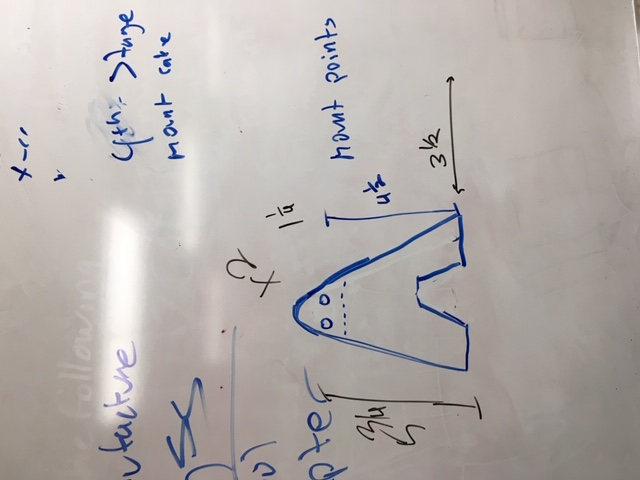
\includegraphics[height=6cm]{16_12-17/images/x-rail_mount.JPG}
    \caption{Sketch of X-rail mount on the outside drive plate}
    \label{fig:Mount Sketch}
\end{figure}

\begin{figure}
    \centering
    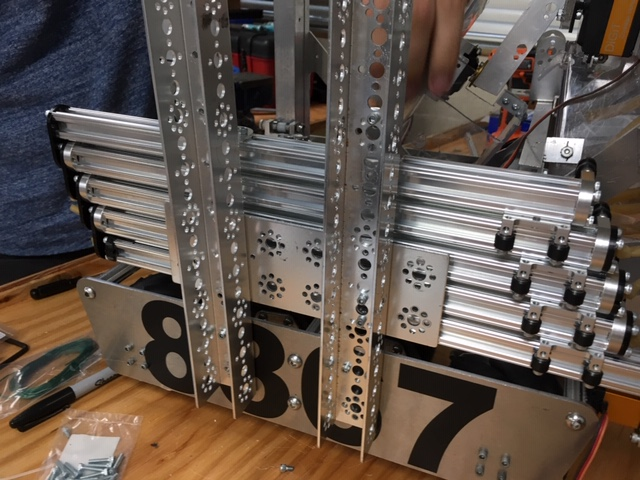
\includegraphics[height=6cm]{16_12-17/images/mount_proto.JPG}
    \caption{Prototype outside drive plate mount}
    \label{Prototype Mount}
\end{figure}

\subsection{H3: Building the pulley system for the lift}

This week Ben worked on developing the pulley system for the lift. He started thinking that he might use pulleys and tetrix L Brackets that already had holes so that he didn't have to cut new ones. Ben then cut down the side on on of them to try to get the bracket as close as possible to the side of the lift. He then used some v bearings to be able to string it. Then, after he adjusted the design, he made two more to put at the bottom and one to go at the top.

\subsection{H4: Deconstructing Robot}

After all the sub-systems had been tested Oren, Ben, Shawn, and Adian took apart the main portion of the robot, as to prepare for the coming week. They made sure to organize and keep all the necessary parts to make a smooth re-construction of version 2.0. There was a considerable amount of modifications made to fully built subsystems to make sure they would fit on the new drive-train. One of the changes that had to be made was to the intakes rollers length, due to the inner dimension of the aluminum plates increasing, which in turn increased the length of the rollers. 
\subsection{S1: Tune lift kinematics}

The lift needed to be motion profiled in order to run during auto (to get off of the lander, and then lower the lift back down), as well as to run it automaticaly during teleop, so the drivers only need to press a single button for the lift to automaticaly go to a set position. Because the two motors of the lift drive the same gearbox, it would not work to use the onboard PIDF velocity control. If the Rev Hub commanded different voltages to each motor, they could end up fighting each other, and potentialy burn out, or at least reduce the efficiency of the lift. To avoid this, Kelly decided to run the motors in an open loop mode, where the voltage applied to the motors will be commanded to the rev hub in a number between -1 and 1. This means that a feed forward constant will have to be used within the subsystem code, rather than onboard the rev hub. This constant relates the speed commanded, on the interval of -1 to 1, to the actual velocity of the lift, in inches per second. If this were the drivetrain, a opmode could run the lift to collect the neccecary data, but since running the lift too far in any direction could potentialy break the robot, Kelly did not feel comfortable running the lift autonomously until the control loop was tuned. Kelly instead ran the lift manualy, moving it up and down with the joystick at various velocities and positions, while logging the data. 

By preforming a regression on the data, Kelly determined $kF$ to be $0.0917$. Kelly also determined 14 m/s, 30 m/s/s, and 30 m/s/s/s to be reasonable values for $maxV$, $maxA$, and $maxJ$ respectively.

Kelly then tuned the lift PID loop. Because the lift only has one degree of freedom error is not the end of the world, and smooth motion is the priority, so Kelly omitted D from the loop, and kept P and I low. After the loop was tuned the lift was able to run to a desired position at the press of a button during teleop.

\begin {figure}
\centering
\begin{tikzpicture}
\begin{axis} [xlabel=Command, ylabel=Actual]
\addplot table [x=command, y=velocity, col sep=comma, only marks, blue, mark options={scale=.5}] {16_12-17/lift.csv};
\addplot +[no marks, red, thick, domain = -1:1 ] {x / .0917} ;
\end{axis}
\end{tikzpicture}
\caption {Actual vs. Commanded velocity}
\label {fig:graph}
\end{figure}
\clearpage \newpage \section{Week \thesection} 
\subsection{Hardware Goals}
\paragraph{H1: X-Rail Mounting}
 Mount the X-Rail.
\paragraph{H2: Cutting Drive plates}
Setting up and cutting inside drive-plates
\subsection{Software Goals}
\paragraph{S1: AHHHHHHH}
subsection {AHHHHHHH}
AHHHHH

\paragraph{S2: Characterize and tune the drive train}
 Empericaly determine the characteristics of the drivetrain, and use them to tune both the PIDF onboard velocity loop and the PID position loop for trajectory following during autonomous. 
\newpage
\subsection{H1: X-Rail Mounting}

This week the inner drive plates were cut. However, since the outer plates were not cut, the X-rail could not be mounted. As such, a stop-gap method was used to mount the X-Rail. While technically the X-rail was mounted before on Tetrix, it hardly worked. This meant that if the team wanted to have a functioning robot, they would need to create one that worked better. ACME wanted to meet a deadline for having the robot able functioning so it was important to make this stop-gap solution. Jon was assigned to create this. The easiest way to do this seemed to be by drilling mounting holes into two sheets of aluminum and folding them. It was important that the mounting solution be simple and quick to make because the deadline that the team needed to have a functioning robot by was fast approaching. 

\subsection{H2: Cutting Drive plates}

For the cutting processed we decided to use a CNC laguna, for its precision and accuracy rather than by hand or CNC plasma cutter.The job set up was pretty simple since we had been waked through it the previous time. The set up entailed us, to cut out two pockets two feet by 1 foot so as to allow our aluminum when screwed down, to rest flush with the top of the spoil board. We then orientated the board so that the bottom left corner of the board was at the X \& Y zeros, to allow for an easy tool path set up in Aspire. As an extra precaution in Aspire we added tabs to the material that would be completely cut out, so that the router wouldn't throw the loose aluminum pieces. Since this plate was CADed to have precise mounting holes, it required us to make two tool changes, not hard to do in the program, but required us to learn a new step, Tool Touch offs. When we had finished the program portion of the set up we moved back to the Laguna, were we started with setting our X,Y \& Z zero's. The Z zero had to be set to the bottom of the pocket because the Laguna cuts from the bed surface not from the material. Those zeros are very important to get as accurately as possible, because the tool switches and touch offs are based on the first bit and the said zeros. After we made sure everything was set up to the best of our ability, we began cutting, about half through the first pass on the profile the 1/4 O-flute bit snapped due to depth and side impact on the bit. We quickly switched the bit and reset all our zeros and tool touch offs, then resumed the cut. We later talked to a professional, who told us that the bit we were using was for 1/16th inch aluminum not 1/8th, so we ended up buying a new one to replace theirs.  
\subsection{S1: AHHHHHHH}

\subsection{S2: Characterize and tune the drive train}


Before the robot can be able to follow paths during auto, the control loops must be tuned. There are two cascading control loops that control the robot's position. The first is the PIDF velocity loop onbard the Rev Hub. Changes to the rev hub firmware this year mean that rather than commanding velocity in some unitless number between -1 and 1, velocity can actualy be commanded, in radians per second. This takes some of the complication out of the control system, because the constant that relates that unitless number to an actual velocity does not need to be found, but the onbard loop still has to be turned. 

The first step is to turn off the feedback components of the controller, by setting $kP$, $kI$, and $kD$ all to zero. To tune the feedforward constant, $kF$, Kelly first set it to 1. Then he wrote a opMode that gradualy ramped the commanded velocity up while the robot hurtled down a long strip of field tiles, sheporded by Emma. The opMode logged both the commanded velocity and the actual velocity reported by the Rev Hub. The velocities were recorded in radians per second rather than inches per second, because the velocity loop works with individual motors rather than the velocity of the robot its self. The measured data is shown in figure \ref{fig:graph}. While it is obvious that the real line of best fit should be of the form $y=ax+b$, that would not translate to a usable $kF$ for the velocity control loop, as the Rev Hub has no option to set a $kStatic$. Because of this, static friction will have to be ignored, and the regression calcualted in the form $y=ax$, which would make $kF = \frac{1}{a}$. This form of the regression still leaves the coeficient of determination sufficiently high, and even if there is some leftover error, the feedback portion of the loop will take care of that. After preforming the regression, $kF$ is found to be $12.579$. If the mass of the robot significantly changes, this process will have to be preformed again to find the new coeficients.

The next step in the tuning process is to determine the feedback components of the velocity control loop, but this is made easier by a reasonably tuned feedforward component. It is important to tune the feedback coeficients, because the default tunings are meant for an unloaded motor. The motors respond well then just a bare shaft is spinning, but the coeficients are much too low once they are moving around the mass of a 18kg robot. First $kP$ is tuned, by increasing it until the loop becomes unstable, and then backing off a bit. Then $kD$ is added to dampen the rest of the oscilations, and $kI$ to take up any remaining constand error. To tune these coeficients the robot follows a series of motion profiles to travel in a square in the middle of the field while Kelly watches on the dashboard, adjusting the coeficients as needed. Because changing the coefficients on the Rev Hubs requires stoping the motors and re-seting their run mode, the coeficients can only be updated between paths.

After finding a reasonable tuning for the velocity, Kelly tuned the positional PID. The same process was repated, driving the robot in a square around the middle of the field, but this time the positional coeficients were tuned. The corrections determined by the three positional PID loops, axial, lateral, and heading, are added to the velocity calculated from the trajectory to determine the velocity commaned to the drivetrain, which is turned into the velocity commanded to each motor. Because the velocity loops reduced the error quite a bit to begin with, only P terms were needed on the positional loops. 

With the control loops tuned, the robot was now ready to begin executing paths.

\begin {figure}
\centering
\begin{tikzpicture}
\begin{axis} [xlabel=Command, ylabel=Actual]
\addplot table [x=target, y=actual, col sep=comma, mark=none, blue] {17_12-24/fftuner.csv};
\addplot +[no marks, red, thin, domain = 0:420 ] {x / 13} ;
\end{axis}
\end{tikzpicture}
\caption {Actual vs. Commanded velocity, with line of best fit}
\label {fig:graph}
\end{figure}
\clearpage \newpage \section{Week \thesection} 
\subsection{Business Goals}
\paragraph{B1: Writing Tournament Presentation}
 Present at the county writing tournament.
\subsection{Hardware Goals}
\paragraph{H1: X-rail mounting work around}
 Figure out a way to mount the X-rail.
\paragraph{H2: Re-Constructing Robot}
 Re-constructing Robot version 2.0.
\subsection{Software Goals}
\paragraph{S1: Parse the JSON Response}
 Use a JSONArray to parse the JSON response from the API
\newpage
\subsection{B1: Writing Tournament Presentation}

The writing tournament is an event in Nevada county for 6th and 7th graders. There are three parts to the tournament, the response to a presentation, the creative writing piece, and letter writing. They always have quest speakers and this year, ACME was asked to come. \\

Emma and Kelly prepared a half an hour presentation about ACME, FIRST, and  their 2017-18 season. The presentation basically told the story of their journey to Worlds with important information like how their design process and how software works mixed in. The students participating in the event were given a prompt to respond to. The prompt this year was "What makes a robotics team successful?" ACME made sure to include multiple ways for this question to be answered. For example, a robotics team can be successful by being Gracious Professionals, but also by doing well during competition. \\

The presentation went off without a hitch and the kids seemed to enjoy it as well. The participants were given a chance to ask Kelly and Emma questions after they were done with the presentation, and had several in depth questions that needed answering. After that, the students wrote their essays, which were later graded by a group of teacher judges. ACME got a chance to read the essays and include some of the winning ones in \textbf{Appendix D of the Business Notebook}. \\

This presentation was a great way to connect with more students in the community, especially those that enjoy writing and could be potential recruits to facilitate the engineering and business notebooks in the future. \\


\subsection{H1: X-rail mounting work around}

With the new outside plates now cut, the team could begin the final stages of fabricating the robot. There was a problem however, the part that was supposed to be bent over to mount the X-rail from the outside drive plate had broken off during the bending process. This caused the team to learn the hard way that aluminum is not suited for 90 degree bends. To overcome this problem, Jon bolted two Tetrix brackets to the inside of the outside drive plate. This acted almost exactly as the originally mounts would have. Jon did it this way because it was quick, simple, and functional. With a "robot done" deadline fast approaching, this was likely the best solution. While this was neither an elegant or permanent solution, it was at least functional.

\subsection{H2: Re-Constructing Robot}

After the majority of the newly fabricated parts were completed, we began building version 2.0. The build process the second time around was much faster and went very smooth. We completed the reconstruction with in two meetings, and then began the long and tedious process of wiring everything up. As a team we have learned from past experience that wiring and organization is very important for a functional robot. Organization allows for easy fixes when necessary and creates no confusion when working through software and hardware issues, this is an area that in the past has been neglected. But we have dedicated time and effort to make sure that wiring is cosmetically pleasing and concise. 
\subsection{S1: Parse the JSON Response}

With the prescouter, the response from the API is in JSON, which is very difficult to read as it is all strung together. Since this app is specifically made to make prescouting easier, it was important to parse the information. As Emma had no experience parsing before, she spent some time researching the basics before attempting to write the code. She decided to use a JSONArray to parse the data since the response was an array. This array consists of the JSON response from the GET. Then, Emma made JSONObjects for each key then used the array to get the value. Finally she printed the result to the console. Here is the JSONArray that she used to parse the data. 

\begin{lstlisting}[language=Java]
String jsonResponse = response.toString();
JSONArray array = new JSONArray(jsonResponse);
JSONObject teamKey = (JSONObject) array.get(0);
System.out.println("Team Key: " + teamKey.get("team_key"));

\end{lstlisting}

Each key in the array has a separate JSONObject in order to parse it. As this is a lot of code to have in the Main class of her application, next Emma has decided to make each command she will use into a different class and then call it in Main when she needs that specific data parsed. 
\clearpage \newpage \section{Week \thesection} 
\subsection{Hardware Goals}
\paragraph{H1: Lift Cross brace and LED side plates}
 Discussing an alternative cross brace and decorative side plates.
\paragraph{H2: Adjusting the angle of the diverter cartridge}
 The diverter cartridge angle needs to be changed to allow for cubes to fall out.
\subsection{Software Goals}
\paragraph{S1: Introduce OOP to the Prescouter}
 Use Object-Oriented Programming procedures to simplify the PreScouter.
\newpage
\subsection{H1: Lift Cross brace and LED side plates}

Most of the lift had been completed and one of the only things left was to create the cross brace at the top of the lift. The cross brace was necessary because without it the entire lift would wobble five to ten degrees when at max height. While Aidan created the brackets on the side of the lift to hold the cross brace, Aidan, Kelly and Oren discussed what they wanted to make the cross brace to be made out of. They decided that instead of just the metal plate running across they wanted to make the cross brace out of cast acrylic so that they could engrave patterns into the acrylic and light it up with LED's.They decided to do this with the acrylic instead of poly-carbonate because the poly-carbonate would melt a little when engraved. They then realized that they could also create similar illuminated plates on the side of the robot. However before these plates could be cut the designs needed to be created. Since this might take a few days, Aidan created a temporary cross brace that would serve until then.

\subsection{H2: Adjusting the angle of the diverter cartridge}

When most of the intake had been completed, Kelly, Aidan and Oren decided to fully test the diverter and lift. One thing they realized is that if there was a cube in the back of the diverter, the cube would not gain enough speed to roll out. They decided that the angle of the diverter needed to be increased to allow for this. Aidan fixed this problem by slightly cutting into the arm from the diverter to the servo which allowed the diverter to tilt farther as shown in figure \ref{fig:Cutout}. Aidan tested this and the cube gained sufficient speed with the new angle.

\begin{figure}
    \centering
    \includegraphics[height=6cm]{19_01-07/images/DiverterAngleCut.jpg}
    \caption{The cut to increase diverter angle}
    \label{fig:Cutout}
\end{figure}
\subsection{S1: Introduce OOP to the Prescouter}

In order to simplify the code in her Main class, Emma decided to use Object-Oriented Programming methods to call the different commands she intends to use while prescouting. She knew what object-oriented programming was, but decided to refresh her memory via the internet to make absolutely certain she understood the concept. \\

After doing that, Emma picked out which commands from the API she wanted to use. She decided that she wanted to be able to get information about the team, their match performance, the awards they had won, the results of their tournaments, and the events that they attended. Emma thought that these commands would yield the most information about the team she would be prescouting. She made a class for each command at set to work. Emma used the exact same method to parsing the JSON response in each class and also set it up so that they could be easily called in the Main. After a lot of tweaking, Emma got it working. It is now very easy to call commands in Main and her code is a lot cleaner. It is very clear as to why OOP is very useful and an important tool to use while programming. 
\clearpage \newpage \section{Week \thesection} 
\subsection{Hardware Goals}
\paragraph{H1: New Team Marker placement}
 Find a place to mount the team marker.
\paragraph{H2: Wiring and Rev Hubs}
 Attaching the Rev Hubs, Battery, phone and wiring the robot.
\subsection{Software Goals}
\paragraph{S1: Deploy during auto}
 Use a proximity sensor and hall effect sensor to deploy during auto
\newpage
\subsection{H1: New Team Marker placement}

After some testing, it was determined that the current placement for the team marker was unreliable. The team marker had previously been placed high on the rear of the robot which caused a great deal of deviation in where the marker landed. Ashlin and Jon were set to this task. They figured that since the problem was that the marker was too high, they would simply put it lower on the robot. This proved to be a little tricky as there was not much space on the lower portion of the robot. The entire right side was taken up by the X-Rail and the left side had both rev hubs on it. The only place that there was space was behind the rev hubs and in front of the lift. Now that they had a place to put it, Ashlin and Jon had to figure out how it would deploy. The original method of deployment (a vertical arm the marker would fall off of when it was swung down) would not work here as there was not enough space. They then came up with the idea of a kicker that push the marker off the side of the robot. They liked this idea because it allowed the servo to sit above the marker, saving space, and it would be more reliable than the previous method. The only problem with this method was that there was nothing stopping the marker from simply falling off the robot. To remediate this problem, Ashlin cut a V shaped fork into the arm that pushed the marker off. The fork could then slide over a section of the marker, holding it in place. This solved the problem, and after some testing the new deployment method worked reliably. 

\subsection{H2: Wiring and Rev Hubs}

After most of the subsystems were built the team could then find permanent positions for the rev hubs, battery and phone mount. The team decided to put the rev hubs over the left side wheels because that is where there was the most room and the lowest chance of them getting damaged. To do this Shawn created a poly carbonate sheet that attached to the aluminum side plates and served as a firm attachment place for the rev hubs. Oren then realized that the danger with the rev hubs being there is the chance that wires could get caught in the drive train. To prevent this he created an aluminum plate to attach over the left side drive train to prevent important wires from falling in. Once the rev hubs were mounted the next important thing was to wire all the servos, motors and sensors. The difficult part of this was how to get the wires from the diverter servos because the diverter moved around so much. Kelly fixed this problem by using a wire track that could hold the wires safely inside while matching the up and down motion of the lift. The wires still needed to be run to the other side of the robot and the intake shield attachment bar served as an ideal wire trail from the right side to the left. Once all the wiring was complete the battery and power button were mounted in easily accessible locations and a temporary phone mount was created.


\subsection{S1: Deploy during auto}

Kelly worked on deploying from the lander during auto. Because the exact position at at which the robot is initialized may vary, using the encoders would be an inconsistent way to deploy. To consistently determine the robot's distance from the ground, Kelly decided to use a IR proximity sensor mounted at the bottom of the robot. After mounting the sensor and verifying that the robot's full range of travel would be encompased by the sensor's usable range, Kelly took the sensor off to linearize. Because it is an ir sensor, it measures distance by the intensity of reflected IR light. This means that there is a nonlinear relationship between the voltage returned by the sensor and the distance between the sensor and the ground. Before a loop can sucessfuly be closed around this sensor, the reading must be linearized. Attempting to use a PID loop with a non-linear sensor yeilds different responses at different locations within the sensor's range. and can lead to either instability or inaccuracy. To determine this relationship Kelly and Aidan built a test rig that contained both the IR sensor and a linear potentiometer. The linear potentiometer would return a voltage porportional to the displacement of the stylus along its length. By logging the voltage returned by both the sensors, and offsetting the voltage returned by the potentiometer so that 0 corresponded to the IR sensor being in contact with the ground, Kelly found the relationship between voltage and distance. This distance is still unitless, but the important part is that it is linear.

After removing the unusable data at either end and preforming a regression, Kelly found the relationship to be $d=0.3928 v^{-1.66868}$. 

Kelly then used this sensor to close a PID loop, consistently lowering the robot to the ground each time.


\begin {figure}
\centering
\begin{tikzpicture}
\begin{axis} [xlabel=Potentiometer voltage, ylabel=IR Sensor voltage]
\addplot table [y=dist, x=pot, col sep=comma, only marks, blue, mark options={scale=.5}] {20_01-14/linearization.csv};

\end{axis}
\end{tikzpicture}
\caption {Distance reported by sensor vs actual distance}
\label {fig:graph}
\end{figure}
\clearpage \newpage \section{Week \thesection} 
\subsection{Business Goals}
\paragraph{B1: Re-Organize the Outreach Section}
 Better organize the outreach section of the Business Notebook. 
\subsection{Hardware Goals}
\paragraph{H1: Cartridge Servo}
 Decreasing the load on the cartridge servo.
\paragraph{H2: Lift Skids}
 Brainstorm ideas for the lift skids.
\newpage
\subsection{B1: Re-Organize the Outreach Section}

ACME does a lot of outreach and the outreach section of the BN was looking a little bit disorganized. So, Kelly, Emma and Stephanie talked about how it could be better. They decided they needed clearer categories of outreach and came up with the following sections: 

\begin{itemize}
    \item Community Events
    \item FIRST Connections
    \item Team Building
\end{itemize}

They also realized that it would be good to explain what types of outreach events fell under each category. Also, instead of listing a bunch of future events they were planning at the end of the outreach section, those events could be split up by category and put under the explanations. \\

Emma took on the job of reorganizing. While in the process, she realized that Team Building needed to be split into two different section in order for it to make more sense. Before doing this, this section encompassed all of the events that helped build up the program in the county as well as events that the team does for fun. Thus, Emma created another section called Program Building, which housed all of the events that helped create a sustainable program in the community. Emma also added a ''Contents" section to the front page describing each category. She thought that it would be good to list what was in the category so that the judges could find things that seemed interesting to them. She made sure to order the Contents in the exact same order in which the individual events were listed for added easy accessibility. \\

When finished, the outreach section was much more organized than it was before. It was easy to find things and the categories made sense for the events that were in them. 
\subsection{H1: Cartridge Servo}

While Aidan and Kelly were testing the subsystems they saw that the cartridge servo was having trouble doing its full rotation. The servo especially had a problem when there was two cubes in the diverter because that is when it was carrying the most weight. The servo seemed to have trouble with the up part of its dump rotation as well as the up part of its reverse rotation. This caused a problem because it meant that whatever was used to help the servo needed to help it in both directions. Kelly and Aidan solved this by attaching a quadrupled up piece of surgical tubing to a stationary piece of the carriage and the other side to the servo horn. They connected it so that when the carriage was at its balancing point the surgical tubing had the least amount of tension. They did this so that when rotated farther clockwise then its balancing point the surgical tubing would help the servo in its reverse rotation and when rotated farther counterclockwise then its balancing point the tubing would help in the dump rotation. This helped the servo and allowed it to rotate in both directions with little difficulty.

\subsection{H2: Lift Skids}

With the lift now in working order, the team conducted some tests with it to see if it was up to snuff. The team quickly found that the lift didn't quite have the robot hanging the full four inches off the floor. The team put Aidan, Ashlin, and Jon on the job to fix this issue. They found that the robot was angled in such a way that the front was lower than the back. This meant that even though the back of the robot was four inches off the ground, the front was not. This was because the top of the lift stuck out farther (because of the hook) than the bottom. The trio thought they could add a plate to the back of the robot to alleviate this problem. They thought if they put a plate that stuck out as far as the hook, the robot would be flush with the lander along the entire robot. This would also make sure none of the lift or back of the robot would get caught on the lander and would just overall smooth the lifting and lowering process. They realized however that there was no where to put the plate that would interfere with the lift. All the available attachment points either moved with the lift or were too close to the 18 inch limit. This is when the team got the idea for skids. These would essentially act as skis for the robot to slide up the lander with. These were also smaller and less obtrusive than the plate. They decided to construct them out of poly-carb because of their flexibility (meaning it would be hard to break them) and because they would be easier to shape.
\clearpage \newpage \section{Week \thesection} 
\subsection{Software Goals}
\paragraph{S1: Finish the console version of the PreScouter}
 Finish how the PreScouter will be used in the console.
\paragraph{S2: Design double sampling paths}
subsection {Design double sampling paths}
%Design paths that sample both sets of minerals for extra points in autonomous

While supporting ARES at one of their qualifiers, Kelly saw that many teams either had no auto, or had an auto that only deployed from the lander. Kelly decided that this would make a auto that could disturb both of the gold minerals would be really good to have. In the scenario where an alliance partner did not leave the lander during auto, the location they started at would not matter, so these paths would only have to be designed for ACME's prefered start location, next to the crater. After experimenting by pushing the robot around, Kelly found that there was not enough room between the parked robot and the sampling field to approach the sampling field from the lander side, so the robot would have to first enter the depot, and then push the gold mineral toward the parked robot. This also happened to be an easier modification to make, because it only required duplicating the depot waypoint where the robot dropped off its marker, and adding a waypoint between them to disturb the gold mineral. Kelly tested the paths and found that they worked!

\begin{figure}
    \centering
    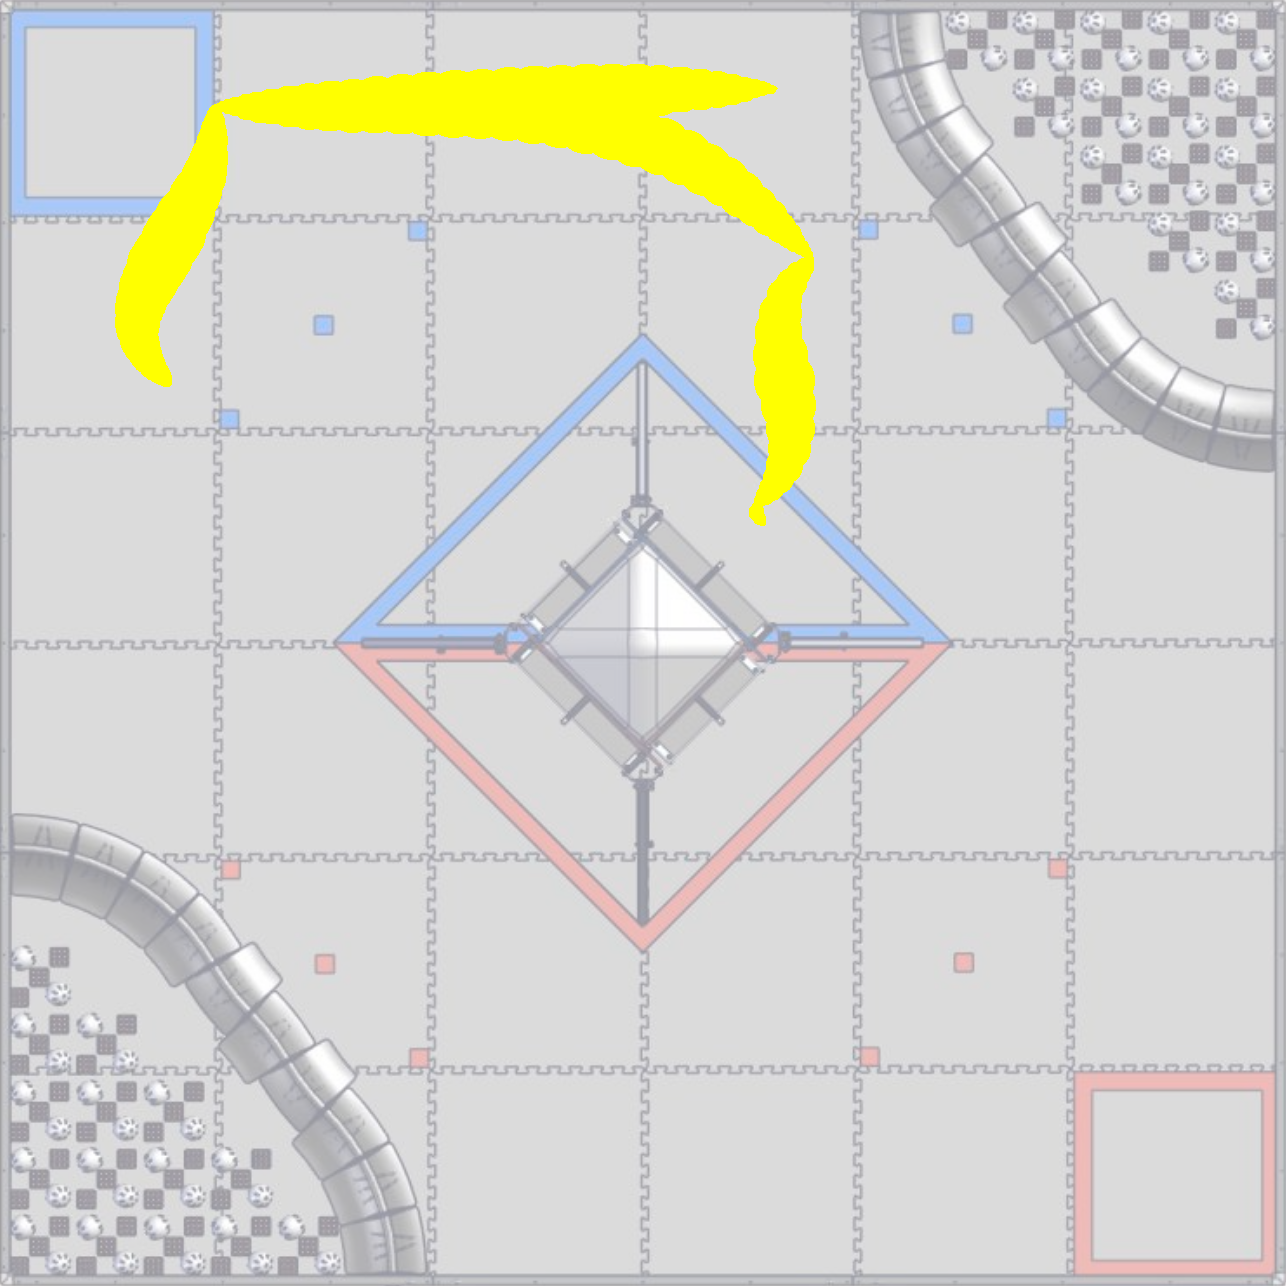
\includegraphics[width=.6\textwidth]{22_01-28/double.png}
    \caption{Double sampling path (line thickness corresponds to robot velocity)}
    \label{fig:double}
\end{figure}
\newpage
\subsection{S1: Finish the console version of the PreScouter}

This week, Emma finished the console version of the PreScouter. After calling each request class in Main and making sure that they were all working, Emma set about writing the code that would allow the user to make specific requests with ease. She decided to use a series of if else statements to accomplish this. First, the console asks the user what specific request they would like to make. There are only five requests a user can make because that is the only data that they need from the API. After making a request, Emma uses an if else function to prompt the user for the rest of the information needed in order to complete the URL to send to the API. Then, with the information from the user, Emma pieces together the URL and makes the GET request.\\

At the end of the sendGet() method, Emma used another if else function to print out the data. She decided to use another if else statement because it was easy to use the request from the beginning of the program in order to call the specific class that parsed the data. After she got that all working, the console version of the PreScouter was complete. \\


\subsection{S2: Design double sampling paths}

\clearpage \newpage \section{Week \thesection} 
\subsection{Hardware Goals}
\paragraph{H1: Drive Practice}
 Run matches with the drive team. 
\newpage
\subsection{H1: Drive Practice}

Over the week, the drive team ran practice matches to practice their driving skills. The drive team consists of Shawn and Aidan as the drivers and Emma as the drive coach. At the beginning of the week, they just ran the teleop part of a match, using a real FTC timer that they found on YouTube. They kept track of their scores and performance on the whiteboard, as seen in fig \ref{fig:chart}. For their first round of drive practice, they were averaging about 120 points during just teleop. 

\begin{figure}
    \centering
    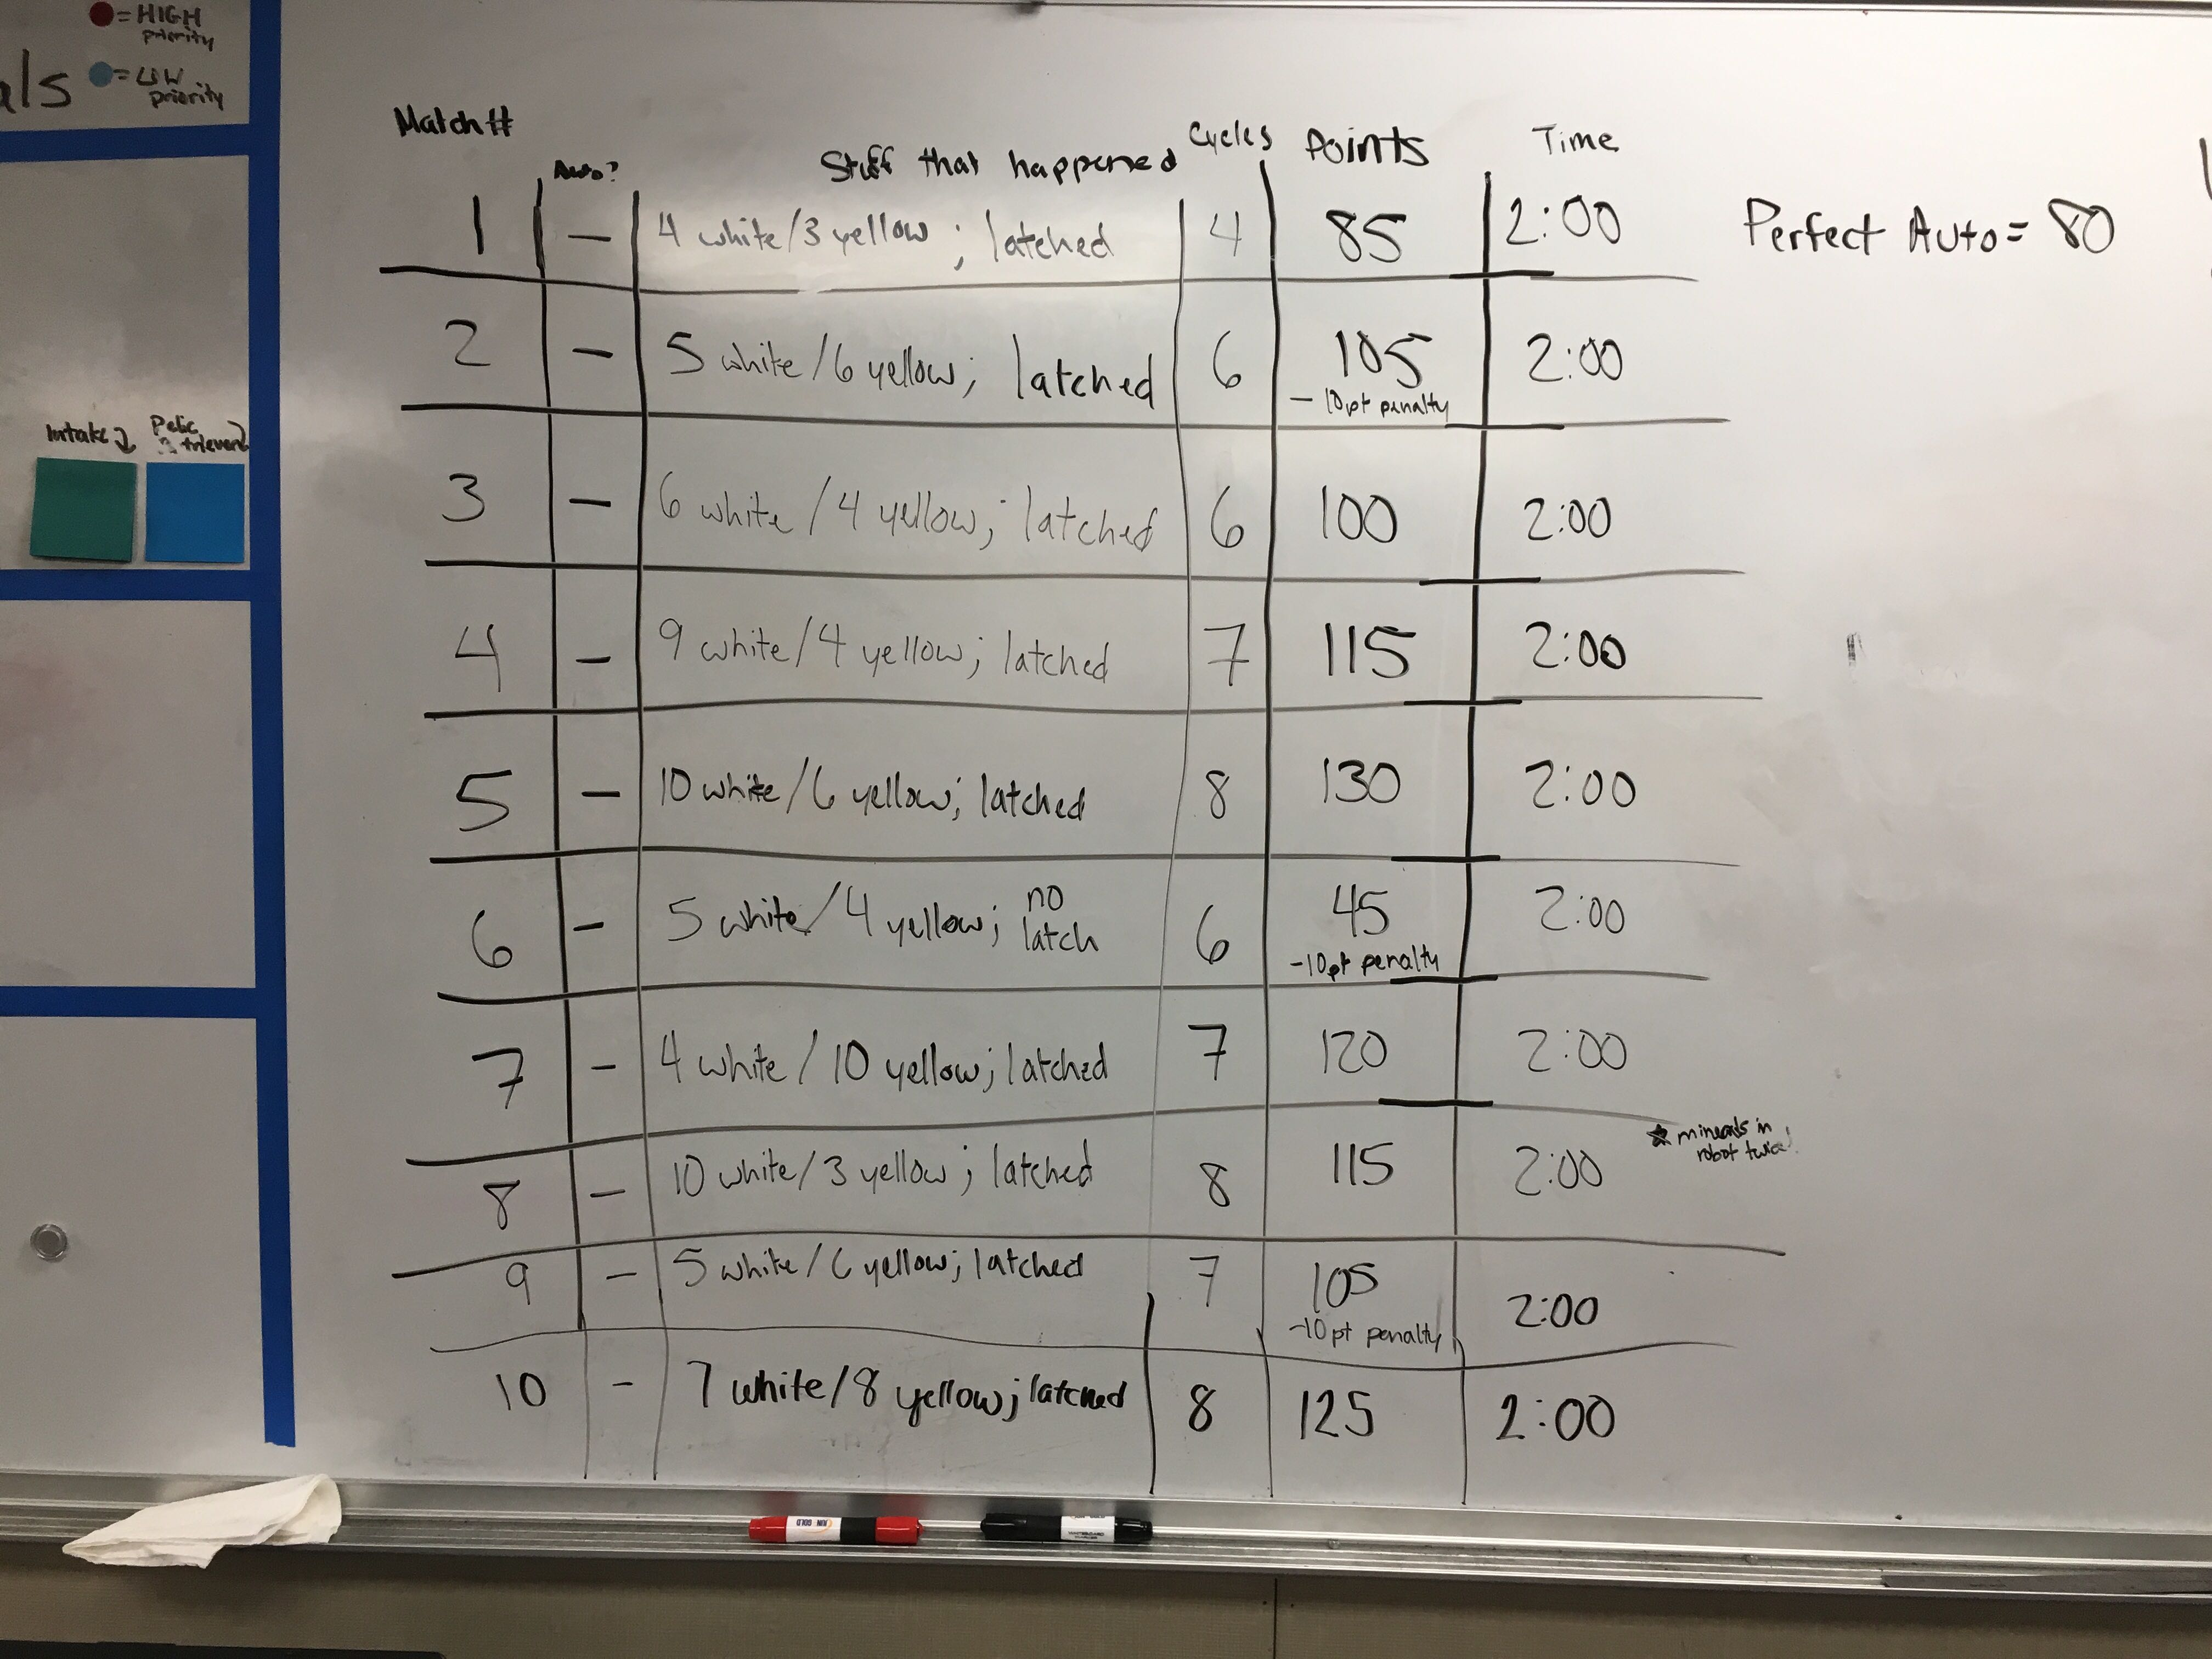
\includegraphics[width=.6 \textwidth]{23_02-04/images/IMG_1512.JPG}
    \caption{Score Keeping Chart}
    \label{fig:chart}
\end{figure}
\end{document}